\documentclass[UKenglish,12pt]{master-style}
\usepackage[utf8]{inputenc}
\usepackage[T1]{fontenc,url}
\usepackage{csquotes}
\usepackage{url}
\urlstyle{sf}
\usepackage{babel,textcomp,csquotes,duomasterforside,varioref,graphicx}
\usepackage[backend=biber,style=numeric-comp]{biblatex}

\usepackage[document]{ragged2e} % If one for some odd reason would like to have a left-aligned text like in Word ;-/
\usepackage{hyperref}           % If one wants hyperlinks in the document...
\hypersetup{
    colorlinks=true,
    citecolor=black,
    filecolor=black,
    linkcolor=black,
    urlcolor=black,
%    linkcolor=blue, please add a % change all to black if the links should not be "visible"
%    filecolor=magenta,      
%    urlcolor=cyan,
    pdftitle={Master Thesis},
    pdfpagemode=FullScreen,
    }


%Add packages as you need them 
\usepackage{blindtext} % Just to create some random text - remove!
\setlength{\parskip}{\baselineskip}

\linespread{1.25} % = 1.5 line spacing in Word


\title{Generative Properties of Image-to-Image Translation Methods}
%\subtitle{Some subtitle?}
\author{Pratima Kumari}

\addbibresource{mybib.bib} 

\begin{document}
\duoforside[%   
    %% ... or your department
    dept={Department of Computer Science},  
    %% ... or your programme
    program={Applied Computer and Information Technology (ACIT)},
    %30 credits = short, 60 credits = long
    short% 
    ]

\frontmatter 

% Preface
\chapter*{Preface}

I would like to take the opportunity here to thank the people that made my master thesis "Generative Properties of Image-to-Image Translation Methods” possible. It is written as part of the Applied Computer and Information Technology master’s program at Oslo Metropolitan University, under Applied Artificial Intelligence specialisation.  

First and foremost,I would like to thank my supervisor, Hugo Lewi Hammer, his expertise, mentorship, and constructive feedback have been very useful in shaping this thesis and broadening my understanding of the subject matter. I would also like to thank my co-supervisor Michael Riegler of SimulaMet. Finally, I want to express my sincere thanks to my colleagues and friends for their companionship and valuable discussions, which have enhanced my academic experience.

In the era of rapid advancements in artificial intelligence and computer vision, image generation has become more and more possible with the introduction of stronger generative artificial intelligence (AI) models. The ability to translate images between different domains is very fascinating and essential research area. This idea and ability of generating non-existing images that highly resemble real world images is the motivation for me to persue my thesis around this area.

Pratima Kumari\\
Oslo, May 2024 

% Add Preface to Table of Contents
\addcontentsline{toc}{chapter}{Preface}

% Abstract
\chapter*{Abstract}

Generative Adversarial Networks (GANs) have emerged as a powerful tool in image-to-image translation tasks  while preserving essential characteristics and in learning mappings between two image domains without the need for paired data. This thesis investigates the generative properties of such methods, focusing on their application to gastrointestinal endoscopy images using the Hyper Kvasir dataset \cite{10.1007/978-3-031-45673-2}. The primary aim is to evaluate the performance of GAN-based models, specifically CycleGAN, in generating translations with diverse and realistic properties, such as varying polyp positions, sizes, and shapes .

The thesis begins by outlining the significance of image augmentation in enhancing AI models while minimizing data collection costs. Deep generative learning approaches, particularly GANs, offer promising results for generating synthetic images to enrich datasets. Image-to-Image translation, a subset of computer vision tasks, involves learning mappings between different domains without paired data. Traditional methods relying on paired data has limitations, which motivates the exploration of CycleGAN, and addresses the issue of using unpaired data \cite{10.1007/978-3-031-45673-2}.

This research explore CycleGAN's performance, particularly in accommodating shape changes alongside color and texture alterations. It proposes architectural modifications and loss functions to balance cycle-consistency and the ability to accommodate shape changes effectively. Furthermore, It serves as a foundational exploration into the generative properties in image-to-image translation methods.Overall, this thesis contributes valuable insights into leveraging deep generative learning for analyzing the generative properties of Image-to-Image translation (I2I) methods in the context of gastrointestinal endoscopy imagery with the use of Hyper Kvasir dataset. 


% Add Abstract to Table of Contents
\addcontentsline{toc}{chapter}{Abstract}


%\chapter*{Acknowledgments} \addcontentsline{toc}{chapter}{Acknowledgments}
%I would like to thank ... * insert looong list here *


\tableofcontents
% \listoffigures
% \listoftables

\mainmatter
\chapter{Introduction}

Artificial intelligence, having its roots back to the late 1940s has witnessed a diverse range of applications over the years. In the late 1990s \cite{SHAO2022118221}, the predominant focus of AI projects was on classical or traditional machine learning methods. However, it shifted in the early 2000s with the rise of artificial neural networks, driven by significant advancements in hardware capabilities, an exponential increase in available data, and the emergence of novel algorithms and architectures facilitating the development of larger and deeper neural networks. This transformative development gave the origin of a new category of machine learning known as deep learning .

In recent decades, the utilization of machine learning (ML) applications in the medical domain has seen a remarkable increase, particularly in diagnostic procedures, processing biological data, and supporting medical professionals \cite{Shad_2021}. This integration has led to enhanced efficiency in wait times and accuracy rates for identifying various diseases and disorders. Among many areas within this domain, Computer Vision (CV) stands out , offering various methodologies and algorithms applicable in biomedical imaging tasks. These tasks include identifying important areas in images and helping doctors classify diseases. The information obtained from patient images greatly helps improve healthcare. Recently, Deep Learning (DL) models have become very advanced in these tasks. This improvement is because DL methods are very good at coming up with complex ideas.

However, one key aspect of Deep Learning models, not just in computer vision but across various applications, is the need for large and varied training datasets. This is essential for ensuring the models can make accurate predictions and avoid overfitting, which is a common problem in complex models. Additionally, in supervised machine learning, datasets with significant imbalances among different classes can lead to biased models and reduced performance \cite{RASHIDI20192374289519873088} . This issue is particularly challenging in biomedical imaging due to limited data availability caused by factors like patient privacy concerns, expensive tests, and potential risks from radiation exposure. Moreover, available datasets often have uneven distributions between disease cases and healthy cases, further complicating the training process. 

To address the challenges produced by data scarcity and class imbalances in medical imaging datasets, Data Augmentation (DA) techniques have garnered attention. These approaches aim to artificially expand the size of datasets used for training ML models, particularly DL models employed in computer vision tasks. However, traditional augmentation techniques have shown limitations in significantly boosting model performance, promoting the exploration of more sophisticated methods.\cite{MUMUNI2022100258}.
In recent years, the Generative Adversarial Networks (GANs) family has emerged as a promising models to augment datasets with imbalanced class distributions. These generative models, specifically Generative Adversarial Networks (GANs), have demonstrated usage across various computer vision and imaging tasks \cite{10.1007/978-3-031-45673-2}. Furthermore, using the capabilities of GANs, particularly the cycleGAN model, has enabled a wide range of Image-to-Image (I2I) translation tasks. Examples include day-to-night image translation, style transfer, seasonal image transformation, satellite image enhancement, and medical image synthesis. 

For instance, in day-to-night image translation, cycleGAN can seamlessly transform daytime scenes into nighttime scenes and vice versa, enhancing surveillance footage or simulating nighttime scenarios for autonomous driving systems \cite{satellite_image}. Likewise, style transfer enables the conversion of photographs to mimic the artistic techniques of celebrated painters such as Vincent van Gogh or Pablo Picasso, fostering creativity within the realm of digital art. Moreover, cycleGAN can be employed for seasonal image transformation, converting images captured during one season into those that resemble another \cite{style_transfer}. This capability finds applications in landscape photography and urban planning, where visualizing seasonal variations is essential. In the realm of medical imaging, cycleGAN excels at synthesizing images across different modalities. It can generate MRI images from CT scans, or produce X-ray images from ultrasound scans, aiding in data augmentation for training medical imaging algorithms and improving diagnostic accuracy. In \ref{fig:winter_summer}, we see two examples of results on season transfer, trained on winter and summer photos of Yosemite from Flickr \cite{unpaired} .

\begin{figure}[ht]
    \centering
    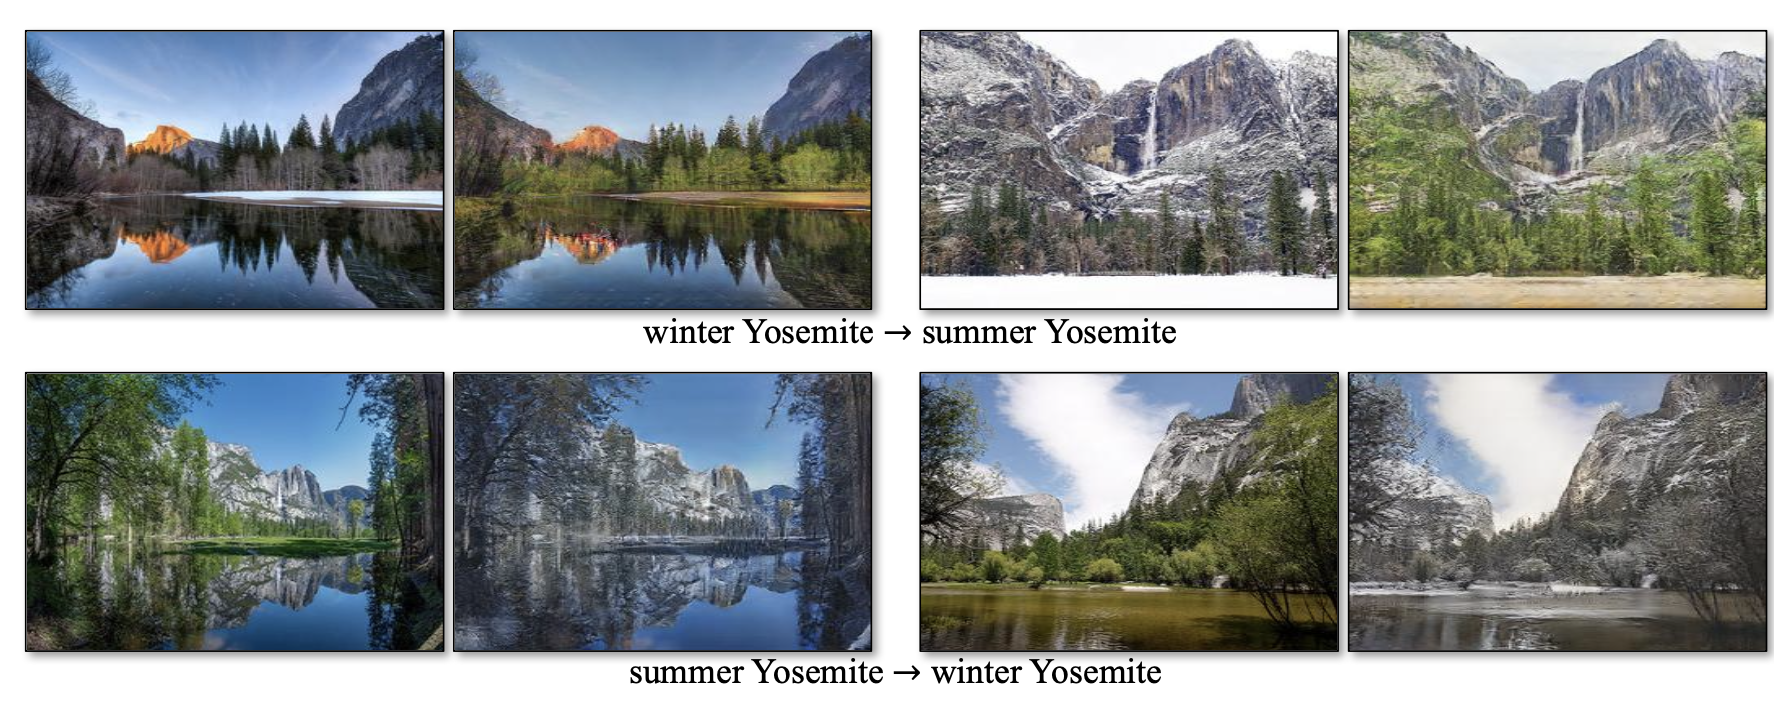
\includegraphics[width=1\textwidth]{Images/winter_summer.png}
    \caption{An example of a season translation from summer - winter}
    \label{fig:winter_summer}
\end{figure}

\section{Motivation}

Medical imaging plays a crucial role in diagnosing and treating various health conditions, providing health experts with valuable insights into the internal structures and abnormalities within the human body \cite{medicalimage}. However, the gathering and labeling of large-scale medical imaging datasets for training machine learning models remain challenging and often limited by factors such as privacy concerns, data scarcity, and the labor-intensive nature of manual labeling. Image-to-Image (I2I) translation methods offer a promising option for addressing these challenges by enabling the generation of synthetic medical images that closely mimic real-world data. By leveraging deep learning techniques, these models can learn to transform images from one domain to another, such as generating pathological variations from healthy images or simulating different disease states within medical imagery \cite{I2I}.

The Hyper Kvasir dataset, with its diverse collection of gastrointestinal endoscopy images, provides a valuable resource for exploring the generative capabilities of I2I translation methods in the context of medical imaging. Specifically, the focus on analyzing the generative properties of these methods with respect to conditions like polyps, which exhibit variability in size, shape, and position, presents an exciting opportunity to evaluate the robustness and realism of synthesized medical imagery. Moreover, by employing the CycleGAN framework, known for its effectiveness in learning image-to-image mappings without paired training data, this research aims to develop a practical solution for generating synthetic medical images directly from the Hyper Kvasir dataset \cite{CycleGAN} . The ability to simulate diverse pathological conditions within endoscopic images not only facilitates the augmentation of existing datasets but also has the potential to enhance the training and evaluation of machine learning algorithms for medical image analysis tasks, such as disease detection and classification.

By addressing these objectives, this master thesis seeks to contribute to the advancement of medical imaging research by providing insights into the capabilities and limitations of I2I translation methods for generating realistic and diverse medical imagery \cite{I2I} . At last, the outcomes of this study have the potential to enhance the efficiency and effectiveness of computer-aided diagnosis systems and pave the way for improved patient care and medical decision-making in clinical settings.

\section{Aim}

The aim of this master thesis is to investigate the generative properties of Image-to-Image (I2I) translation methods using the Hyper Kvasir dataset, specifically focusing on their capability to produce diverse and realistic translations, particularly in the context of medical imagery. The primary focus will be on evaluating the effectiveness of the CycleGAN model in generating synthetic data representative of various medical conditions, such as polyps, by manipulating the size, shape, and position of relevant features within the images.

\section{Research Question and Objectives}

\begin{itemize}
\item \textbf{Objective 1 - Identification of Powerful and Reliable I2I Method. }\\
What constitutes a powerful and reliable method for Image-to-Image translation (I2I) applications, particularly in the context of gastrointestinal endoscopy image enhancement and analysis? How do different I2I methods compare in terms of their effectiveness, efficiency, and robustness in generating accurate translations between different image domains?

\item \textbf{Objective 2 - Analysis of Generative Properties with the Generative Model.}\\
How do the generative properties of the Generative model results when applied to the HyperKvasir dataset for image translation tasks?
To what extent can the Generative model capture and replicate realistic properties, such as variations in polyp positions, sizes, and shapes, in the translated images?

\item \textbf{Objective 3 - Generation of Synthetic Image Data.}\\
Can synthetic image data be effectively generated by introducing blue round shapes at random locations within the original dataset of healthy images from the HyperKvasir dataset? How does the inclusion of synthetic data enhance the diversity and representation of the dataset for training I2I models?

\item \textbf{Objective 4 - Creation of Visual and Qualitative Evaluation Metrics.}\\
What qualitative metrics can be developed to evaluate the performance of I2I models in generating visually realistic translations? How can these metrics effectively capture the accuracy, consistency, and visual quality of the synthetic images produced by the Generative model?

\item \textbf{Objective 5 - Performance Comparison with Ground Truth Data.}\\
How does the performance of the implemented Generative model compare to ground truth data in terms of visual reality, structural accuracy, and pathological relevance? What insights can be gained from the comparison between synthesized images and original data in the context of gastrointestinal endoscopy analysis and diagnosis?

\end{itemize}

\section{Thesis Outline}
\begin{itemize}
\item \textbf{Data Preparation:} Extracting and preprocessing the Hyper Kvasir dataset, ensuring compatibility with the CycleGAN framework.
Implementing methods to introduce synthetic data augmentation, generating blue round shapes at random locations within the images to simulate medical conditions.

\item \textbf{Model Implementation:} Developing and implementing a CycleGAN-based Image-to-Image translation model tailored to the medical imaging domain.
Training the model using the prepared dataset, focusing on optimizing its ability to accurately translate between healthy and polyp image representations.

\item \textbf{Performance Evaluation:}Conducting visual inspections of the generated images to decide how realistic and accurate the translations are, particularly with respect to the variability in size, shape, and position of simulated medical conditions. Assessing the performance of the trained CycleGAN model through quantitative and qualitative measures, including evaluation metrics such as SSIM,PSNR,FID.

\item \textbf{Distribution Analysis:} Analyzing the distribution of generated shapes (e.g., circles representing polyps) within the translated images, evaluating how closely they match with real patterns seen in medical images. Measuring how much the generated images vary, including factors like the size and placement of blue circle imitating polyps, to understand how well the model can generate different and accurate outputs.

\item \textbf{Testing and Validation:} Validating the trained CycleGAN model on a separate testing dataset, evaluating its ability to produce accurate translations on unseen data, highlighting its strengths and limitations in generating realistic medical imagery.

\item \textbf{Documentation and Reporting:} Documenting the methodologies, experimental setup, and results obtained throughout the study in a comprehensive manner. Presenting a detailed analysis of findings, discussing the implications of the results and suggesting potential avenues for future research in the field of medical image synthesis using I2I translation methods.
\end{itemize}


\chapter{Background and Literature Review}

Machine Learning acts as a connection between Statistics and Computer Science, enabling algorithms to learn and improve themselves through initial learning strategies. This approach boosts the efficiency and accuracy of tasks like image translation by using statistical measures and learning structures to process data effectively \cite{app14020496}. The fusion of Machine Learning (ML) with Computer Vision is especially significant. Through the utilization of ML techniques, particularly Image-to-Image translation (I2I) methods utilizing the cycleGAN model, my research aims to explore the generative properties within datasets like the Hyper Kvasir dataset  \cite{I2I}.

Through supervised learning, where labeled data guides models in recognizing patterns and features in images, the cycleGAN model aims to understand the complex relationships between input and output images. This enables the translation of images depicting various gastrointestinal conditions, such as polyps, into visually realistic representations. Moreover, incorporating deep learning principles, characterized by the depth of Artificial Neural Networks (ANNs), highlights the importance of feature extraction in the translation process. This paradigm shift not only transforms image translation tasks but also emphasizes the collaboration between Computer Science and Statistics, as ML algorithms adjust and improve themselves based on learned strategies. Consequently, by delving into machine learning, my thesis seeks to contribute to the evolving fields of Computer Vision and Generative Artificial Intelligence

\section{Convolutional Neural Networks(CNN)}

\vspace{-12pt}Convolutional Neural Networks (CNNs) play a crucial role in driving progress in Image-to-Image translation (I2I) methods, especially in the context of the cycleGAN model applied to the Hyper Kvasir dataset \cite{CNN} . CNNs are extensively used across diverse fields, particularly in Computer Vision (CV), where they act as the cornerstone for analyzing visual data. They facilitate a wide range of tasks, including image classification, segmentation, and object detection. Their hierarchical structure, modeled after the visual cortex in animals, equips them to efficiently leverage spatial relationships within data.

In the goal of analyzing the generative properties of I2I methods, understanding the complexities of CNNs becomes essential. The multilayered architecture of CNNs facilitates hierarchical feature extraction, where successive layers learn and extract more complex features from input images \cite{deep_CNN}. In tasks like image classification, CNNs excel at connecting images with their respective categories by identifying abstract feature representations. In the context of my thesis, the capability of CNNs to autonomously learn distinctive features is crucial for generating lifelike translations of gastrointestinal conditions, like polyps, from the Hyper Kvasir dataset.

The structure of CNNs, organized into convolutional layers, non-linear processing units, and subsampling layers, closely aligns with the iterative process of feature extraction inherent in Image-to-Image (I2I) methods.\cite{CNN} . Through a thorough examination of the architecture and operation of CNNs, my research aims to gain insights that inform the development and optimization of image processing algorithms within the cycleGAN framework. This will ultimately contributes to the progression of medical imaging technology and AI-driven clinical decision support systems by improving the realism and accuracy of translated images. Consequently, this advancement facilitates enhanced diagnostic capabilities in gastroenterology.

\section{Generative Adversarial Networks (GANs)}

\subsection{GAN Network Architectures}

While discriminative models is able to distinguish between different types of data instances (labeled samples), generative models are proficient at creating new data instances (sampling) \cite{medigan}. Unlike modeling decision boundaries within a data space, generative models focus on modeling the distribution of data within that space. Deep generative models typically consist of neural networks with multiple hidden layers, explicitly or implicitly estimating a probability density function (PDF) based on a set of real data samples. By approximating the PDF from observed data points (i.e., learning the distribution of real data), these models can generate new data points by sampling from that distribution. In domains such as computer vision and medical imaging, synthetic images are generated by sampling such unobserved points from high-dimensional imaging data distributions. Various deep generative models, including Variational Autoencoders, Normalizing Flows, Diffusion Models, and Generative Adversarial Networks (GANs), are employed for synthesizing images in these fields. Among these, the GAN framework has achieved widespread adoption in medical imaging applications. Therefore, our focus in this work is primarily on GANs, while acknowledging the potential contributions of other types of generative models.

\begin{figure}[ht]
    \centering
    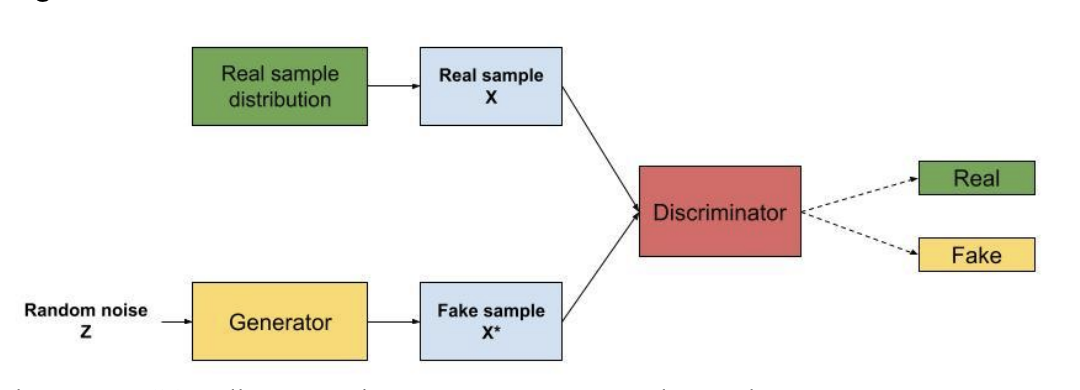
\includegraphics[width=1\textwidth]{Images/GAN_architecture}
    \caption{GAN diagram. The generator uses a random noise vector Z, to generate a fake sample X* which is passed to the discriminator together with a real sample X and the discriminator classifies the fake sample X* real or fake.}
    \label{fig:gan_framework}
\end{figure}

\begin{figure}[ht]
    \centering
    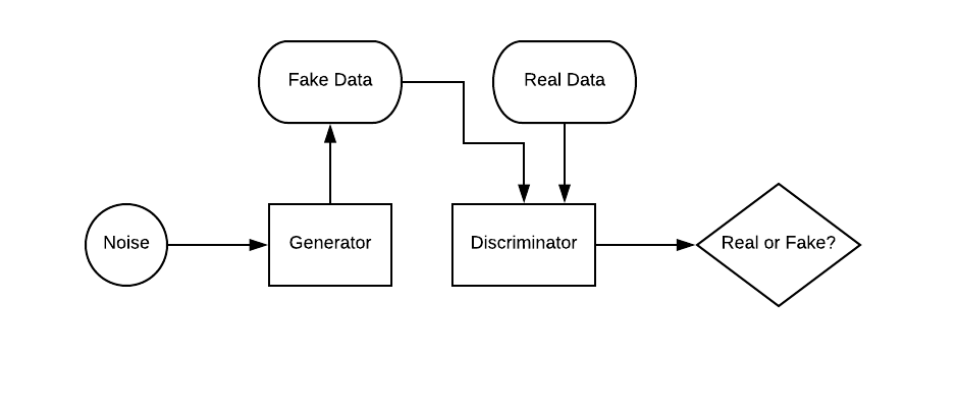
\includegraphics[width=1\textwidth]{Images/GAN.png}
    \caption{Illustration of Generative Adversarial Network}
    \label{fig:GAN}
\end{figure}

In this visual example \ref{fig:gan_framework} and \ref{fig:GAN} \cite{medigan}, the generator network receives random noise vectors, which it learns to map to region-of-interest patches of full-field digital mammograms \cite{GAN} . During training, the adversarial loss is not only backpropagated to the discriminator as LD , but also to the generator as LG. The training of GANs comprises two neural networks, the generator network (G) and the discriminator network (D).

It all began with the introduction of the deep convolutional GAN (DCGAN) architecture, which revolutionized the landscape by providing a foundational framework for both the discriminator (D) and generator (G). Building upon this foundation, furture advancements have been made, including the utilization of more complex architectures such as ResNet-based structures. One notable example of such advancement is the Progressive Growing GAN (PGGAN), which innovatively expands the generator and discriminator networks during training, enabling the synthesis of high-resolution images with remarkable fidelity and detail \cite{medigan}.

In addition to architectural advancements, there has been significant research dedicated to conditioning the output of GANs based on various factors, whether discrete or continuous. Conditional GANs (cGANs), for instance, achieve this by incorporating additional label information into both the discriminator and generator networks\cite{GAN} .
Paired translation approaches, exemplified by pix2pix, employ techniques such as the L1 reconstruction loss alongside the adversarial loss to ensure faithful translation between domains. Conversely, unpaired translation methods, such as cycleGAN, introduce cycle-consistency by enforcing an L1 reconstruction loss between source and target images, ensuring coherence and fidelity during translation \cite{parmar2024onestep}. Beyond these established methodologies, there are ongoing efforts to innovate and push the boundaries of generative modeling. One such innovation is SinGAN, which defies convention by learning to generate multiple synthetic images from just a single training image\cite{syngan}.

\subsection{GANs Training}

Understanding the dynamics of GAN training is very important, as GANs serve as an important component in our image-to-image translation methodology. The Generator initiates the process by taking a vector of random noise sampled from predefined distributions, such as normal or uniform distributions termed as the latent vector. This latent vector serves as the input for the Generator, which then produces synthetic samples  with the objective of mimicking the distribution of real data \cite{8784681} . Conversely, the Discriminator is tasked with assessing the authenticity of the samples it receives, distinguishing between real samples and generated samples. To achieve this, the Discriminator aims to output a value close to 1 when presented with real data, indicating high confidence in its authenticity. Conversely, when presented with generated samples, the Discriminator aims to output a value close to 0, signaling skepticism towards their authenticity.

\begin{figure}[htbp]
    \centering
    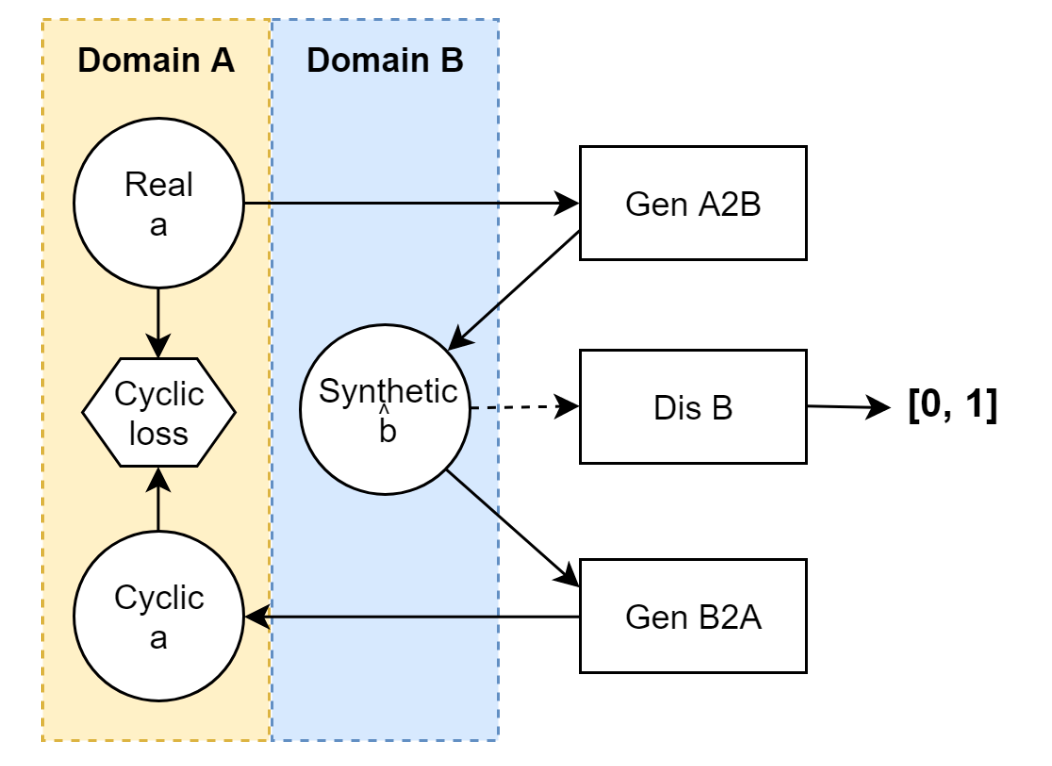
\includegraphics[width=1\textwidth]{Images/Gen_Training.png}
    \caption{Generator training for generator A2B, ’Gen A2B’}
    \label{fig:Gen_Training}
\end{figure}

\begin{figure}[htbp]
    \centering
    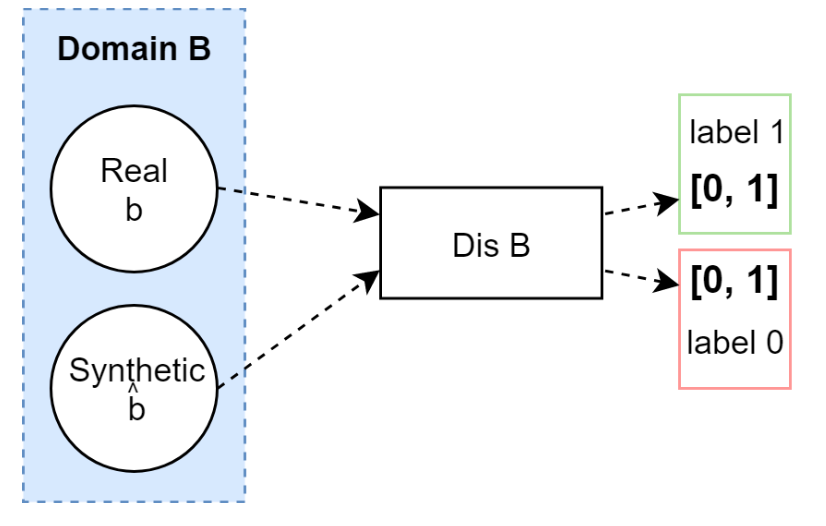
\includegraphics[width=1\textwidth]{Images/Disc_Training.png}
    \caption{Discriminator training for discriminator in domain B, ’Dis B’}
    \label{fig:Disc_Training}
\end{figure}

Figure \ref{fig:Gen_Training} shows Generator training for generator A2B, ’Gen A2B’. Real images in domain A, ’Real a’, flow according to the diagram. The generator weight up- date depends on the cyclic loss and the output from discriminator in domain B, ’Dis B’. The same flow, in the opposite direction, goes for real images from domain B. Both generators are trained on the cyclic losses calculated from both directions. Figure \ref{fig:Disc_Training} shows Discriminator training for discriminator in domain B, ’Dis B’. Discriminator weights are updated depending on the output from real and synthetic images. Real images have ones as labels, synthetic images have zeros. The discriminator in domain A is trained in the same manner, on real and synthetic images in domain A.

The training process of GANs is governed by a cost function, commonly referred to as the Minimax loss, which captures the competitive nature of the Generator-Discriminator interaction. This cost function drives both models towards continuous improvement and adaptation. With each training iteration, gradient steps are taken using backpropagation to minimize the cost function of each network, thereby optimizing their internal parameters \cite{electronics10212689}. Specifically, the Generator is trained to minimize the Jensen–Shannon divergence, measuring the discrepancy between the probability distribution of the generated samples (G(z)) and the expected probability distribution of real data (pdata). This iterative training process continues until convergence, ideally when the Generator generates synthetic data that is indistinguishable from real data, as perceived by the Discriminator.

\subsection{GANs Shortcomings}

Training Generative Adversarial Networks (GANs) presents a complex challenge due to the delicate balance required between the Generator and the Discriminator. 
\begin{enumerate}
    
\item \textbf{{Mode Collapse:}} One common issue encountered in GAN training is Mode Collapse, wherein the Generator is unable to capture the full diversity of the target distribution, resulting in the synthesis of only a limited subset of data. Mode collapse is a prevalent phenomenon observed during the training of Generative Adversarial Networks (GANs), characterized by the Generator's inability to represent the entirety of the target distribution accurately. Instead of generating diverse samples that encompass the full spectrum of possible data, the Generator tends to produce only a limited subset of data, often repeating similar patterns or outputs. This restricted diversity in generated samples fails to capture the richness and complexity of the original distribution, ultimately leading to a loss of variation and fidelity in the synthesized data. Mode collapse poses a significant challenge in GAN training, hindering the network's ability to produce realistic and diverse outputs across different regions of the data space \cite{Kundu_2019_ICCV} .

\item \textbf{{Vanishing Gradient:}} Another challenge in GAN training is the occurrence of Vanishing Gradient, which arises when either the Discriminator or the Generator attains disproportionate power, disrupting the training process \cite{Kundu_2019_ICCV} . This imbalance can prevent the effective propagation of gradients necessary for learning and improvement. When the Discriminator becomes too proficient at distinguishing between real and generated samples, its loss approaches zero, resulting in stagnant gradient feedback to the Generator. As a consequence, the Generator fails to receive meaningful gradients necessary for improving its performance, leading to a stalemate in training. Vanishing gradient poses a significant obstacle in GAN training, requiring careful consideration and mitigation strategies to ensure effective gradient flow and convergence of the network \cite{Kundu_2019_ICCV} .
\end{enumerate}
\section{CycleGAN}

CycleGAN stands out as a versatile tool for transforming images between different domains, even when those images aren't directly paired. Unlike other methods like pix2pix, which rely on paired datasets for training, CycleGAN can work with two separate sets of images without needing them to be explicitly matched. For example, it could take a collection of Monet paintings and a set of landscape photographs and learn to convert images between the two styles. This flexibility extends to medical imaging, where CycleGAN can be used to translate between healthy medical images to unhealthy cancer images, even when they aren't perfectly paired or from the same patients \cite{unpaired_horse2zebra_cyclgan} .

The procedure of cycleGAN is illustrated in Figure \ref{fig:cyclegan}, where G is a generator that translates images
from domain X to domain Y, F is a generator that translates images from domain Y to domain X, DY is a discriminator for both fake and real images in domain Y, and DX is a discriminator for both real and fake images in domain X. The model contains two mappings: G: X → Y and F: Y → X, and two adversarial discriminators DY and DX \cite{unpaired_horse2zebra_cyclgan}. One key feature of CycleGAN is its ability to perform bidirectional translation. This means it learns to translate images from one domain to another (like from paintings to photos) and vice versa, ensuring that the translated images maintain fidelity to the original data. It does this by employing a cycle consistency loss, which ensures that when an image is translated and then translated back, it closely resembles the original image. This consistency helps maintain the integrity of the translation process \cite{unpaired_horse2zebra_cyclgan} .

\begin{figure}[htbp]
    \centering
    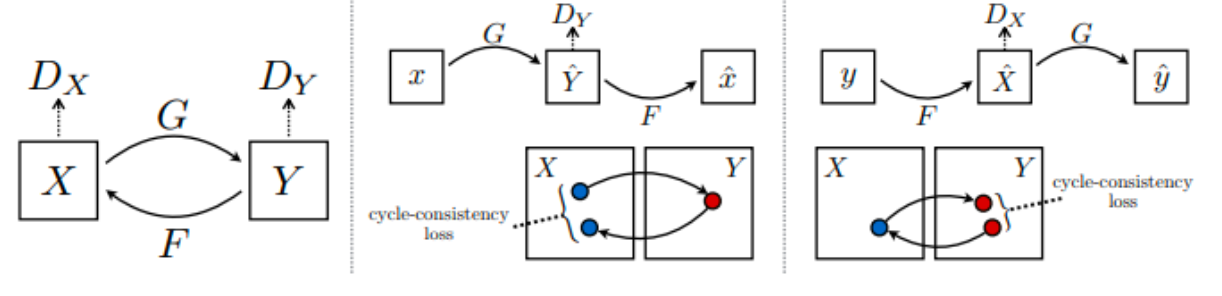
\includegraphics[width=1\textwidth]{Images/cyclegan.png}
    \caption{CycleGAN training procedure}
    \label{fig:cyclegan}
\end{figure}

CycleGAN also uses adversarial loss, employing a technique called Least-Squares GAN (LSGAN). This involves training two discriminators to distinguish between real and generated images, while simultaneously training the generators to produce realistic images that fool the discriminators \cite{unpaired_horse2zebra_cyclgan} . Additionally, an identity mapping loss is incorporated to ensure that real samples from the target domain yield outputs that closely match the input, preserving the authenticity of the original data.
In terms of architecture, CycleGAN typically uses a ResNet-based generator and a PatchGAN discriminator. However, for our project, we've opted for a U-Net-based generator architecture, which offers benefits in capturing finer details and preserving image quality. We've also experimented with different sizes for the PatchGAN discriminator's receptive field to optimize the model's performance

\section{Image-to-Image Translation: Background}

Image-to-image (I2I) models find widespread application across various real-world domains, including industrial, remote sensing, and medical scenarios.  In industrial settings, I2I models serve diverse purposes, including clothes collocating and defect generation. For instance, \cite{application}  introduce a cGAN-based framework designed to collocate clothes by leveraging attributes and categories supervision, resulting in enhanced visual quality through multitask discriminators. Moreover, addressing challenges related to low visibility scenarios, \cite{application}propose a method to translate thermal infrared (IR) images into RGB images. By employing a two-step process involving a Texture-Net architecture and an image colorization network, they enhance textures and details, thereby improving scene perception.

When it comes to defect generation, \cite{application} focus on boundary defects, employing an encoder-decoder network to create a detection hyper-surface in the latent space. This allows for the generation of defects with varying strengths, mimicking different stages of production lines. Additionally, Defect-GAN introduces a method to control both the location and type of defects using SPADE normalization, resulting in the generation of realistic defect samples. Building upon StarGANv2, extend their model to separate background and foreground elements while generating multiple defects, thereby capturing both style and content information.

In case of Remote Sensing Scenarios, \cite{application} propose a method to preserve spectral information and generate unobserved spectral bands from satellite imagery. By considering a shared spectral reconstruction loss, this approach ensures the fidelity of spectral data across multiple satellites. Other techniques combine generation and segmentation methods to synthesize high-quality digital maps or devise strategies for reducing content loss during translation. In medical domains, I2I models find applications in computed tomography (CT), magnetic resonance imaging (MRI), x-ray, and ultrasound. These applications include denoising, segmentation, and cross-modality translation, contributing to advancements in medical image analysis and diagnosis. Supervised approaches often demonstrate superior performance compared to unsupervised ones. To address the challenge of limited paired data,\cite{application} propose generation methods based on radiometry for fabric smoothness assessment, effectively creating a paired dataset for fabric analysis.

\section{Image-to-Image Translation: Other methods}

In this section, we are going to explore various methods other than GANs for Image-to-Image Translation methods: 

\subsection{Pix2pix}

The pix2pix model represents a significant advancement in conditional Generative Adversarial Networks (GANs), specifically tailored for paired image-to-image translation tasks. Unlike traditional GANs, pix2pix incorporates a generator (G) and a discriminator (D), engaging in a zero-sum game to achieve image translation proficiency. The model operates on a dataset comprising pairs of images {xi, yi} where xi belongs to domain X and yi belongs to domain Y \cite{pix2pix} . Each pair exhibits pixel-wise alignment, ensuring correspondence between images from different domains. This alignment enables pix2pix to learn a mapping function G : X → Y, aiming to generate output images G(xi) closely resembling the corresponding real images yi.

In the context of medical imaging, pix2pix holds significant promise for cross-modality image synthesis tasks, such as generating computed tomography (CT) images from magnetic resonance (MR) images and vice versa. By leveraging paired datasets comprising voxel-wise aligned MR and CT scans, pix2pix can effectively learn the complex mappings between different imaging modalities, facilitating the synthesis of clinically relevant medical images \cite{pix2pix} .

\subsection{Diffusion Model}

Diffusion Models (DMs) have emerged as a potent technique in the area of density estimation and sample quality enhancement, showcasing impressive performance across various domains such as images, video, audio, and biomedical data \cite{DiffI2I}. Unlike other generative models like GANs, DMs utilize parameterized Markov chains to optimize the lower variational bound on the likelihood function, enabling them to generate highly precise outputs. Given their recent success in diverse domains, incorporating DMs into Image-to-Image (I2I) models offers a promising avenue to advance the capabilities of I2I tasks significantly.

In recent years, DMs have garnered considerable attention in I2I applications including super-resolution, inpainting, semantic segmentation, and depth estimation. For instance, DM-based approaches like SR3 and SRDiff have demonstrated superior performance in image super-resolution compared to traditional GAN-based methods. Similarly, advancements such as Palette and LDM have applied DMs for image restoration and latent space enhancement in I2I tasks, respectively. Despite these achievements, existing DM frameworks often diffuse over entire images or feature maps, which may not fully align with the constraints of certain I2I tasks, leading to inefficiencies and instability \cite{DiffI2I}.

The preliminary understanding of diffusion models (DMs) entails two fundamental processes: the forward diffusion process and the reverse inference process. During the training phase, DM methods establish a diffusion process using a fixed Markov chain to transform an input image into Gaussian noise through a series of iterations \cite{DiffI2I}. Subsequently, in the inference stage, DM methods sample a Gaussian random noise map and iteratively denoise it to converge on a high-quality output.

\subsection{StarGAN v2}

StarGAN v2 introduces a versatile approach to multi-domain image-to-image translation, enabling the seamless conversion of images across various domains and modalities. Unlike traditional models that require separate generators for each translation direction, such as pix2pix and CycleGAN, starGAN v2 learns multi-modal mappings between domains, offering scalability and efficiency in handling diverse image translation tasks. This model can be trained with sets of medical images from different imaging modalities, such as MR sequences and CT scans. For instance, a single starGAN v2 model could be trained with sets of images representing diverse modalities. Consequently, this trained model can facilitate translations between any combination of these modalities \cite{Chakraborty_2024} .

\subsection{DRIT++}

DRIT++ stands as a recent advancement in the realm of Generative Adversarial Networks (GANs), boasting a higher level of complexity aimed at achieving more diverse output from a single input in the context of unsupervised Image-to-Image (I2I) translation through disentangled representations \cite{comparative_study}. This innovative approach of DRIT++ revolves around the notion of encoding input images into two distinct latent spaces: a domain-invariant content representation and a domain-specific attribute representation. Essentially, the domain-invariant content representation encapsulates the shared information between the two domains, while the domain-specific attribute representation delineates the characteristic features unique to each domain. Leveraging these disentangled representations, DRIT++ synthesizes output images by blending the encoded content and attributes, thereby offering the flexibility for feature-wise transformations that enable greater shape variation.

\subsection{CoMIR}

CoMIR introduces a novel technique for learning representations that exhibit rotation-equivariance in image data, accomplished through an objective function grounded in noise-contrastive estimation (InfoNCE)\cite{comparative_study}. This approach aims to create representations that maintain rotational consistency, typically retaining the same dimensions as the input images. The central component of CoMIR is the InfoNCE loss function, which computes the ratio between joint probabilities and the product of individual probabilities for pairs of images in the dataset. To approximate this ratio, CoMIR employs the exponential function with a critic function and a scaling parameter. The critic function ensures positive symmetry, achieving its maximum when the input values are identical.

\section{Image-to-Image Translation: Network architectures} 

In this section, we explore the details of network architectures in the area of generative modeling, exploring their design principles, functionalities, and applications in the context of image-to-image translation.

\subsection{U-Net}

The initial implementation of pix2pix utilized a U-Net-based generator, a convolutional neural network architecture renowned for its effectiveness in image-to-image translation tasks. U-Net, originally developed for biomedical image segmentation, integrates skip-connections to facilitate information flow between different layers of the network. These skip-connections, which concatenate the output feature maps from earlier layers with the input feature maps of later layers, play a crucial role in preserving spatial information throughout the network \cite{ZUNAIR2021104699} .

The architecture of U-Net is characterized by its distinctive U-shaped design, consisting of a contracting path on the left side and an expansive path on the right side \cite{ZUNAIR2021104699} . The skip connections in U-Net serve as bridges between the contracting and expansive paths, facilitating the fusion of low-level and high-level features extracted from different layers of the network. This fusion process enables the generator to reconstruct detailed and semantically meaningful output images from the input data. 

\subsection{ResNet}

In the original CycleGAN setup, two generators based on ResNet are utilized. However, for this thesis project, we opted for U-Net-based generators for CycleGAN. Meanwhile, the original pix2pixHD model features a ResNet-based global generator, accompanied by ResNet-blocks for the local generator. Similarly, starGAN v2 employs ResNet-based architectures, incorporating pre-activation residual units, for its generator, discriminator, and style encoder \cite{ResNet} .

The introduction of ResNets addressed critical challenges associated with deep neural networks, notably the issues of vanishing and exploding gradients. Historically, these problems were mitigated through techniques like normalized initialization and intermediate normalization layers, which facilitated the convergence of deeper networks. However, the emergence of deep networks led to a new obstacle known as the degradation problem. Despite their increased depth, deeper networks exhibited a peculiar phenomenon where accuracy plateaued and subsequently declined. Remarkably, this degradation was not attributable to overfitting; deeper networks exhibited higher training and test errors compared to their shallower counterparts \cite{ResNet}.

\subsection{PatchGAN}

The PatchGAN discriminator architecture, as seen in pix2pix, CycleGAN, pix2pixHD, and the modified pix2pix models (pix2pixM→C and pix2pixC→M), is a pivotal component utilized across various image-to-image translation tasks \cite{patch_gan}. This architecture, denoted by N × N PatchGAN, employs a convolutional neural network (CNN) trained to distinguish overlapping image patches of size N × N as either real or fake.

Compared to alternative architectures such as full-image discriminators, the PatchGAN discriminator offers several advantages. Primarily, it exhibits a more parsimonious parameterization, resulting in a more computationally efficient and tractable model. By focusing on local image patches rather than analyzing the entire image at once, the PatchGAN discriminator achieves a balance between computational complexity and discriminative capacity, making it well-suited for various image translation tasks \cite{patch_gan}.

\section{Image-to-Image Translation methods: Limitations and solutions}

I2I models, while promising for various applications, encounter several challenges that necessitate careful consideration and innovative solutions to enhance their efficacy across different domains. Let's delve deeper into each of these limitations and proposed remedies:

\begin{enumerate}
\item Mode Collapse and Training Instability

Adversarial training, a cornerstone of I2I models \cite{application}, is susceptible to mode collapse and training instability due to the intricate nature of the optimization landscape. This instability can hinder convergence and limit the diversity of generated outputs. To mitigate these issues, researchers have explored alternative loss functions such as LSGAN and Wasserstain distance metric. Additionally, regularization techniques and decoupled loss functions have been introduced to stabilize training and prevent mode collapse. By addressing these challenges, models can achieve more robust and diverse image translations.

\item Imbalanced or Limited Data

The imbalance or scarcity of data poses significant challenges for I2I models, affecting the quality of learned representations. In real-world scenarios \cite{application}, datasets often exhibit class-imbalance or may be limited in size, leading to biased translations and suboptimal performance. To overcome these challenges, researchers have proposed various strategies. These include leveraging additional data sources, employing data augmentation techniques such as convex interpolation, and exploring knowledge distillation procedures. By augmenting the training data and incorporating domain knowledge, models can better capture the underlying distribution and generate more accurate translations.

\item Metrics

Assessing the quality of synthesized images remains a challenge due to the limitations of existing metrics. Metrics like FID and LPIPS \cite{application} provide valuable insights but may not fully capture important aspects such as perceptual similarity and domain-specific attributes. To complement quantitative analysis, researchers often resort to qualitative assessments involving human subjects. These studies offer valuable qualitative feedback and help validate the effectiveness of I2I models in capturing desired characteristics.

\item Large Models

Deploying large-scale I2I models on resource-constrained devices presents significant obstacles. These models often require extensive computational resources and memory, making them unsuitable for edge deployment. To address this issue \cite{application}, researchers have explored various techniques such as model compression, weight sharing, and subnetwork utilization. By reducing model complexity and optimizing resource usage, models can be tailored for deployment on low-powered edge devices without compromising performance.

\item Validation

The lack of comprehensive validation studies, particularly in critical domains like medicine and industry, poses a significant hurdle to the widespread adoption of I2I models \cite{application}. Privacy concerns, scarcity of pre-trained architectures, and challenges in reproducing operational settings further exacerbate this issue. Robust validation methodologies tailored to specific application domains are essential to assess the reliability and effectiveness of I2I models accurately. By addressing these validation challenges, researchers can build confidence in the practical applicability of I2I models across diverse domains.

\end{enumerate}

\section{Gastrointestinal abnormality detection}

Gastrointestinal (GI) infections and cancer represent significant health challenges worldwide, often leading to high mortality rates. Notably, the United States reports a high incidence of gastric cancer, with approximately 1.6 million cases of bowel infections and 0.2 million new cases reported annually \cite{Gastrointestinal}. 
Gastroenterologists play a crucial role in examining and interpreting gastrointestinal tract images and videos. Endoscopy, a primary imaging modality, plays a vital role in detecting and diagnosing GI abnormalities, offering both diagnostic and therapeutic capabilities. 

In recent years, deep learning approaches, such as CycleGAN, have emerged as promising tools for medical image analysis. Unlike traditional machine learning methods, deep learning techniques automatically extract relevant features from data, making them well-suited for tasks involving large and complex medical datasets. CycleGAN, specifically, offers a powerful framework for image-to-image translation tasks, enabling the transformation of images from one domain to another. Early diagnosis of GI conditions is essential for effective management and treatment. As the volume of GI-related data continues to increase, the need for efficient AI systems becomes imperative to minimize diagnostic errors and support healthcare professionals. Deep learning methods, including CycleGAN, hold particular promise for medical imaging tasks, offering the potential to enhance diagnostic accuracy and efficiency \cite{CycleGAN} . By leveraging CycleGAN for image-to-image translation in GI abnormality detection, researchers can explore innovative approaches to improving diagnostic capabilities, ultimately leading to better patient outcomes and reduced healthcare burdens.

Previous studies have proposed various techniques for the effective detection and diagnosis of abnormalities in the digestive system, utilizing both real-time image data collected from hospitals and publicly available datasets.  HyperKvasir, an upgraded version of the Kvasir dataset, offers a vast repository of data for researchers studying GI tract diseases \cite{HyperKvasir_Dataset}. Although still relatively underexplored, HyperKvasir has been used in various studies. The demand for digitized medical images has surged in recent years to extract useful features, facilitating better abnormality detection. The integration of EWT with deep learning can enhance disease detection by extracting specific feature patterns from images, thus motivating further research in the domain of alimentary canal disease detection within gastroenterology.

\section{HyperKvasir Dataset}

The Hyperkvasir dataset \cite{HyperKvasir_Dataset} is a collection of medical images and videos,  created to support research in gastroenterological image analysis. It is categorized into four main sections: labeled image data, unlabeled image data, segmented image data, and annotated video data. Each section provides valuable resources for various machine learning and computer vision tasks, particularly in the context of medical imaging and disease diagnosis.

\begin{figure}[ht]
    \centering
    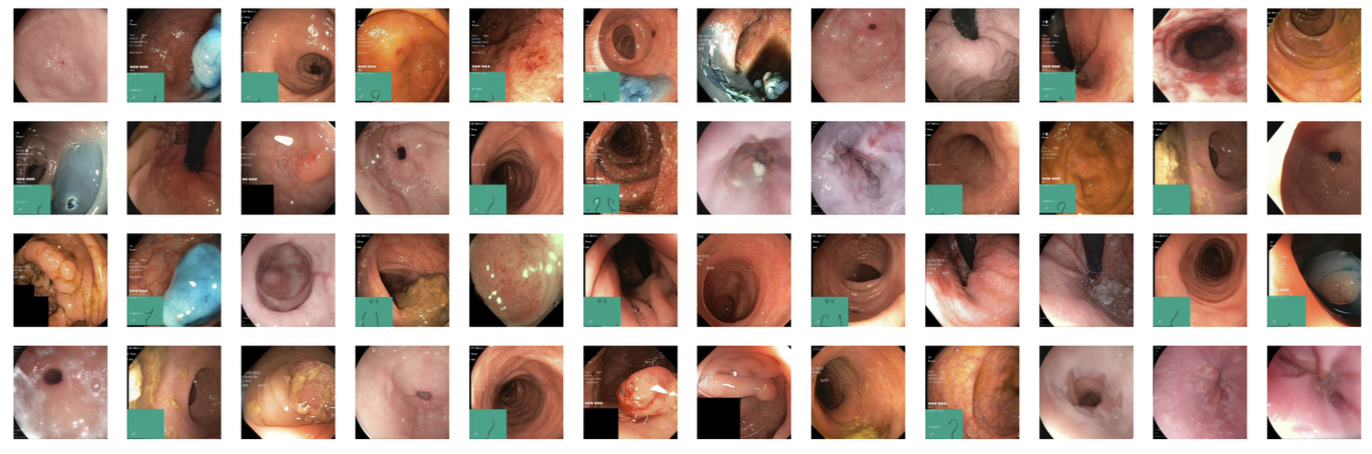
\includegraphics[width=1\textwidth]{Images/hyperKvasir.png}
    \caption{A sample from the HyperKvasir dataset showing images from the upper and lower GI tract.}
    \label{}
\end{figure}

\textbf{Dataset Characteristics:} The Hyperkvasir dataset includes a large collection of labeled images, totaling 10,662 in JPEG format. These images are carefully organized based on the medical findings they depict, covering a wide range of gastroenterological conditions. The class distribution within this section is not uniform, reflecting the natural diversity found in medical datasets, where some conditions are more common than others. The labeled images cover 23 distinct classes of findings, providing a diverse and comprehensive set of cases for analysis and training in medical image analysis tasks \cite{HyperKvasir_Dataset}. In addition to the labeled images, the Hyperkvasir dataset consist of a large repository of unlabeled images, totaling 99,417 in number. A subset of the Hyperkvasir dataset consists of segmented images, which provide valuable insights into specific anatomical structures and pathologies. The dataset also features annotated videos, comprising a total of 373 videos capturing various gastroenterological findings and landmarks. 

\textbf{Significance in Image-to-Image Translation: } The HyperKvasir dataset has been identified as a valuable resource for research in image-to-image translation, as demonstrated in the medigan library paper \cite{medigan}.  The medigan library, a Python library of pretrained generative models, utilizes the HyperKvasir dataset as one of the benchmarks to evaluate the performance of its synthetic data generation capabilities. 

The HyperKvasir dataset, with its diverse and comprehensive collection of gastrointestinal endoscopy images, provides an excellent testbed for evaluating the effectiveness of image-to-image translation techniques in the medical imaging domain. The diverse and high-quality images in the HyperKvasir dataset serve as valuable training data for generative models to learn realistic mappings between different image domains. GANs trained on this dataset can generate synthetic images that closely resemble real endoscopy images, facilitating tasks such as data augmentation and domain adaptation.

By leveraging HyperKvasir dataset for this thesis, the study aims to research the generative properties of CycleGANs in the context of image-to-image translation, with a specific focus on exploring the model's ability to capture domain-specific features, preserve semantic content, and produce visually convincing translations between the horse and zebra domains.

\section{Horse2zebra Dataset}

The Horse2Zebra dataset also serves as a fundamental resource in the area of image-to-image translation, particularly in the context of Generative Adversarial Networks (GANs) and CycleGAN models. This dataset comprises paired images, with one set depicting horses and the other set portraying zebras. Each pair represents semantically similar images but from different domains, facilitating supervised training for models aiming to translate images between these domains \cite{unpaired_horse2zebra_cyclgan}.


\begin{figure}[ht]
    \centering
    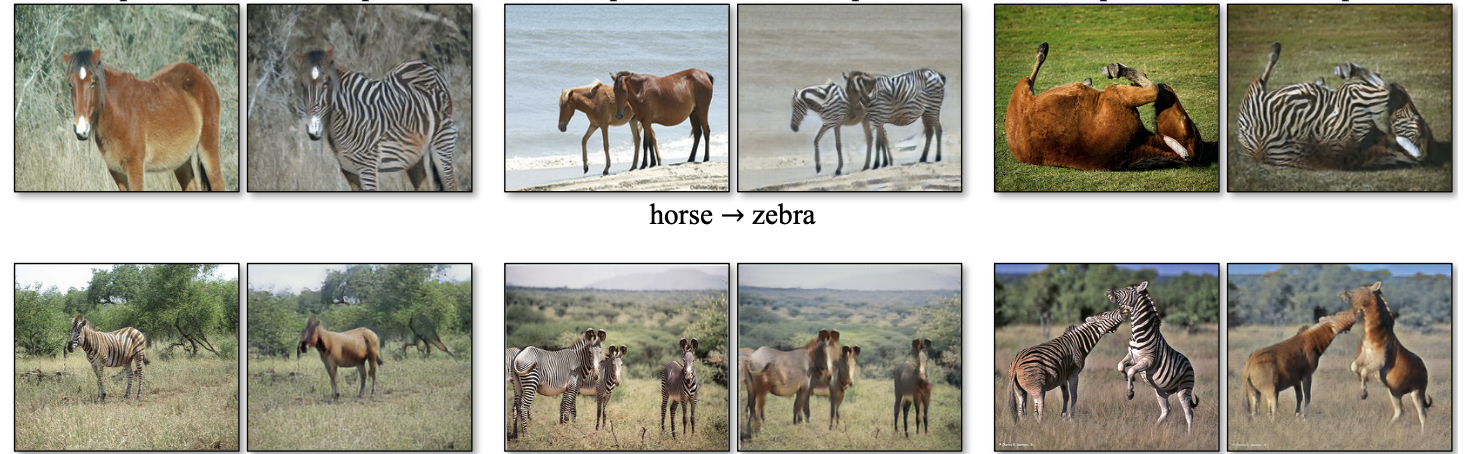
\includegraphics[width=1\textwidth]{Images/horse2zebra.png}
    \caption{A sample from the Horse2Zebra dataset}
    \label{fig:horse2zebra}
\end{figure}

\textbf{Dataset Characteristics:} Each image in the Horse2Zebra dataset , as shown in figure \ref{fig:horse2zebra} has a corresponding image in the other domain, ensuring a clear mapping between the two domains. The dataset shows variability in terms of pose, lighting conditions, background, and other environmental factors, reflecting real-world scenarios and challenges encountered in image translation tasks. Images in the dataset typically maintain a standard resolution and quality, enabling consistent training procedures and model evaluation \cite{unpaired_horse2zebra_cyclgan}.

\textbf{Significance in Image-to-Image Translation: }The Horse2Zebra dataset holds importance in advancing the, specifically CycleGANs. It serves as a benchmark dataset for evaluating the performance of image translation models, allowing researchers to compare the effectiveness of different approaches in achieving realistic translations. The dataset's has complexity, with variations in appearance and environmental conditions, challenges models to learn robust representations and generate realistic translations, contributing to the advancement of state-of-the-art techniques. Models trained on the Horse2Zebra dataset demonstrate the ability to generalize across different datasets and domains, showcasing the adaptability and versatility of CycleGANs in handling diverse image translation tasks. Researchers use the Horse2Zebra dataset for exploring novel architectures, loss functions, and training strategies, aiming to enhance the generative properties and convergence behavior of image translation models \cite{unpaired_horse2zebra_cyclgan}.

\section{Evaluation Metrics}

The evaluation of Image-to-Image (I2I) translation methods is essential for understanding the performance and effectiveness of these models in generating realistic and high-quality images.To quantitatively measure the similarity between the generated images for our datasets and their corresponding truth images, in future we are going to utilize few widely-employed evaluation metrics: .
\begin{itemize}

\item \textbf{Visual Inspection and Human Evaluation}:

Despite the availability of quantitative metrics, visual inspection and human evaluation remain the most important metrics for assessing the quality and reality of generated images. We will evaluate the translated images subjectively, looking at how closely they resemble the originals, how realistic they appear, how coherent they are, and their overall visual appeal. Visual inspection and human evaluation enhance our understanding of the image-to-image translation model,, providing a more comprehensive understanding of the strengths and limitations of the I2I translation model \cite{I2I} .

\item \textbf{FID Score (Fréchet Inception Distance):}

FID score is a widely-used metric that quantifies the similarity between the distribution of real images and generated images. It measures the distance between feature representations extracted from a pre-trained deep convolutional neural network, such as InceptionNet. A lower FID score indicates a higher similarity between the distributions of real and generated images, signifying better image quality and distribution matching \cite{FID} .

\item \textbf{Structural Similarity Index (SSIM}:

The Structural Similarity Index (SSIM) is a metric commonly used to evaluate the similarity between two images. It measures the similarity in structural information, including luminance, contrast, and structure. SSIM values range between -1 and 1, where a value closer to 1 indicates higher similarity between the images \cite{evaluation} .

\item \textbf{Peak Signal-to-Noise Ratio (PSNR)}:
Peak Signal-to-Noise Ratio (PSNR) is a metric used to measure the quality of reconstructed images. It calculates the ratio of the maximum possible power of a signal and the power of corrupting noise that affects the fidelity of its representation. PSNR is expressed in decibels (dB), and higher values signify better image quality\cite{evaluation}  .

\item \textbf{Mean Absolute Error (MAE)}:
Mean Absolute Error (MAE) measures the average absolute differences between corresponding elements of the generated and ground truth images. It provides a simple and intuitive measure of the dissimilarity between the images. Lower MAE values indicate better alignment between the images \cite{evaluation} .

\end{itemize}

\chapter{Methodology}
\section{Experimental Setup}
In this section, we provide an overview of the experimental setup for our proposed method of Image-to-Image translation (I2I) using CycleGAN  \cite{CycleGAN} on Hyper Kvasir dataset \cite{HyperKvasir_Dataset}. Our approach involves a series of steps designed to ensure robust training and accurate translation of images. The experimental setup encompasses software tools, preprocessing of the dataset, and the training procedure for CycleGAN model.

The method developed and implemented in this thesis can be summarized below:

\begin{itemize}

\item \textbf{Step1:} Generating synthetic data by incorporating blue round shapes, simulating polyps, into the original images from the HyperKvasir dataset. These synthetic polyps will vary in size and shape and will be placed at random locations within the images.

\item \textbf{Step2:} Preprocessing of Hyper Kvasir Dataset by resizing images to a uniform dimension, normalize pixel values, and augment the dataset with synthetic data.

\item \textbf{Step3: }Splitting the dataset into training and testing sets, ensuring data integrity and preventing overfitting and to validate model performance.

\item \textbf{Step 4:}Training Procedure to implement the CycleGAN architecture using pyTorch, define hyperparameters, and training the model on the preprocessed dataset.

\item \textbf{Step 5: }Qualitatively assessing the visual quality of generated images and Quantitatively evaluating the model's performance using SSIM, PSNR, and FID score.

\item \textbf{Step 6: }Analyzing the distribution of blue circle region in Synthetic images and translated images.
\end{itemize}

\section{Selection of Model : Diffusion Model or CycleGAN Model}

The selection of the appropriate model architecture for image-to-image translation tasks, such as transforming healthy images to cancer images with polyps, is crucial for achieving the research objectives effectively. In this section, I will provide the reasoning behind choosing CycleGAN over the diffusion model, addressing the specific research questions outlined in the aim of the thesis.

\textbf{Scope and Complexity of the Task:}
The research objective of this thesis involves generating translations between healthy images and cancer images with polyps while preserving realistic properties such as different positions, sizes, and shapes of polyps. This task involves complex transformations in both appearance and semantics.
CycleGAN is well-suited for such complex image-to-image translation tasks, as it is designed to learn mappings between two domains without requiring paired training data. Its ability to capture  complex relationships between the input and output image between domains makes it suitable for handling variations in polyp appearances and positions.
In contrast, while diffusion models have shown impressive performance in generating high-quality images, they are typically better suited for unconditional image generation tasks, where the model learns to generate images from scratch without any input. Applying diffusion models to your specific I2I translation problem may require additional modifications or constraints to ensure the generated cancer images with polyps match the characteristics of the input healthy images, which could be more challenging to implement.

\textbf{Generative Properties and Realism:}
The primary focus of the research is to analyze the generative properties of image-to-image translation methods, particularly in generating translations with different realistic properties.
CycleGAN has demonstrated remarkable capabilities in generating diverse and realistic translations by leveraging cyclic consistency loss. This ensures that the translated images maintain semantic consistency with the input, which is essential for preserving realistic properties such as polyp positions and shapes.

Diffusion models, while capable of generating high-quality images, may not always prioritize the preservation of specific object properties, such as the position, size, and shape of the polyps. Adapting diffusion models to our specific task of translating between healthy and cancer images with varying polyp characteristics may require additional architectural modifications or loss functions, which could increase the complexity of our implementation and analysis.

\textbf{Dataset Compatibility:}
The Hyper Kvasir dataset, chosen for this research, contains a diverse range of gastrointestinal images encompassing various pathologies, including polyps. It is essential to select a model that can effectively leverage the dataset's diversity and complexity.
CycleGAN has been successfully applied to a wide range of image translation tasks across different domains and datasets, including medical imaging datasets. Its flexibility and adaptability make it suitable for accommodating the variations present in the Hyper Kvasir dataset.

\textbf{Training Efficiency and Resource Requirements:}
Considering the constraints of time and computational resources in the research environment, it is crucial to select a model that offers a balance between performance and computational efficiency.
CycleGAN, compared to the diffusion model, typically requires fewer computational resources and training time while still achieving competitive results in image-to-image translation tasks. This makes it a practical choice for conducting experiments and analysis within the scope of the master's thesis.

\textbf{Availability of Existing Implementations}
The CycleGAN model has been widely adopted and studied in the field of I2I translation, with various open-source implementations and pre-trained models available. This has facilitated our implementation and experimentation process, as we leveraged existing code and resources to focus on our specific research objectives.
On the other hand, while diffusion models have gained significant attention in the image generation domain, their application to I2I translation tasks may be less explored, and the availability of ready-to-use implementations may be more limited. Developing a custom diffusion model architecture and training pipeline for our specific problem could require a more substantial investment of time and effort, which may not be feasible within the scope of our master's thesis.

In conclusion, the decision to utilize CycleGAN over the diffusion model for the master's thesis on analyzing the generative properties of image-to-image translation methods is justified based on its suitability for handling the complexities of the task, its proven capabilities in generating realistic translations, compatibility with the chosen dataset, and efficiency in terms of training resources. This choice aligns with the research objectives and facilitates the comprehensive analysis of image translations in the context of gastrointestinal imaging with polyps.

\section{Software Tools and Libraries}

The implementation of the Image-to-Image translation (I2I) experiment, particularly utilizing the CycleGAN model on the Hyper Kvasir dataset, use several software tools and libraries in Python. These tools enable efficient development, training, and evaluation of the models. Below are the important libraries used in this experiment:
\begin{itemize}

\item \textbf{PyTorch: }PyTorch is a popular open-source deep learning framework that provides a flexible and dynamic computational graph. It offers modules and functionalities for building and training neural networks efficiently \cite{PyTorch_horse2zebra}.

\item \textbf{torchvision:} torchvision is a PyTorch library that provides utility functions, datasets, and transforms for working with computer vision tasks. In this experiment, torchvision is utilized for image data processing and manipulation, including transformations and dataset handling \cite{PyTorch_horse2zebra}.

\item \textbf{torch.optim: }The torch.optim module provides optimization algorithms for training neural networks. It includes various optimization methods such as Adam, which is widely used for optimizing model parameters during training.

\item \textbf{torch.utils.data:} This module in PyTorch provides utilities for loading and processing data in parallel, making it easier to work with datasets and data loaders. It allows efficient batching, shuffling, and loading of data samples during training.

\item \textbf{matplotlib: }Matplotlib is a comprehensive library for creating static, animated, and interactive visualizations in Python. It is used in this experiment for generating plots and visualizations, particularly for displaying image samples during training.

\item \textbf{tqdm: }tqdm is a Python library that provides a fast, extensible progress bar for loops and iterables. It offers a convenient way to track the progress of operations, such as training epochs or data loading, with minimal overhead.

\item \textbf{PIL (Python Imaging Library):} PIL is a library for opening, manipulating, and saving many different image file formats. It is used here for loading and processing image data from files.

\item \textbf{glob: }The glob module in Python provides a way to search for files with specific patterns. It is used for retrieving file paths matching certain criteria, such as image files in directories.
\end{itemize}

These tools and libraries  \cite{PyTorch_horse2zebra} collectively enable the implementation of the CycleGAN model for Image-to-Image translation tasks on the Hyper Kvasir dataset. They facilitate data preprocessing, model development, training loop execution, and result visualization, contributing to a streamlined and efficient experimental setup.

\section{Dataset}

For experimentation and validation of the CycleGAN model, we utilized three distinct datasets:
\begin{itemize}

\item \textbf{Horse-to-Zebra Dataset: }To experiment the CycleGAN model implementation, we started with the well-known horse-to-zebra dataset. This allowed us to assess the model's performance on more complex and diverse real-world data \cite{PyTorch_horse2zebra}. 

\item \textbf{Hyper Kvasir Dataset:} Finally, we employed the CycleGAN model on the Hyper Kvasir dataset, comprising gastrointestinal endoscopic images. This dataset presented unique challenges due to its medical context and diverse abnormalities, providing an ideal platform for evaluating the model's effectiveness in medical image translation tasks \cite{pytorch_hyperkvasir}. 

\end{itemize}

\section{Generation of Synthetic Data}

Generating synthetic data is a crucial step in enhancing our dataset for training machine learning models. In our case, we aim to create more examples of gastrointestinal abnormalities, like polyps, to better understand how well our model can translate images. To do this, we developed a process to add synthetic abnormalities to original images from our HyperKvasir dataset. The Synthetic Images are generated by adding synthetic polyps to the Original Images. The synthetic polyps are circular and colored blue to distinguish them from real polyps in the dataset. The size of each synthetic polyp is chosen randomly within a predefined range. This gives a variation in polyp sizes within the generated data. The location of each synthetic polyp on the healthy image is also chosen randomly. This introduces variability in the location and size of blue circle polyps, imitating the variety of actual polyps found in colonoscopies.

Our approach involves adding blue circular shapes randomly onto the images. These shapes simulate the appearance of polyps and help introduce variety into our dataset. Here's how our method works: First, we select an image from our original dataset. Then, we randomly choose a position within the image and a size for the blue circle. Next, we draw the blue circle onto the image at the chosen position. This process is repeated for each image in our dataset. This process produces the set of "Synthetic Images". This is implemented with the use of PIL library in python \cite{PyTorch_horse2zebra}.

\begin{figure}[ht]
    \centering
    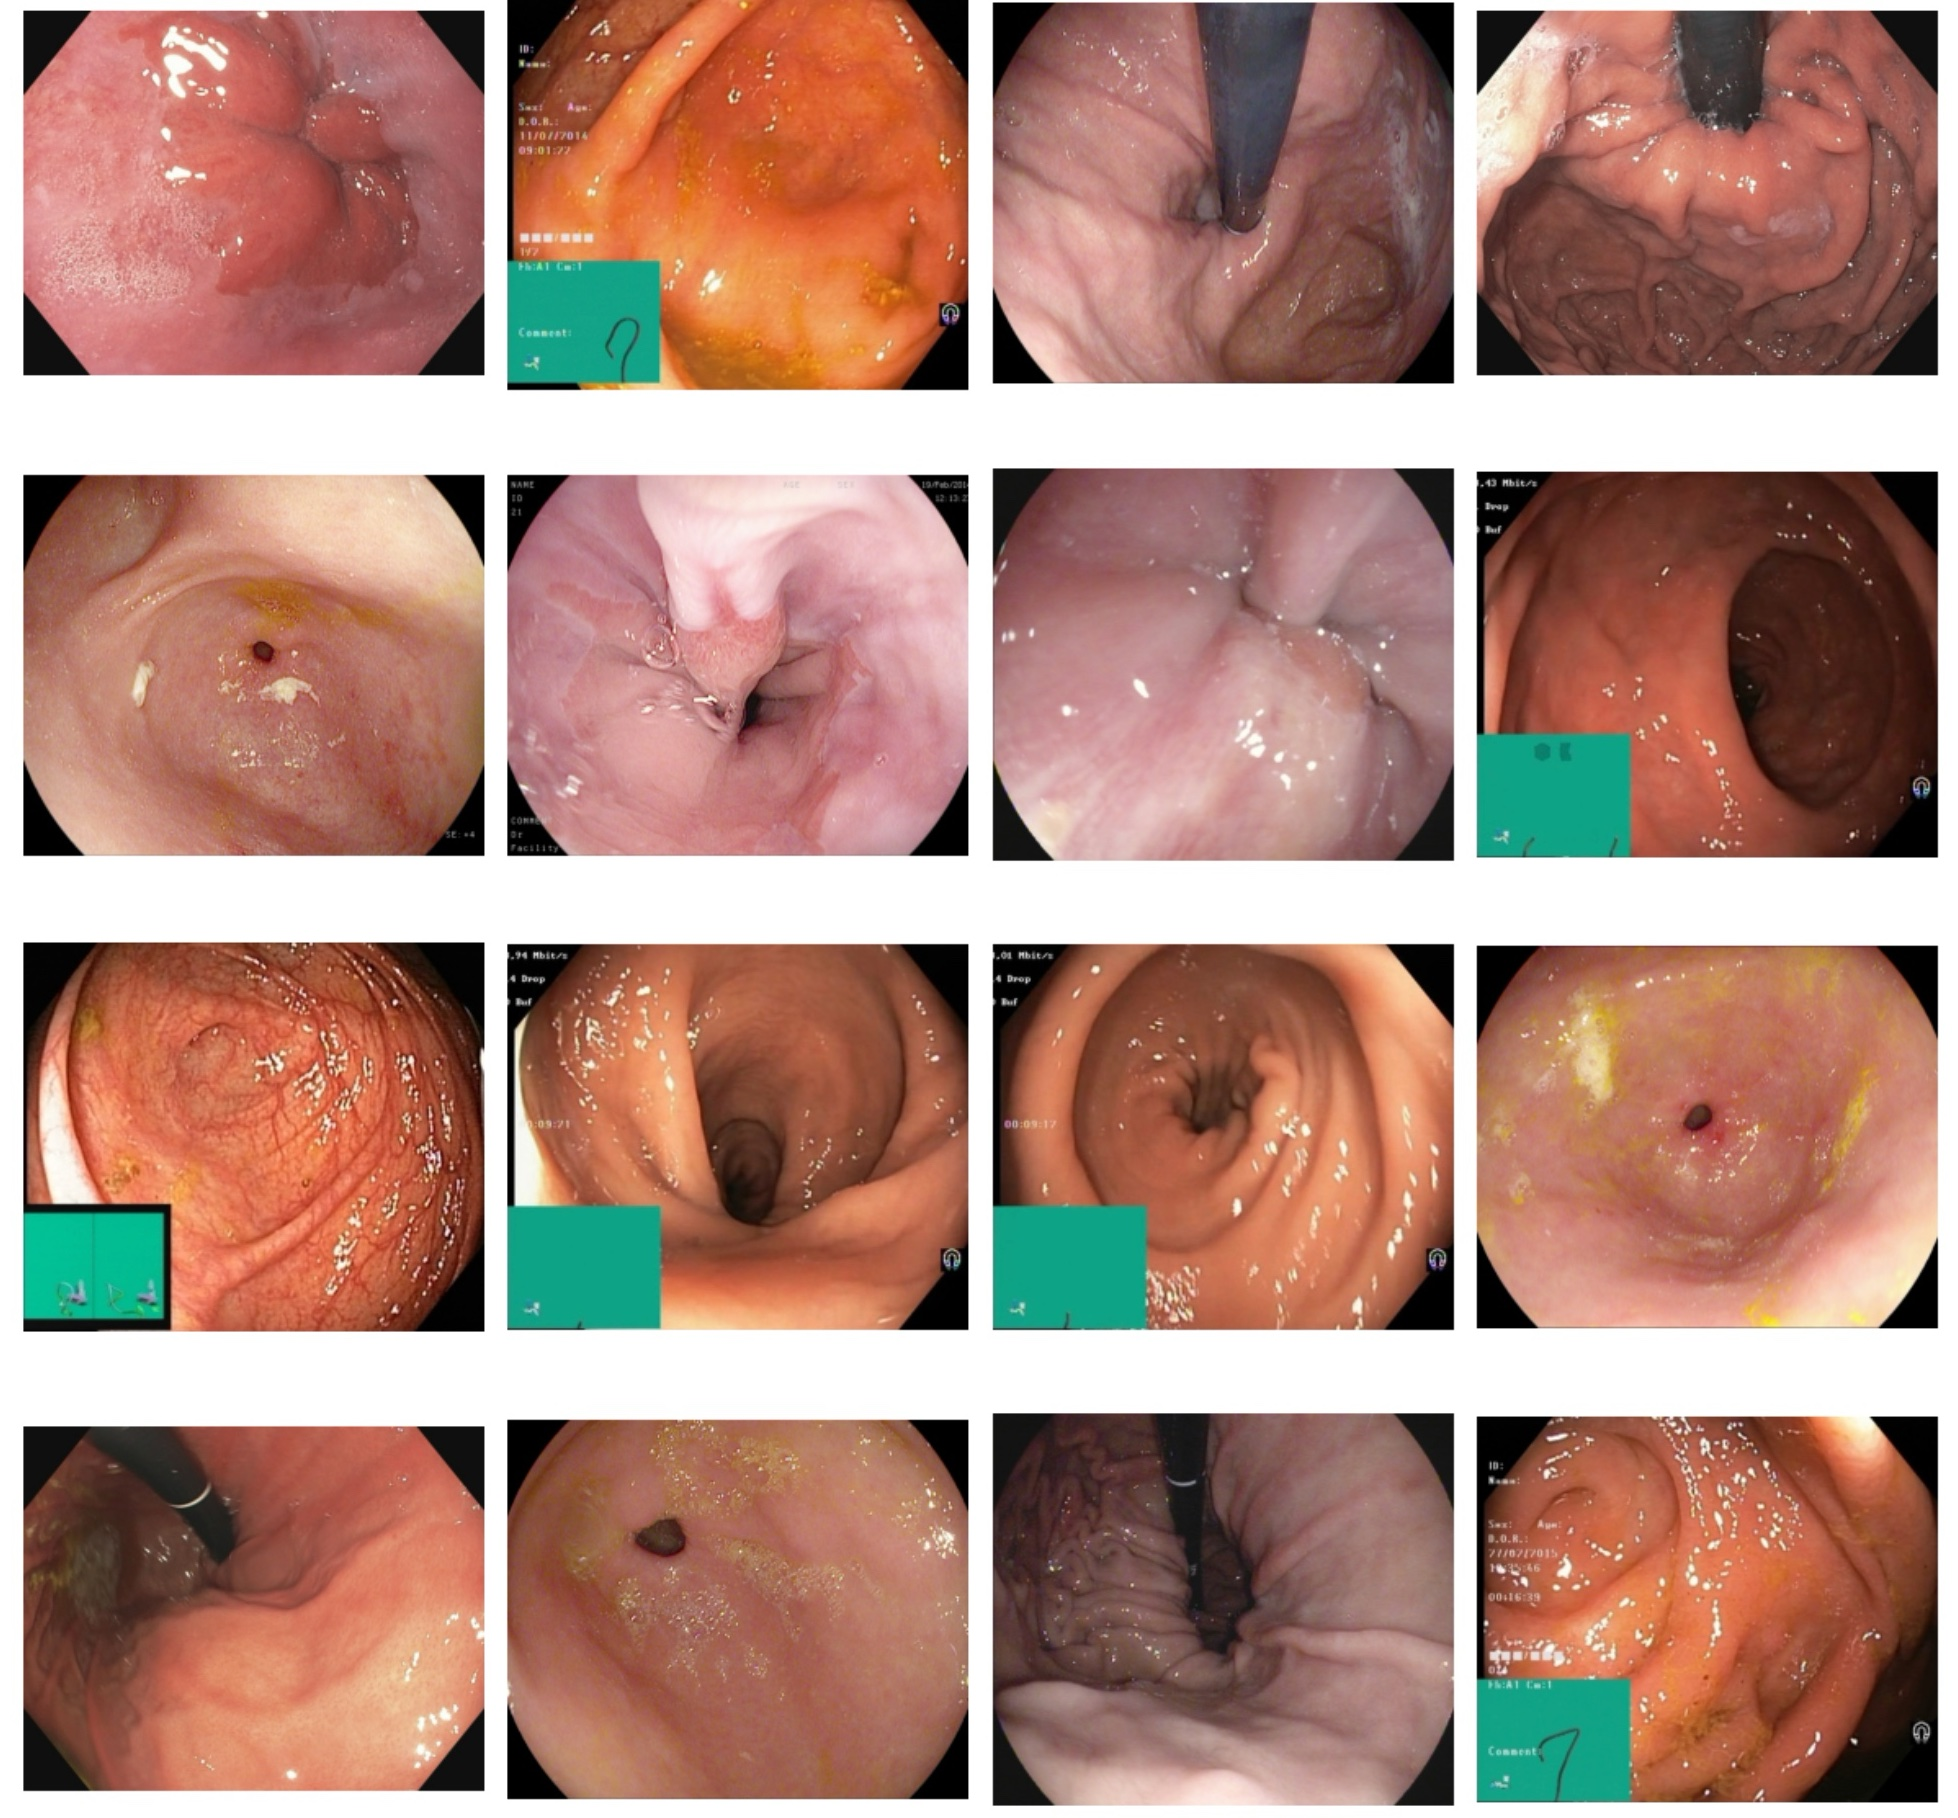
\includegraphics[width=1\textwidth]{Images/Original_Images.jpeg}
    \caption{A sample from the original images from HyperKvasir dataset}
    \label{fig:Original_image}
\end{figure}

\begin{figure}[ht]
    \centering
    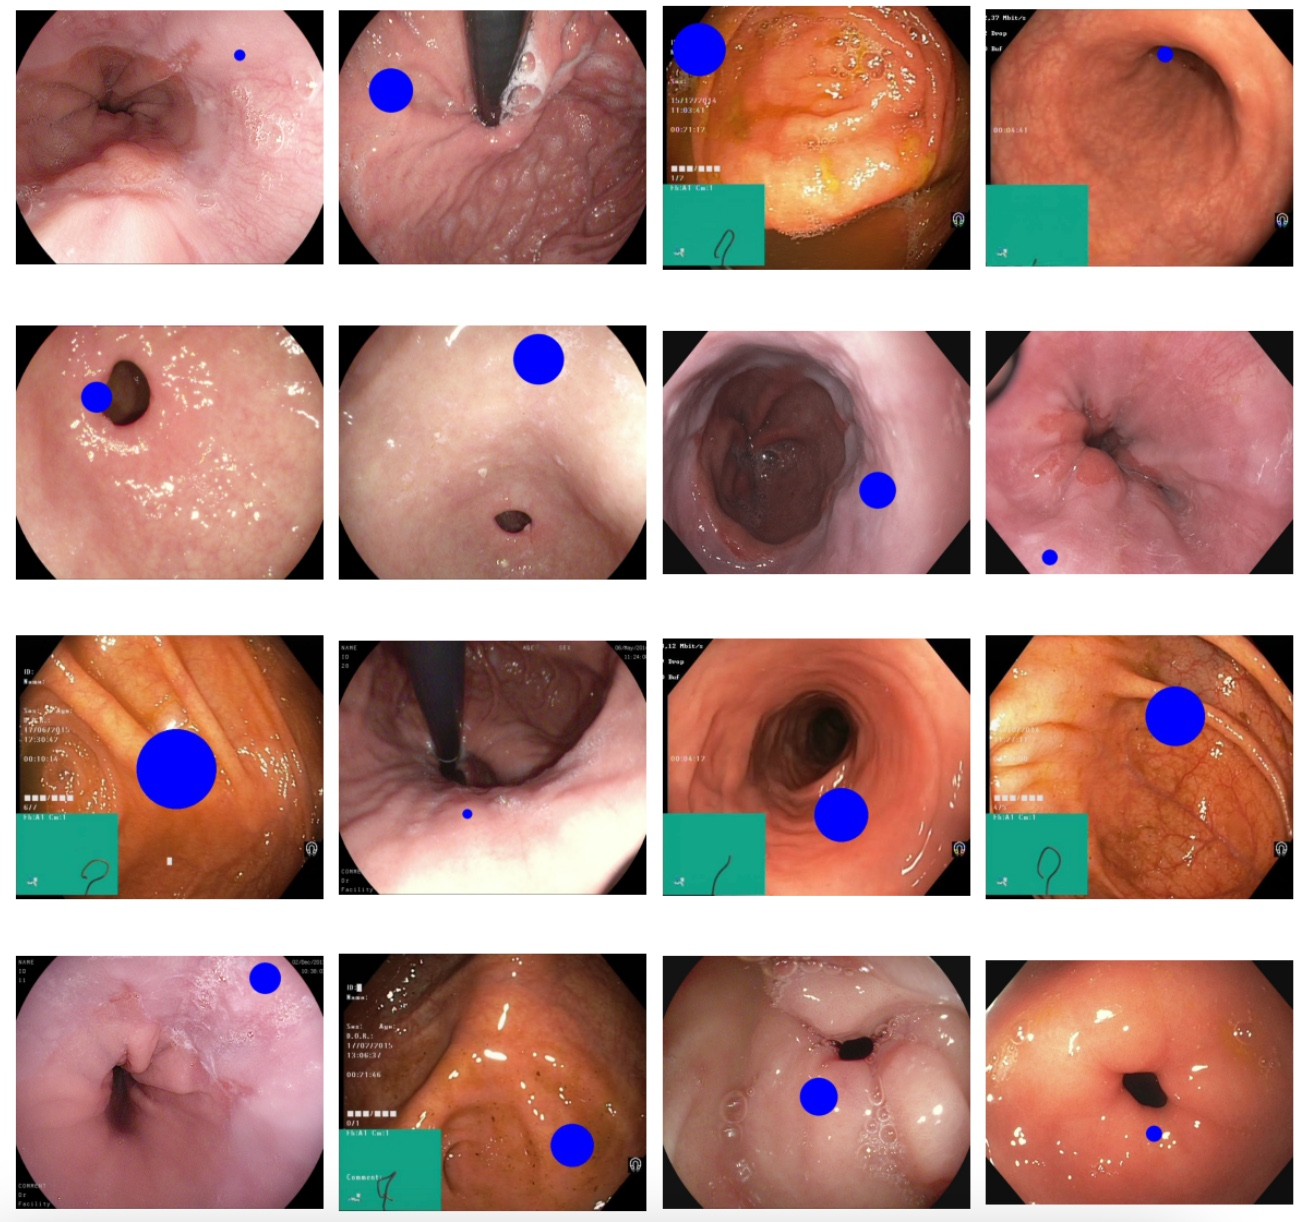
\includegraphics[width=1\textwidth]{Images/Synthetic_images.jpeg}
    \caption{A sample from the synthetic images created by placing blue round shapes on original images from HyperKvasir dataset}
    \label{fig:Synthetic_image}
\end{figure}

For implementing our synthetic data generation process, we follow these steps:
\begin{itemize}
\item Folder Setup: We organize our dataset into two subfolders: "original\_labelled\_images" and "synthetic\_images." The former contains original, labeled images of healthy gastrointestinal tissues, while the latter will store the modified images with synthetic polyps of blue circle.

\item Image Selection: We iterate through the images in the "original\_labelled\_images" folder, selecting each one for augmentation.

\item Synthetic Abnormality Addition: For each selected image, we randomly determine the position and size of a blue circular shape, simulating a polyp. This synthetic abnormality is then superimposed onto the original image.

\item Image Saving: The modified image, now containing the synthetic abnormality, is saved in the "synthetic\_images" folder.
\end{itemize}

The images in the "original\_labelled\_images" and "synthetic\_images" folders serve as domain A and domain B, respectively, for our Image-to-Image (I2I) translation model. During training, the model learns to map and translate images between these two domains, enabling it to generate realistic images of abnormalities from healthy images. In the testing phase, the trained model can generate synthetic images of abnormalities based on unseen healthy images, aiding in the evaluation of its performance.

\section{Preprocessing of Horse2Zebra Dataset}

For image to image translation task, we first start implementing CycleGAN Model on the Horse2Zebra dataset. The dataset is downloaded from \cite{kaggle_horse2zebra_dataset}. This dataset has four subfolders: trainA, trainB, tsetA, testB. A domain represents images of horse and B domain represents images of zebra.

We preprocess the training data by resizing the images to a standard size, performing random cropping, and horizontal flipping to augment the dataset. The preprocessed images are then converted to PyTorch tensors for further processing. The dataset is loaded using a custom ImageDataset class, which reads images from the corresponding directories for horses and zebras. The ImageDataset class loads images from the specified directories and applies the provided transformations such as resizing, cropping, and flipping.

\section{Preprocessing of Hyper Kvasir Dataset}

The Hyper Kvasir dataset serves as the foundation for training and evaluating the Image-to-Image (I2I) translation models using the CycleGAN architecture. Prior to model training, it is essential to preprocess the dataset to ensure uniformity, consistency, and compatibility with the model's input requirements. The preprocessing pipeline involves several key steps:

\textbf{{Dataset Organization:}}
The Hyper Kvasir dataset comprises of labeled image data, unlabeled image data, segmented image data, and annotated video data , totaling 1,11,079 images and 373 videos \cite{HyperKvasir_Dataset}. However, for the thesis, our focus will be on a subset of 6,255 images from the labeled dataset. This subset, denoted as "Original Images" for domain A, will be utilized alongside another set of 6,255 images labeled as "Synthetic Images" for domain B. The Synthetic Images are generated by adding random shapes and sizes of blue circles to the Original Images. These categories represent the source and target domains for the I2I translation task. The dataset is organized into separate directories for original images and synthetic images, facilitating easy access and management during preprocessing and training phases.

\textbf{{Data Loading and Augmentation:}}

Data loading involves the systematic retrieval of image files from their respective directories. The Python glob module is used to recursively search for image files within the respective directories. Each image file is loaded using the Python Imaging Library (PIL), providing necessary functionalities for image manipulation and processing.

To augment the dataset and increase its diversity, data augmentation techniques are applied. These techniques introduce variations in the training samples while retaining their fundamental semantic content.
Augmentation strategies, such as random cropping and horizontal flipping, are used using the torchvision.transforms module. These transformations contribute to enhanced model robustness and generalization capability.

\textbf{{Normalization:}}

Pixel normalization is performed to standardize the pixel values of the images, ensuring uniform input distributions across the dataset. The pixel values are normalized to a range between 0 and 1, followed by scaling to a range between -1 and 1. This normalization scheme aligns with the typical input requirements of neural network models and adds in stabilizing the training process.

\textbf{{Dataset Splitting:}}

The preprocessed HyperKvasir dataset which consist of "Original
Images" and "Synthetic Images" of 6,255 each, is split into training and testing sets. "Original Images" (A domain) is divided into 5,255 images for trainA and 1000 images for testA. "Synthetic Images" (B domain) is divided into 5,255 images for trainB and 1000 images for testB. The training set is used to train the CycleGAN model, while the testing set is used to evaluate the model's performance. 

\textbf{{Data Loader:}}

A data loader object is created to efficiently manage the preprocessed data during training. The data loader shuffles the training data and loads batches of images for feeding into the CycleGAN model.

By following this preprocessing pipeline, the Hyper Kvasir dataset is transformed into a structured and preprocessed format suitable for training the CycleGAN model. The addition of synthetic data, augments the dataset's variability and richness, contributing to improved model performance and translation accuracy. These preprocessing steps lay the foundation for model training and evaluation, ensuring a robust and effective experimental setup.

\section{CycleGAN Model Architecture}

In this section, we are going to discuss Generator model Architechture and summary, Hyperparameters of Generator and Discriminator.  

\subsection*{Generator Architechture:} The generator network comprises several layers including convolutional, instance normalization, rectified linear unit (ReLU), and residual blocks as shown in figure \ref{fig:Generator_architechture} . Each layer plays a crucial role in transforming input images from one domain to another effectively. The architecture consists of contracting blocks followed by several residual blocks which help in preserving the essential features of the input images during the translation process as shown in figure \ref{fig:G_model_summary}. Additionally, expanding blocks are employed to upsample the features to generate the translated output images.
This model summary can be visualised in a graphical generated computation graph as shown in figure \ref{fig:generator_visualization}.
The generator comprises a total of 11,378,179 parameters, all of which are trainable, indicating their adaptability during the training process. There are no non-trainable parameters present in the model as shown in figure \ref{fig:Generator_parameters}. 

\begin{figure}[htbp]
    \centering
    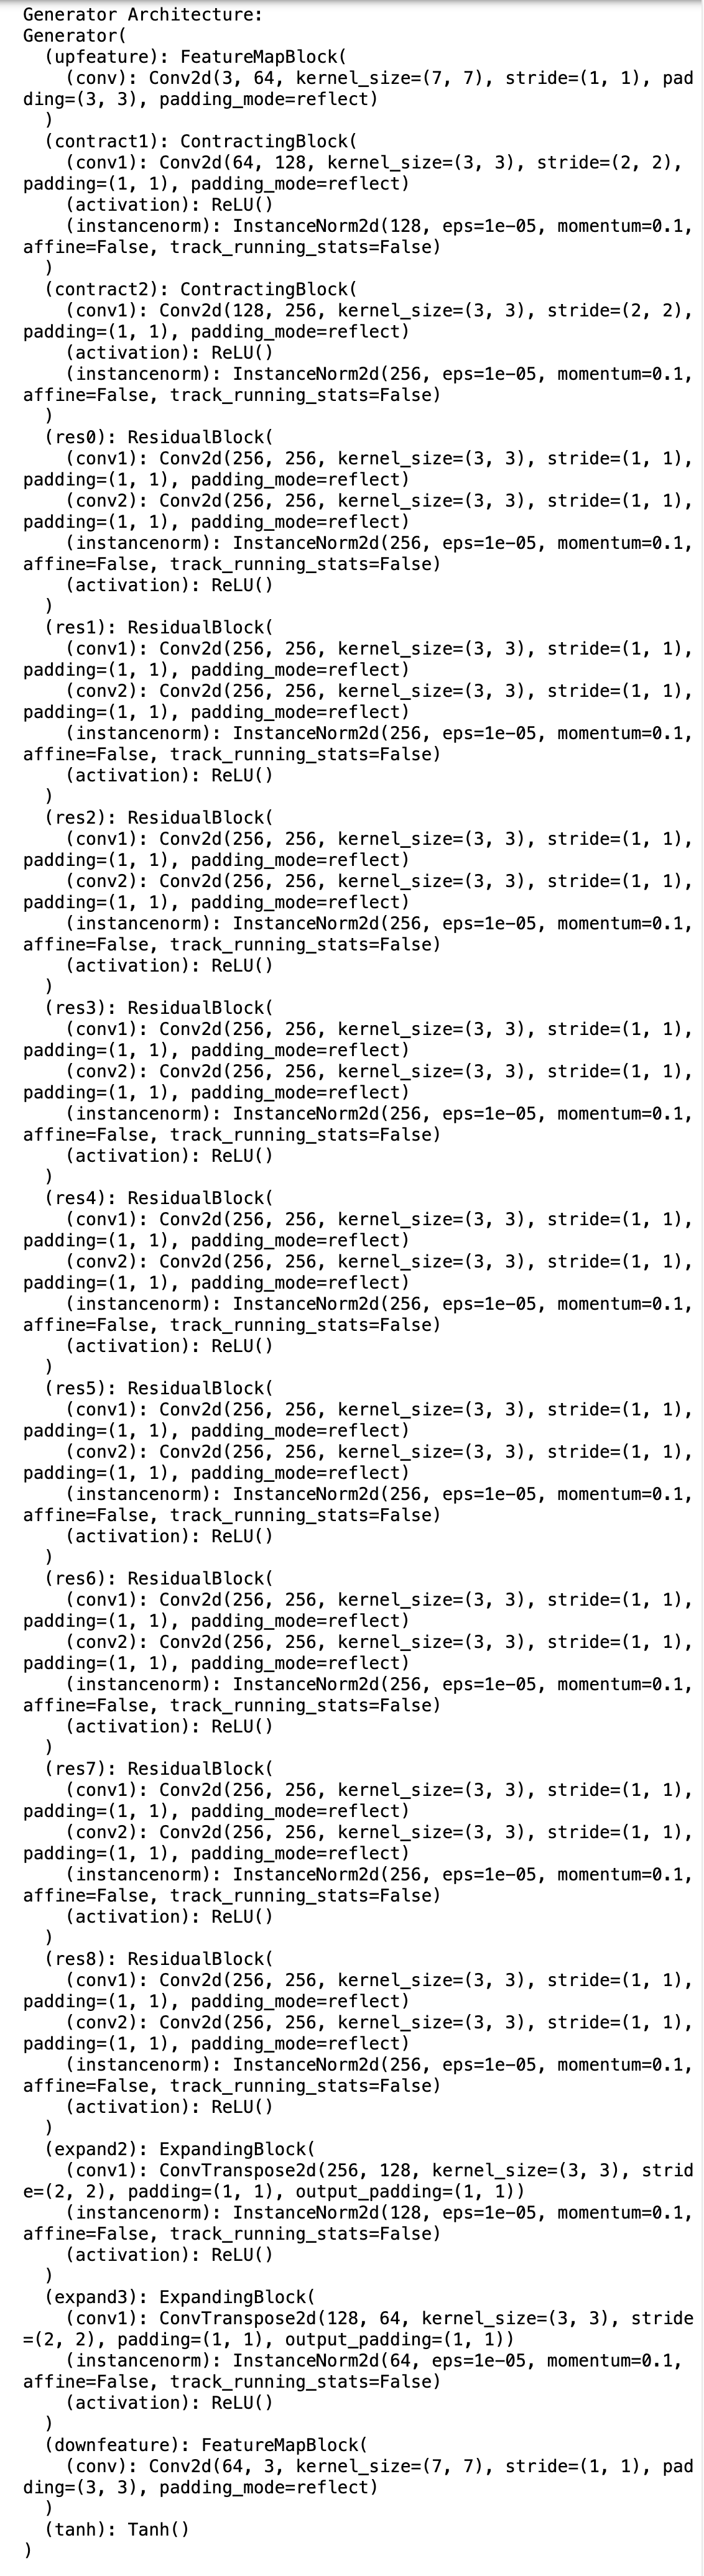
\includegraphics[width=0.4\textwidth]{Images/Generator_architechture.png}
    \caption{Generator model Architechture}
    \label{fig:Generator_architechture}
\end{figure}

\begin{figure}[htbp]
    \centering
    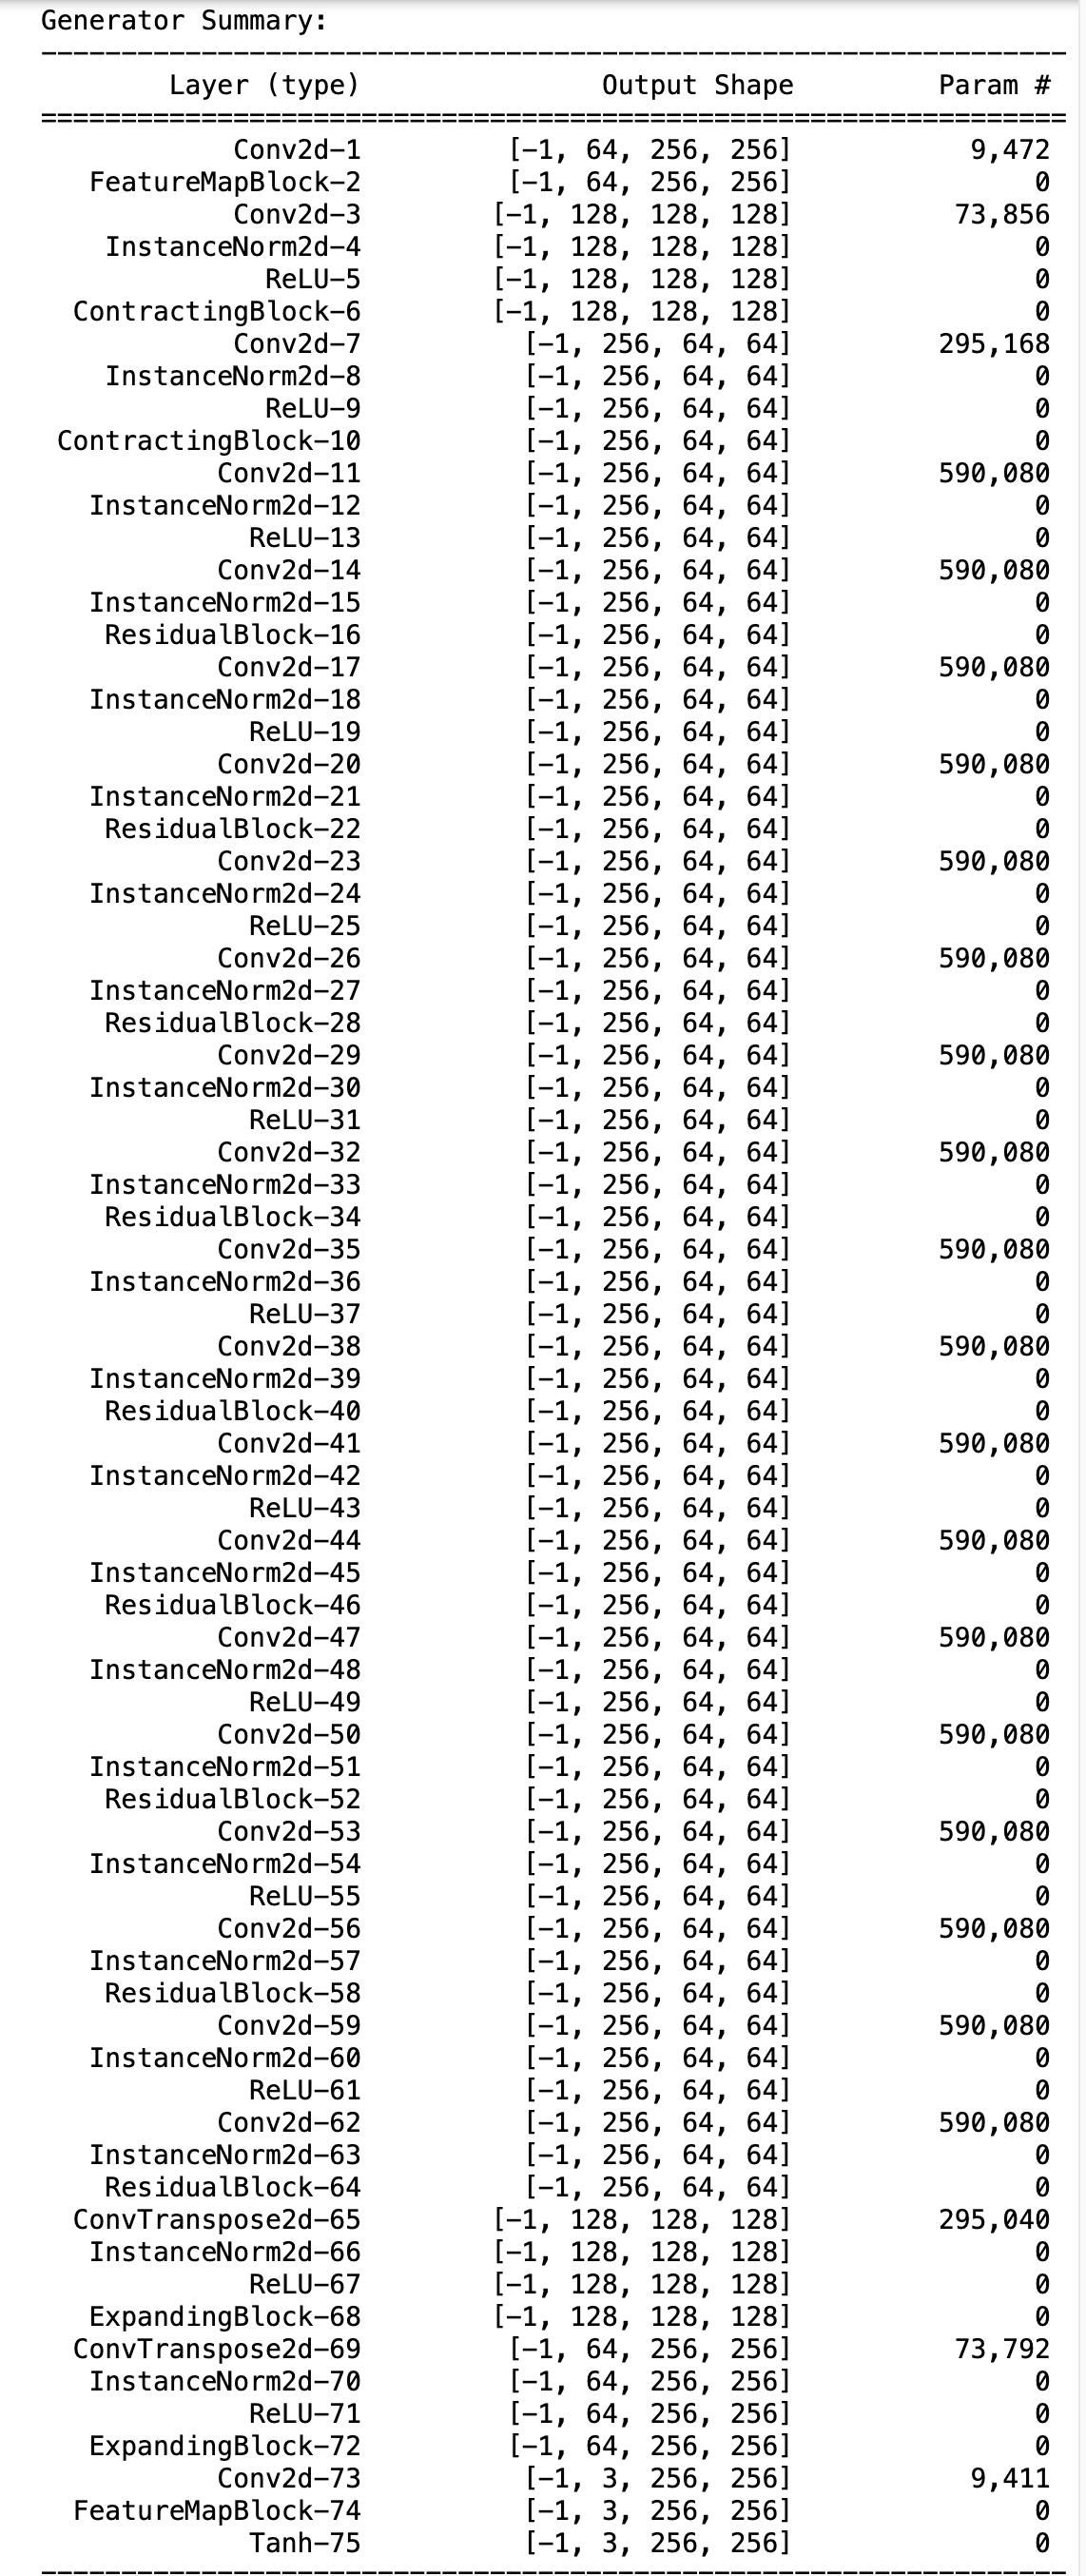
\includegraphics[width=0.6\textwidth]{Images/G_model_summary.png}
    \caption{Generator model summary}
    \label{fig:G_model_summary}
\end{figure}



\begin{figure}[htbp]
    \centering
    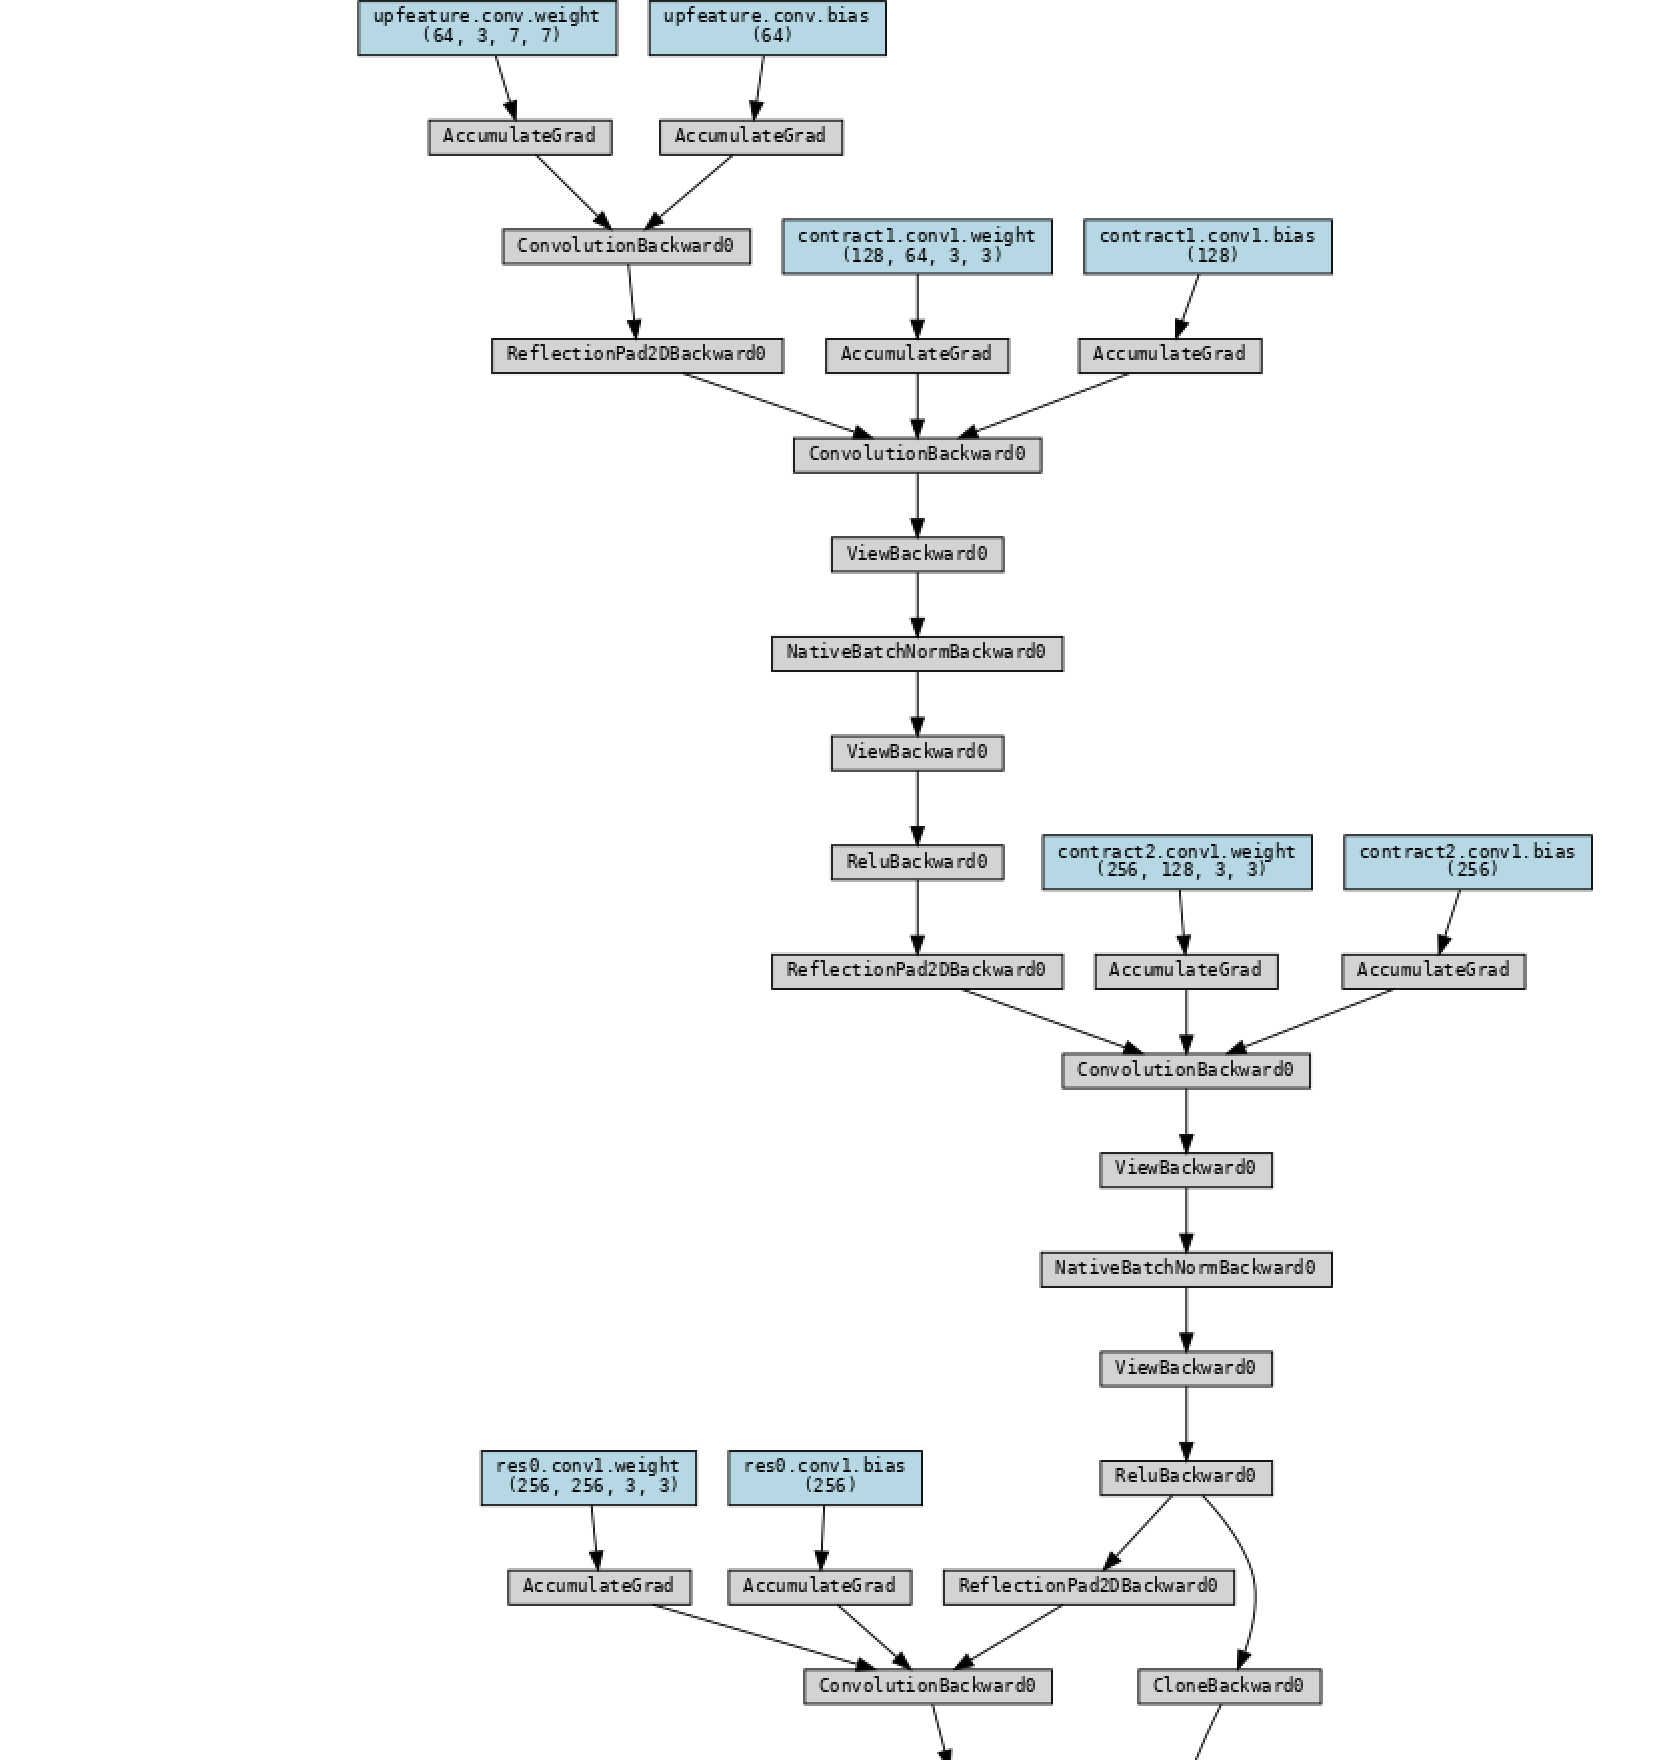
\includegraphics[width=1\textwidth]{Images/generator_visualization.png}
    \caption{Generator model graph}
    \label{fig:generator_visualization}
\end{figure}

\begin{figure}[htbp]
    \centering
    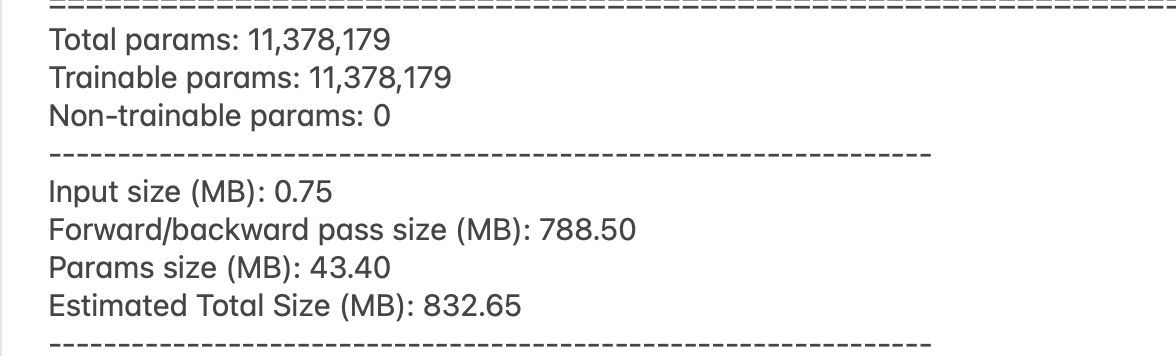
\includegraphics[width=1\textwidth]{Images/Generator_parameters.png}
    \caption{Generator Hyperparameters}
    \label{fig:Generator_parameters}
\end{figure}

\subsection*{Discriminator Architechture:} The discriminator begins with convolutional layers followed by leaky ReLU activation functions, facilitating feature extraction and nonlinear transformations as shown in figure \ref{fig:Discriminator_Architechture}. Contracting blocks are utilized to downsample the feature maps, progressively reducing the spatial dimensions as shown in figure \ref{fig:D_model_summary}. Instance normalization is applied to stabilize the training process and enhance convergence. This model summary can be visualised in a graphical generated computation graph as shown in figure \ref{fig:discriminator_visualization}. The discriminator has 2,763,393 parameters, all of which can be adjusted during training. There are no fixed parameters, showing how flexible the model is as shown in figure \ref{fig:D_parameters}.

\begin{figure}[htbp]
    \centering
    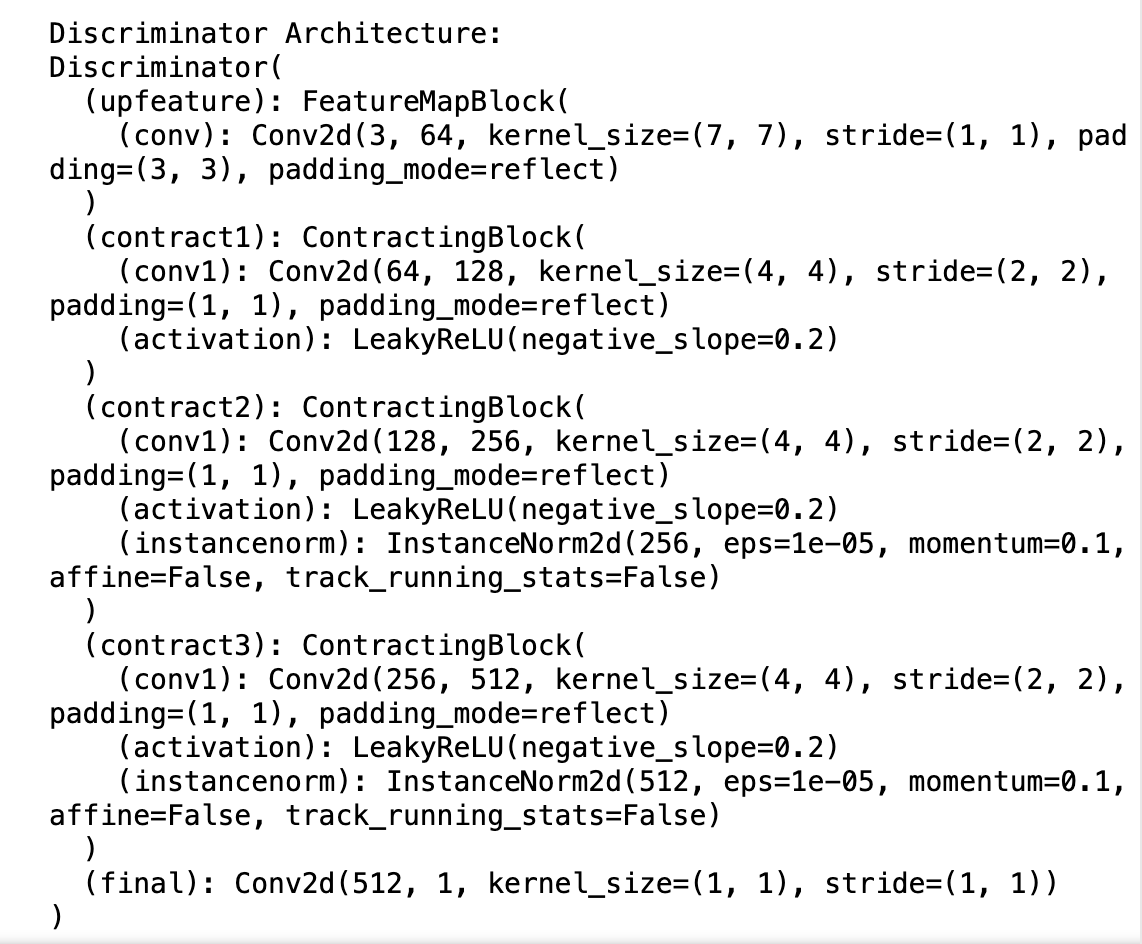
\includegraphics[width=1\textwidth]{Images/Discriminator_Architechture.png}
    \caption{Discriminator model Architechture}
    \label{fig:Discriminator_Architechture}
\end{figure}

\begin{figure}[htbp]
    \centering
    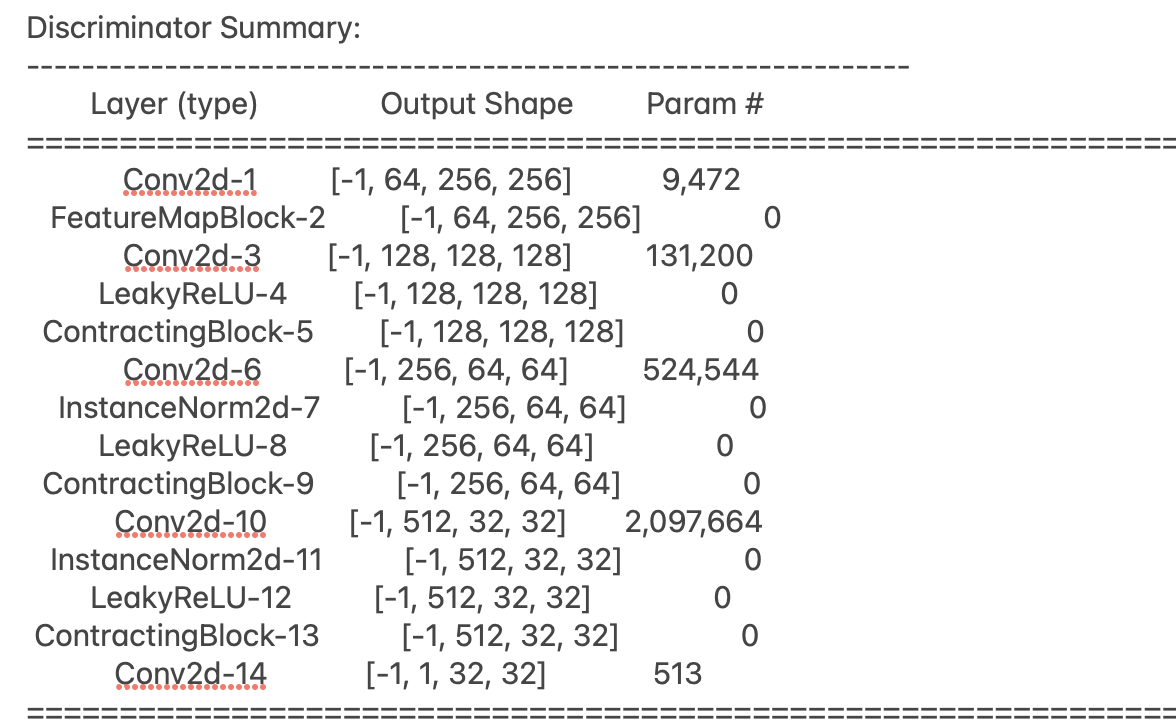
\includegraphics[width=1\textwidth]{Images/D_model_summary.png}
    \caption{Discriminator model summary}
    \label{fig:D_model_summary}
\end{figure}

\begin{figure}[htbp]
    \centering
    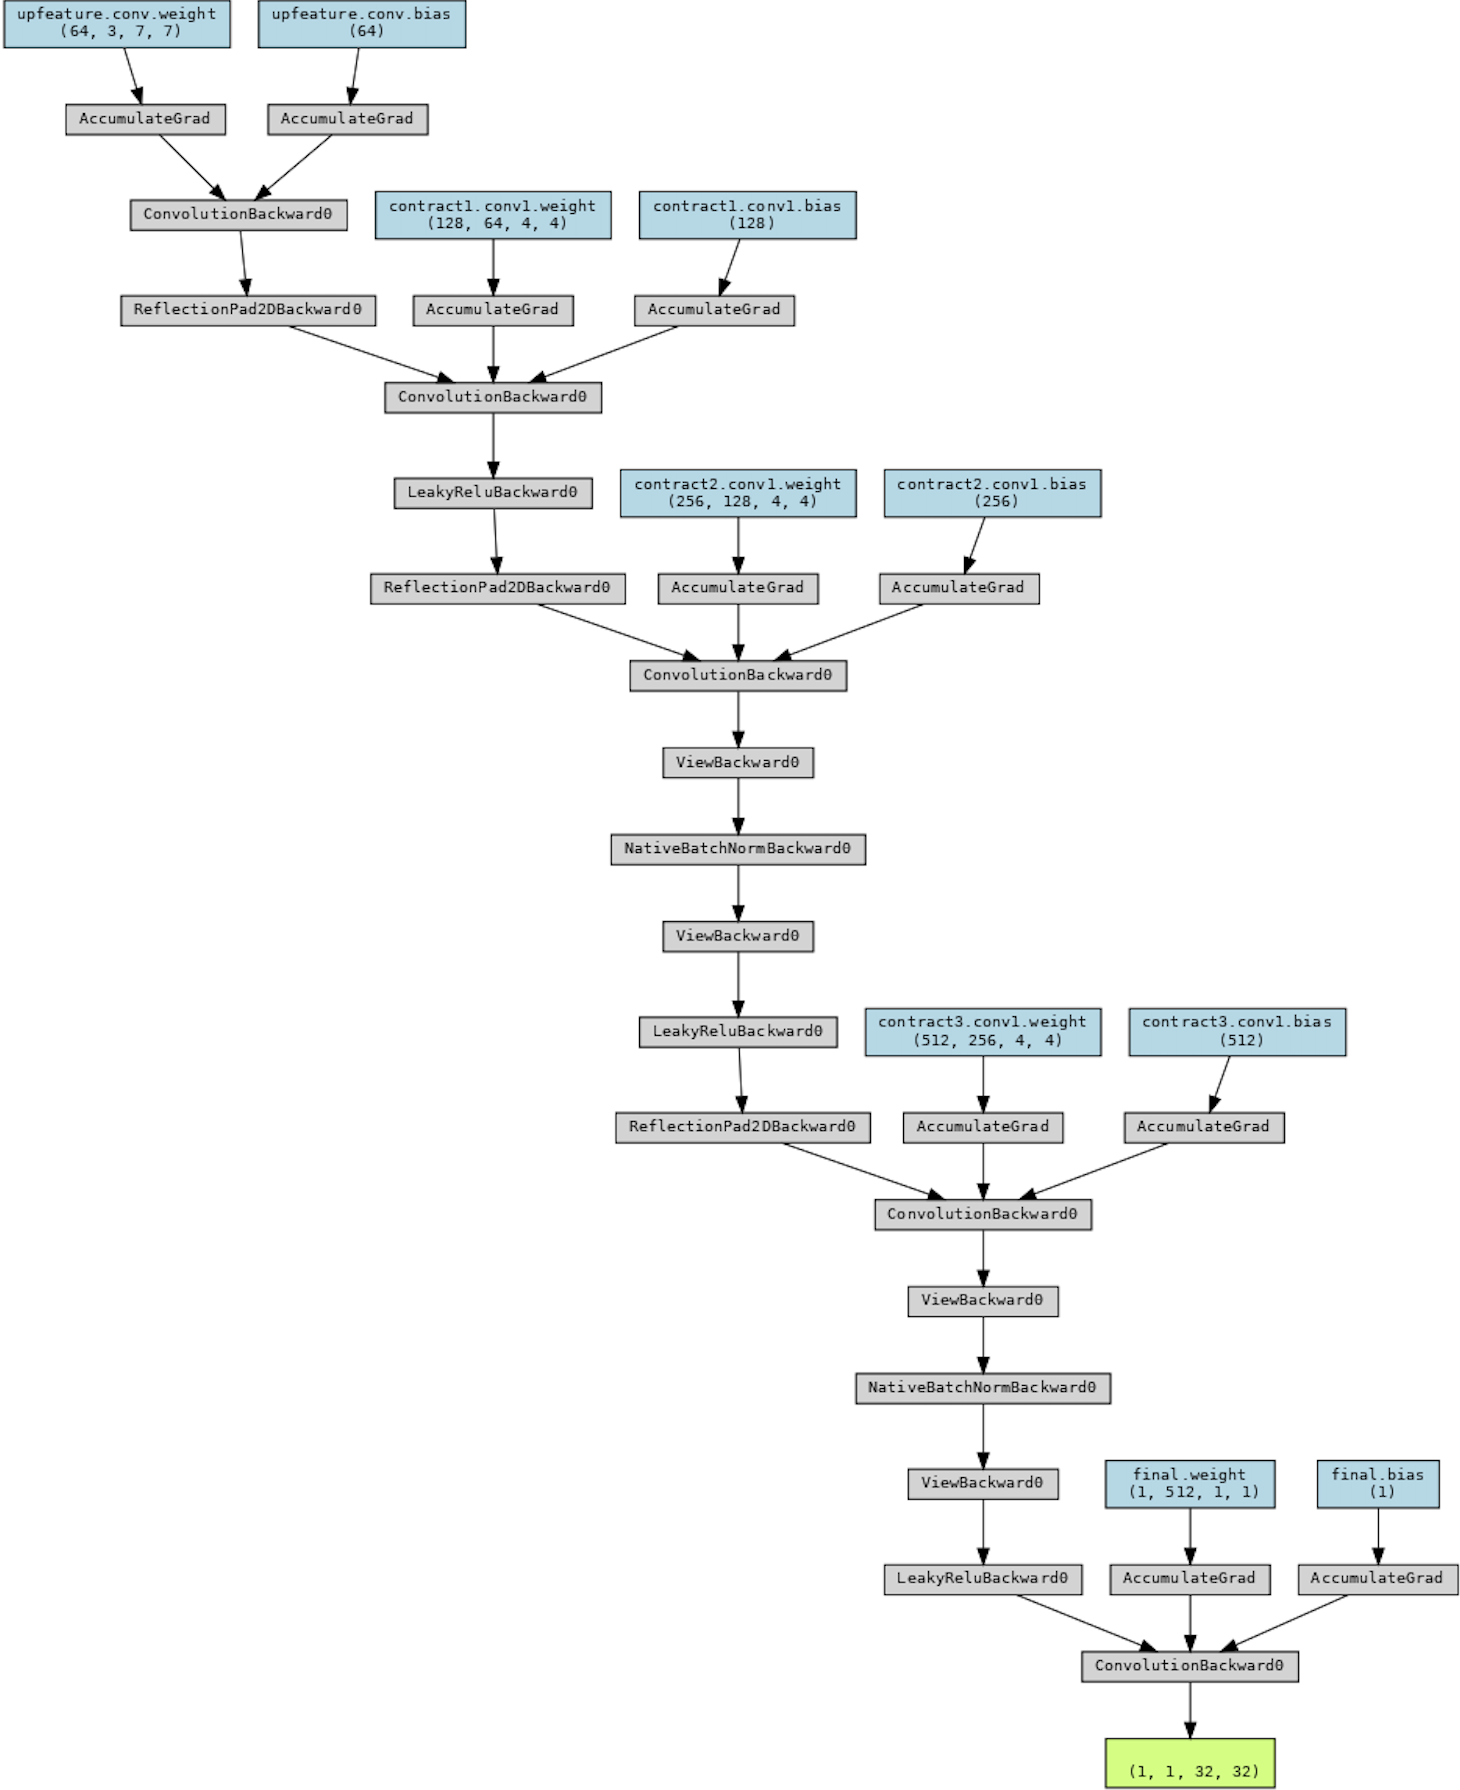
\includegraphics[width=1\textwidth]{Images/discriminator_visualization.png}
    \caption{Discriminator model graph}
    \label{fig:discriminator_visualization}
\end{figure}


\begin{figure}[htbp]
    \centering
    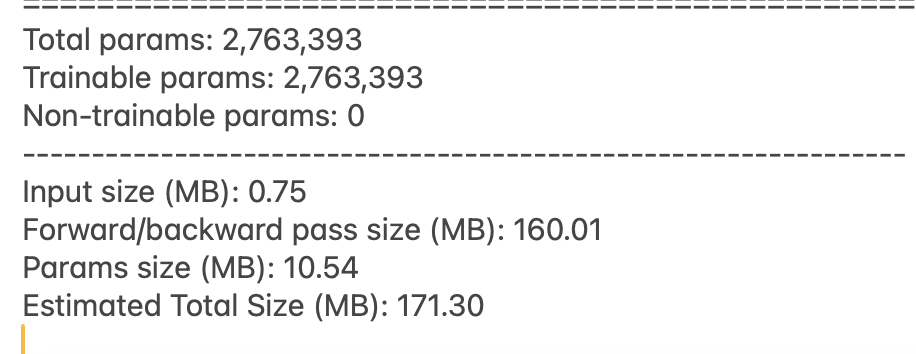
\includegraphics[width=1\textwidth]{Images/D_parameters.png}
    \caption{Discriminator Hyperparameters}
    \label{fig:D_parameters}
\end{figure}

\section{Image-to-Image translation using CycleGAN}

For the I2I translation task, we employed the CycleGAN model \cite{CycleGAN}. The CycleGAN model is designed to establish mapping functions between two distinct domains (A and B) without relying on paired images as input, thus enabling unsupervised I2I translation. Given two sets of unpaired image inputs from different domains (e.g., healthy images and synthetic images), the model employs a Generator (G) to map images from one domain to the other. Concurrently, a Discriminator network (D) is constructed to differentiate between real and generated (fake) images. The Generator and Discriminator are trained as adversaries, with the Generator aiming to deceive the Discriminator into believing that its generated images are real.

To enhance the consistency and preserve image features during translation, a cycle consistency loss is calculated. This loss function \cite{CycleGAN} ensures that the translated images can be converted back to their original domain and closely match the initial input images. Additionally, an identity loss is calculated to evaluate the model's ability to accurately understand the domain of the input image. Specifically, when an image from the target domain is provided as input, the Generator network is expected to make minimum or no alterations to it, preserving its original characteristics. The architecture of the network, along with the cycle and identity losses. This framework demonstrates the comprehensive method adopted by the CycleGAN model for unsupervised I2I translation, highlighting the incorporation of adversarial training, cycle consistency, and identity preservation to achieve high-quality image synthesis across different domains.

\section*{Implementation Overview}

In this section, we explain the methodology used for Image-to-Image (I2I) translation using the CycleGAN framework, along with observation done from implementing the model on various datasets. Our method for Image-to-Image translation utilizes CycleGAN architecture, which learns mappings between two domains without paired training data. We employed PyTorch to implement the CycleGAN model \cite{CycleGAN}, referencing existing GitHub repositories for guidance during implementation.


\section*{GitHub Repositories and Model Implementation}

We implemented the CycleGAN model using the PyTorch deep learning framework. Our implementation benefited from insights and code structures obtained from various publicly available repositories on GitHub:
\begin{itemize}
\item Repository 1: Unpaired-Image-To-Image-Translation-CycleGAN (\url{https://github.com/Mananp96/Unpaired-Image-To-Image-Translation-CycleGAN}): This repository provided a foundational understanding of CycleGAN architecture and its implementation using PyTorch.
\item Repository 2: pytorch-unpaired-image-to-image-translation (\url{https://github.com/kiyohiro8/pytorch-unpaired-image-to-image-translation}) : This repository offered a more comprehensive implementation of CycleGAN, including training scripts and loss functions, which aided in building a robust model.
\item Repository 3: pytorch-GANs/Apply Generative Adversarial Networks (\url{https://github.com/furkannturkmen/pytorch-GANs/tree/main/Apply%20Generative%20Adversarial%20Networks}):  This repository served as a general reference for understanding Generative Adversarial Networks (GANs), the core concept upon which CycleGAN is built.
\end{itemize}

\section*{Training Procedure}

The training procedure for this thesis involves several key steps, including model initialization, optimization, and evaluation. The following sections outline the detailed training procedure:

\subsection*{1. Model Initialization}

The CycleGAN model consists of two generator networks (Generator A-to-B and Generator B-to-A) and two discriminator networks (Discriminator A and Discriminator B). The generator networks (Generator) are responsible for translating images from one domain to another, while the discriminator networks (Discriminator) aim to distinguish between real and translated images. Additionally, the model includes auxiliary modules such as ResidualBlock, ContractingBlock, ExpandingBlock, and FeatureMapBlock, which are building blocks used within the generator and discriminator architectures \cite{CycleGAN} .
\begin{itemize}
\item \textbf{ResidualBlock:}
The ResidualBlock class represents a fundamental building block within the generator architecture. Its purpose is to facilitate the learning of residual mappings, allowing for more efficient training and enhanced feature extraction. During training, the ResidualBlock is instrumental in preserving the high-frequency details and fine-grained information of the input images \cite{CycleGAN} . By incorporating residual connections, it enables the generator network to effectively capture and propagate useful information across multiple layers, contributing to improved translation accuracy and image quality.

\item \textbf{ContractingBlock:}
The ContractingBlock class plays an important role in downsampling and feature extraction within the generator architecture. By applying convolutional operations followed by activation functions, the ContractingBlock effectively reduces the spatial dimensionality of the input feature maps while increasing the number of channels. This process enhances the model's ability to capture hierarchical features and spatial dependencies within the input images. During training, the ContractingBlock facilitates the extraction of abstract representations from the input images, enabling the generator network to learn meaningful transformations and generate realistic translations \cite{CycleGAN} .

\item \textbf{ExpandingBlock:}
The ExpandingBlock class serves as the counterpart to the ContractingBlock within the generator architecture, responsible for upsampling and feature expansion. Through transposed convolutional operations and activation functions, the ExpandingBlock increases the spatial resolution of the feature maps while reducing the number of channels. This process facilitates the reconstruction of high-resolution output images from the abstract representations learned by the generator network. During training, the ExpandingBlock aids in recovering fine-grained details and structural information lost during the downsampling process, ensuring the fidelity of the generated images \cite{CycleGAN} .

\item \textbf{FeatureMapBlock:}
The FeatureMapBlock class represents the final layer of the generator network, responsible for mapping the feature maps to the desired number of output channels. By applying convolutional operations, the FeatureMapBlock adjusts the channel dimensionality of the feature maps to match the desired output format. During training, the FeatureMapBlock consolidates the learned representations into the final output images, preparing them for further processing or evaluation. Additionally, the FeatureMapBlock contributes to regularization and stabilization during training, helping to mitigate overfitting and improve generalization performance \cite{CycleGAN} .

\item \textbf{Generator:}
The Generator class encapsulates the entire generator network architecture within the CycleGAN model. Comprising upfeature, contracting, residual, expanding, and downfeature blocks, the Generator orchestrates the transformation of input images from one domain to another. During training, the Generator leverages the aforementioned blocks to learn the mapping between the original labeled and synthetic image domains. By iteratively refining the generated outputs through the application of residual connections and feature extraction operations, the Generator facilitates the generation of high-quality translations with enhanced realism and fidelity \cite{CycleGAN} .

The Generator class implements the U-Net architecture. It consists of contracting blocks, residual blocks, and expanding blocks. The contracting blocks reduce the spatial dimensions of the input, while the expanding blocks upsample the feature maps. Residual blocks help in preserving image details during the transformation process [27] . The generator takes images from one domain (e.g. original healthy images) and transforms them into images from the other domain (e.g.synthetic images)

\item \textbf{Discriminator:}
The Discriminator class represents the discriminator network within the CycleGAN model, tasked with discriminating between real and fake images. Comprising upfeature and contracting blocks, along with a final convolutional layer, the Discriminator learns to distinguish between authentic images from the original labeled domain and synthesized images from the generator network. During training, the Discriminator provides adversarial feedback to the generator network, guiding it towards generating more realistic translations. By iteratively updating its parameters based on the discriminator's feedback, the generator network learns to produce images that are indistinguishable from genuine samples \cite{CycleGAN} .

The Discriminator class is structured similar to the contracting path of a U-Net. It takes an input image and outputs a matrix of values classifying different portions of the image as real or fake. The discriminator is trained to distinguish between real images from the target domain and fake images generated by the
generator.
\end{itemize}


\subsection*{2. Optimization Setup:}
The optimization process involves defining the loss functions, selecting optimization algorithms, and setting hyperparameters. Adversarial loss (MSELoss) and reconstruction loss (L1Loss) are commonly used for CycleGAN training \cite{CaGAN} . Adversarial loss measures the ability of the generators to generate realistic images, while reconstruction loss encourages cycle-consistency between the original and translated images.
The Adam optimizer (torch.optim.Adam) is typically employed for training both the generator and discriminator networks. It offers adaptive learning rates and momentum parameters, facilitating efficient optimization.

\subsection*{3. Data Loading and Batch Processing:}
The preprocessed dataset is loaded using data loaders (DataLoader), which provide functionalities for batching, shuffling, and parallel data loading. During training, data batches consisting of paired images from the original labeled and synthetic categories are fed into the model.

\subsection*{4. Model Training:}

The training loop iterates over the dataset for a specified number of epochs, with each iteration comprising three steps. The "Forward Pass" step where the input images are passed through the generator networks to produce translated images. The "Discriminator Update" step where the discriminator networks are updated to distinguish between real and fake images from both domains. The "Generator Update" step where the generator networks are updated to minimize the adversarial and reconstruction losses, encouraging realistic image generation and cycle-consistency.

The training procedure for the CycleGAN model involves iterating over the dataset for a predefined number of epochs while updating the generator and discriminator networks. Periodically during training, images from both domains (real and fake) are displayed to monitor the progress of the model. The training procedure involves iteratively updating the parameters of the generator
and discriminator networks.
\begin{itemize}
\item Discriminator Training: The discriminators (disc\_A and disc\_B) are trained separately using adversarial loss to distinguish between real and fake images from their respective domains. Fake images are generated by passing real images through the respective generator (gen\_BA for domain A and gen\_AB for domain B). Adversarial loss is calculated using a mean squared error loss function (adv\_criterion).
\item Generator Training: The generators (gen\_AB and gen\_BA) are trained jointly with the discriminators frozen. Adversarial loss is computed for both generators based on the output of the discriminators when presented with generated images. Additionally, identity loss and cycle-consistency loss are calculated to enforce consistency and preserve image characteristics during translation. The total generator loss is a combination of adversarial loss, identity loss, and cycle-consistency loss, each weighted by corresponding lambda values (lambda\_identity and lambda\_cycle). The trained model is saved as "cycleGAN\_cur\_step.pth", which is then loaded and visualised at later stage.
\end{itemize}


\subsection*{5. Model Saving and Checkpointing:}

During training, model checkpoints is periodically saved at every 200 step to disk to ensure the availability of trained models for later use. After completing 100 iterations, the model produces the final output as cycleGAN\_HK\_41800.pth. Checkpointing allows for resuming training from a specific iteration, performing model inference, or fine-tuning the model on new datasets. This model is then loaded later on, for teh testing and evaluating the models performance.

\subsection*{5. GPU framework}

For the training of cycleGAN model, the Simula GPU cluster has been utilized. Access to the NVIDIA-SMI as shown in the \ref{fig:GPU} interface provided the necessary platform to manage and monitor GPU resources, allowing us to optimize performance and track progress during training.
 
\begin{figure}[htbp]
    \centering
    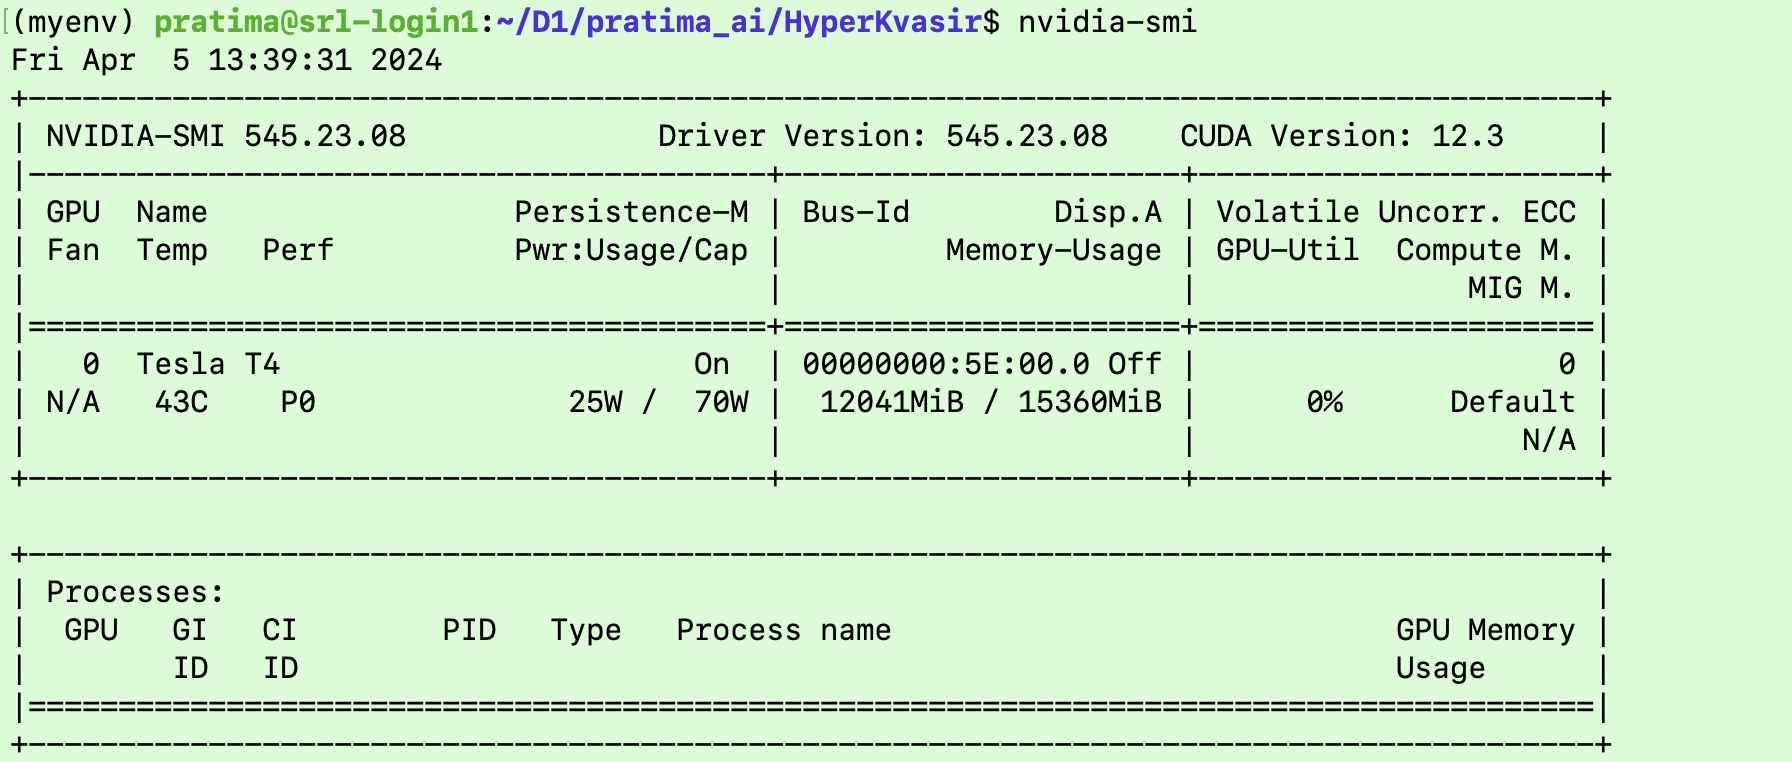
\includegraphics[width=1\textwidth]{Images/GPU.png}
    \caption{NVIDIA GPU}
    \label{fig:GPU}
\end{figure}

To prepare the environment for training, the softwares were meticulously configured by installing essential packages and dependencies using Conda. This included PyTorch, torchvision, torchaudio, and cudatoolkit, all tailored to the specific CUDA version (12.3) supported by the GPU cluster. By aligning software versions with hardware specifications, compatibility and maximized utilization of GPU resources is ensured.

\begin{figure}[htbp]
    \centering
    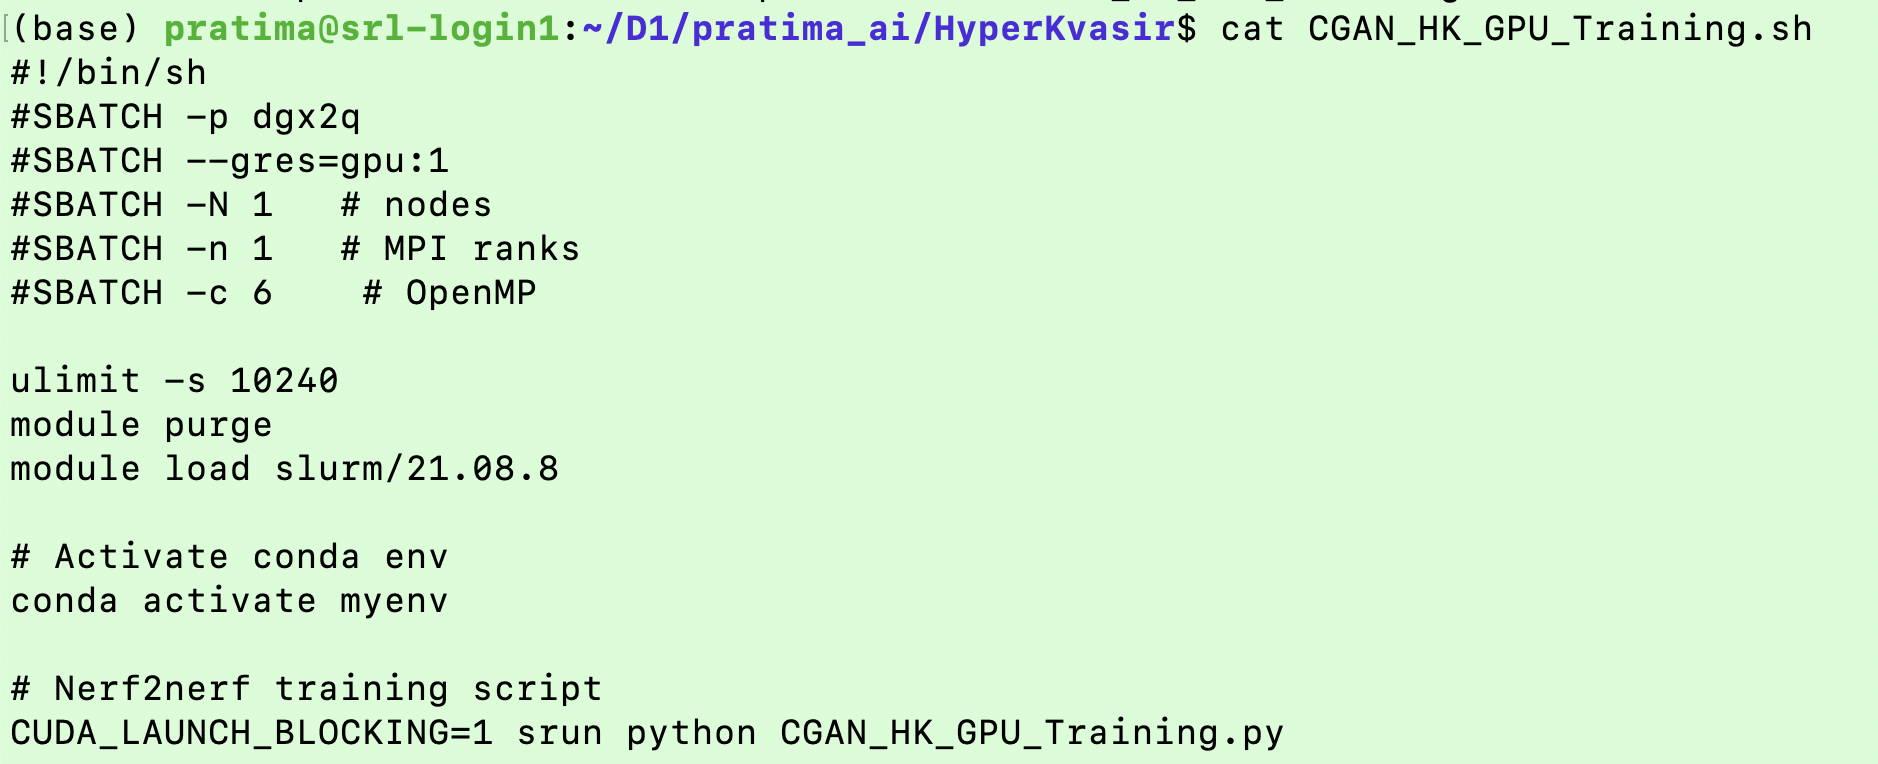
\includegraphics[width=1\textwidth]{Images/sbatch.png}
    \caption{shell script for training the model on GPU cluster}
    \label{fig:sbatch}
\end{figure}

The workflow was further streamlined through the implementation of Python and shell scripts. A Python script (.py file) was developed to package the model training code, serving as the input parameter for the shell script as shown in the \ref{fig:sbatch} responsible for job submission to the GPU cluster using the sbatch command. This automation facilitated the execution of model training , enabling seamless parallel processing and efficient resource allocation across multiple GPUs.

For model evaluation and analysis, I utilized Jupyter notebooks, using their interactive and visual capabilities. By establishing a remote connection to the Simula GPU cluster, I could access and visualize the model outputs in real-time, enabling instant analysis and interpretation of results. This integrated approach to training and testing allowed for iterative experimentation and exploration of the generative properties of Image-to-Image translation methods, laying the foundation for in-depth investigation in my master thesis.

\subsection*{6. Hyperparameters and optimization:}

This section details the hyperparameters and optimization techniques employed for training the CycleGAN model. Selecting appropriate hyperparameters is crucial for effective model training and achieving optimal performance. Through careful
selection and fine-tuning of hyperparameters, along with appropriate optimization techniques, we aimed to achieve efficient training and better performance of the CycleGAN model on the Hyper Kvasir dataset. To optimize the model parameters, the Adam optimizer is employed, with specific learning rates and betas configured for each optimizer (gen\_opt, disc\_A\_opt, and disc\_B\_opt). Additionally, the weights of the model are initialized using a custom weight initialization function to facilitate stable training and convergence. 

Below, we discuss the key hyperparameters and optimization techniques employed in our experimental setup: 
\begin{itemize}
\item Epochs (n\_epochs): This hyperparameter determines the number of times the entire training dataset is passed through the network. A larger number of epochs often leads to better model performance but can also increase training time. For our training, this value is set to 100.
\item Batch Size (batch\_size): The batch size defines the number of images processed by the model in a single training iteration. A larger batch size can improve training efficiency by utilizing more data per update but may also require more computational resources. For our training, we uses a batch size of 10.We started with different batch sizes to find a balance between efficiency and performance on our GPU cluster and dataset.
\item Learning Rate (lr): The learning rate controls the magnitude of the updates made to the model's weights during training. A high learning rate can lead to faster learning but may also cause the model to become unstable or converge to suboptimal solutions. Conversely, a very low learning rate can lead to slow training progress. We use a learning rate of 0.0002. 
\item Image Dimensions (dim\_A, dim\_B): These hyperparameters define the number of color channels in the input and output images. For our training, both dim\_A and dim\_B are set to 3, indicating RGB images.
\item Image Load and Target Shapes (load\_shape, target\_shape): These hyperparameters control the image resizing applied during data preprocessing. Images are initially loaded at a larger size (load\_shape) and then randomly cropped to a smaller target size (target\_shape) before being fed into the network. For our training, load\_shape is set to 286 and target\_shape is set to 256.
\item Optimization Technique: The Adam optimizer is employed to update the weights of both the generators and discriminators during training. Adam is an adaptive learning rate optimization algorithm that considers the historical gradients to adjust learning rates for each parameter individually. This can be particularly beneficial for training deep neural networks with a large number of parameters.

Our model utilizes the Adam optimizer with the following parameters: Beta 1 (0.5) is choosen to exponential decay rate for the first moment estimate of the gradient. Beta 2 (0.999) is choosen to exponential decay rate for the second moment estimate of the gradient (used for variance correction).
\item Weight Initialization: The model utilizes the weights\_init function to initialize the weights of the generators and discriminators with a normal distribution (mean 0, standard deviation 0.02). This helps us to break symmetry in the initial weights and encourages the network to learn more effectively.
\end{itemize}


\chapter{Result}

We first implemented our model on Horse2Zebra dataset for our experimentation and validation of our python code for the cycleGAN model. Then the model was tested, and the output images were produced, which we are going to presnt in this chapter. Then we implemented the model on our HyperKvasir dataset. The models evaluations and performance was analyzed and presented in this chapter.

\section{Generated Images on Horse2Zebra Dataset:}

The CycleGAN model was trained for 20 epochs on Horse2Zebra dataset and model checkpoint was saved as cycleGAN\_21200.pth.  The trained CycleGAN model is tested on "testA" folder having horse images and "testB" folder having zebra images, in Horse2Zebra dataset for image-to-image translation. The model is loaded from the saved checkpoint file (cycleGAN\_21200.pth for this model), and its components are inspected to ensure proper loading. Two generator models, G\_A and G\_B, responsible for translating images from domain A to domain B and vice versa, are initiated and loaded with the corresponding state dictionaries from the checkpoint. The generators are then set to evaluation mode to disable any training-specific operations like dropout.

Image transformations are defined using the torchvision library to resize, convert to tensors, and normalize the images. Test images from the "testA" and "testB" folders of the Horse2Zebra dataset are loaded, and directories are created to store the generated images. The model is tested by iterating through the images in the test sets. Each image is loaded, preprocessed, and passed through the corresponding generator to obtain the translated image. The translated images are then saved in the respective directories. Progress is displayed as each image is generated as shown in figure \ref{fig:test_horse_zebra} and \ref{fig:test_zebra_horse}.


\begin{figure}[htbp]
    \centering
    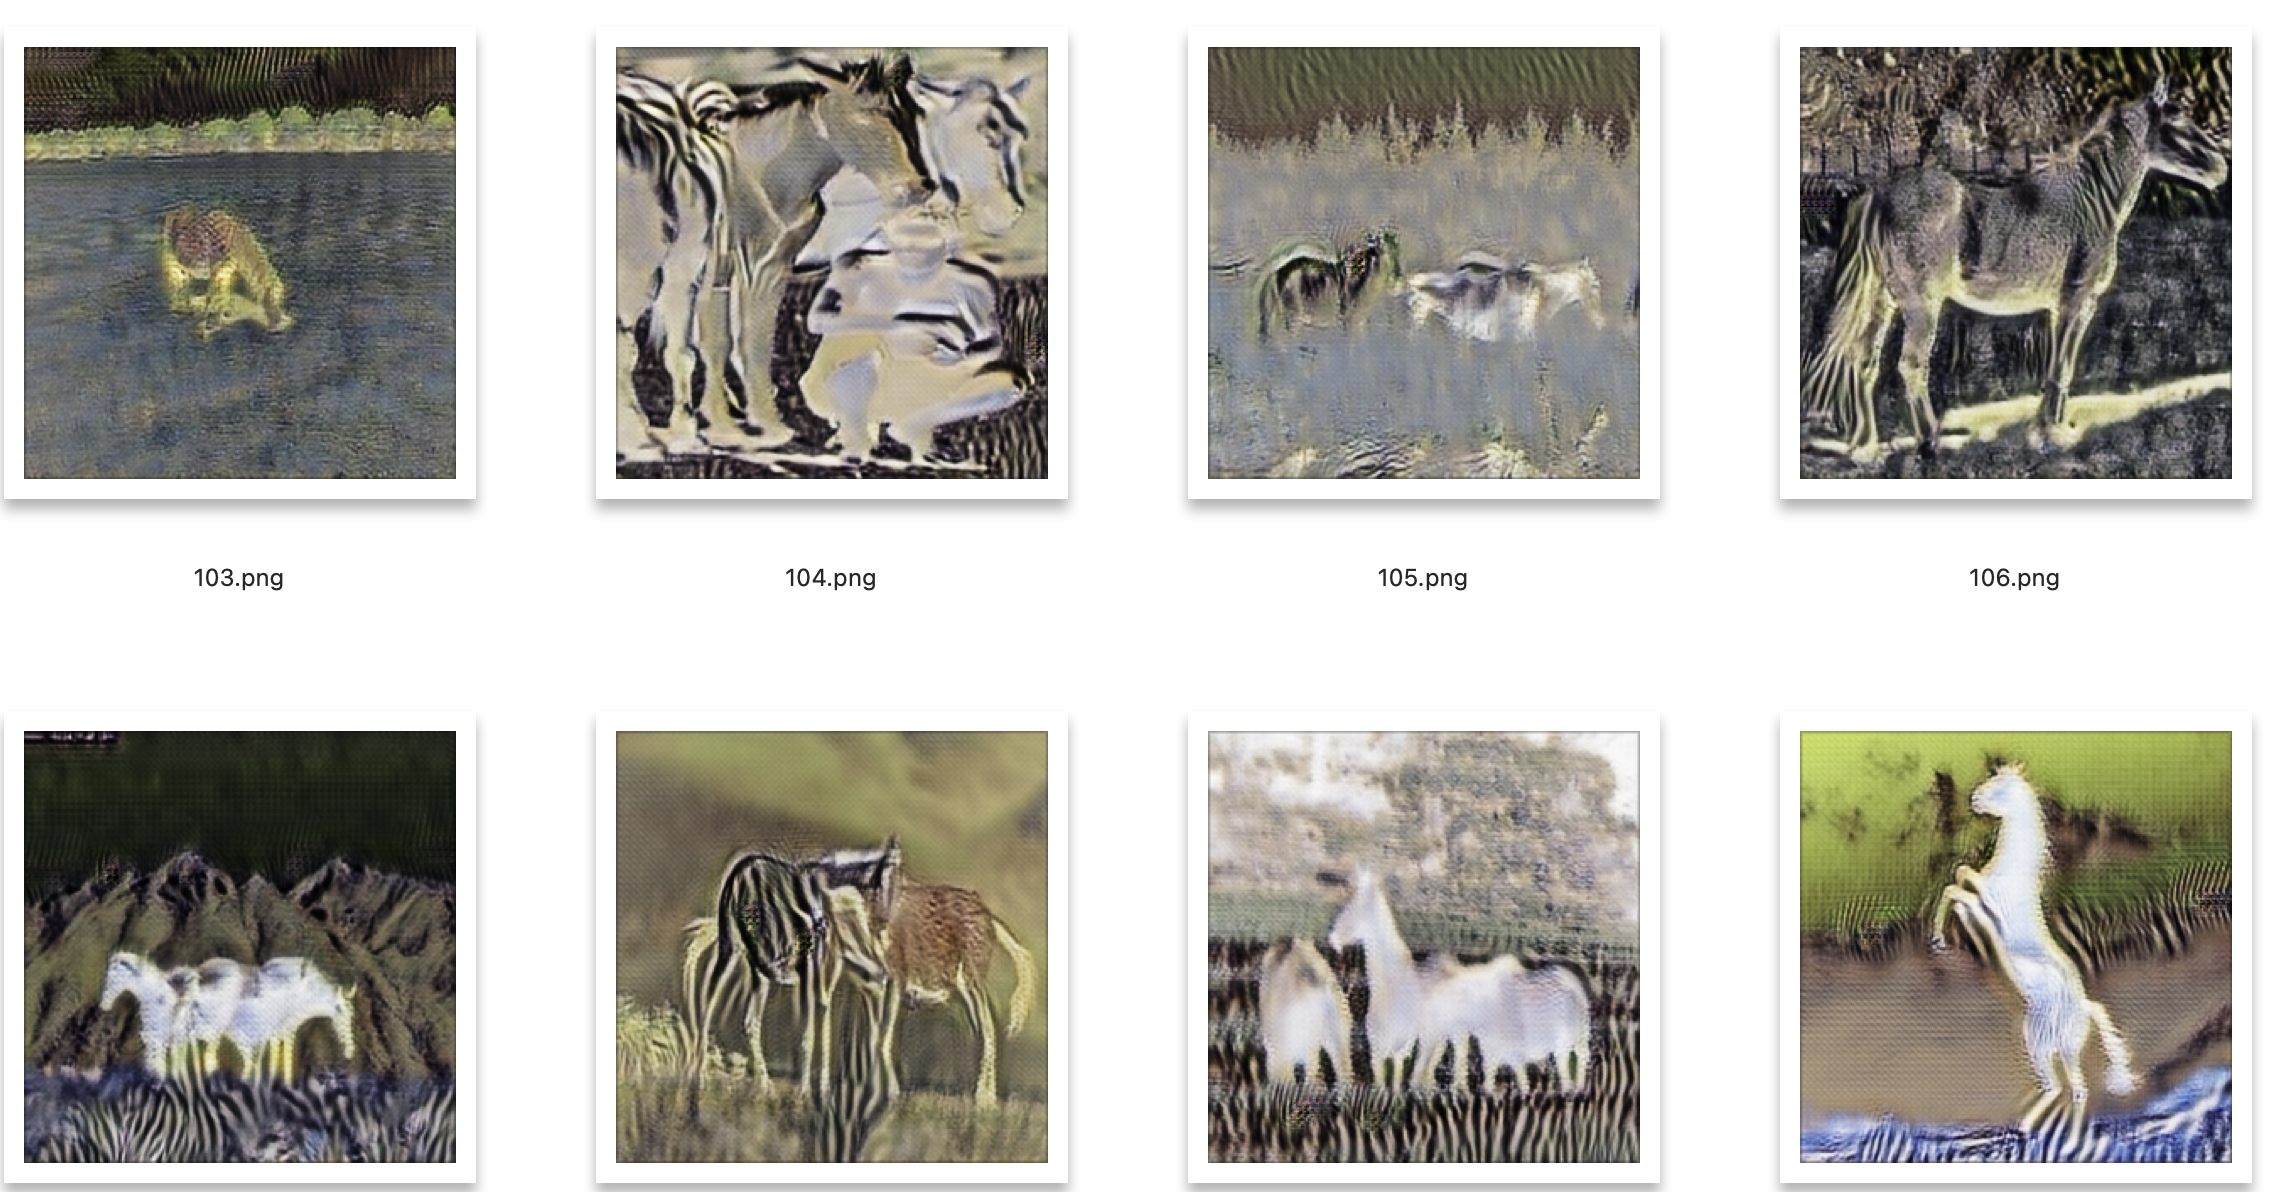
\includegraphics[width=1\textwidth]{Images/test_horse_zebra.png}
    \caption{Output Result for Image translation from \textbf{Horse to Zebra}}
    \label{fig:test_horse_zebra}
\end{figure}

\begin{figure}[htbp]
    \centering
    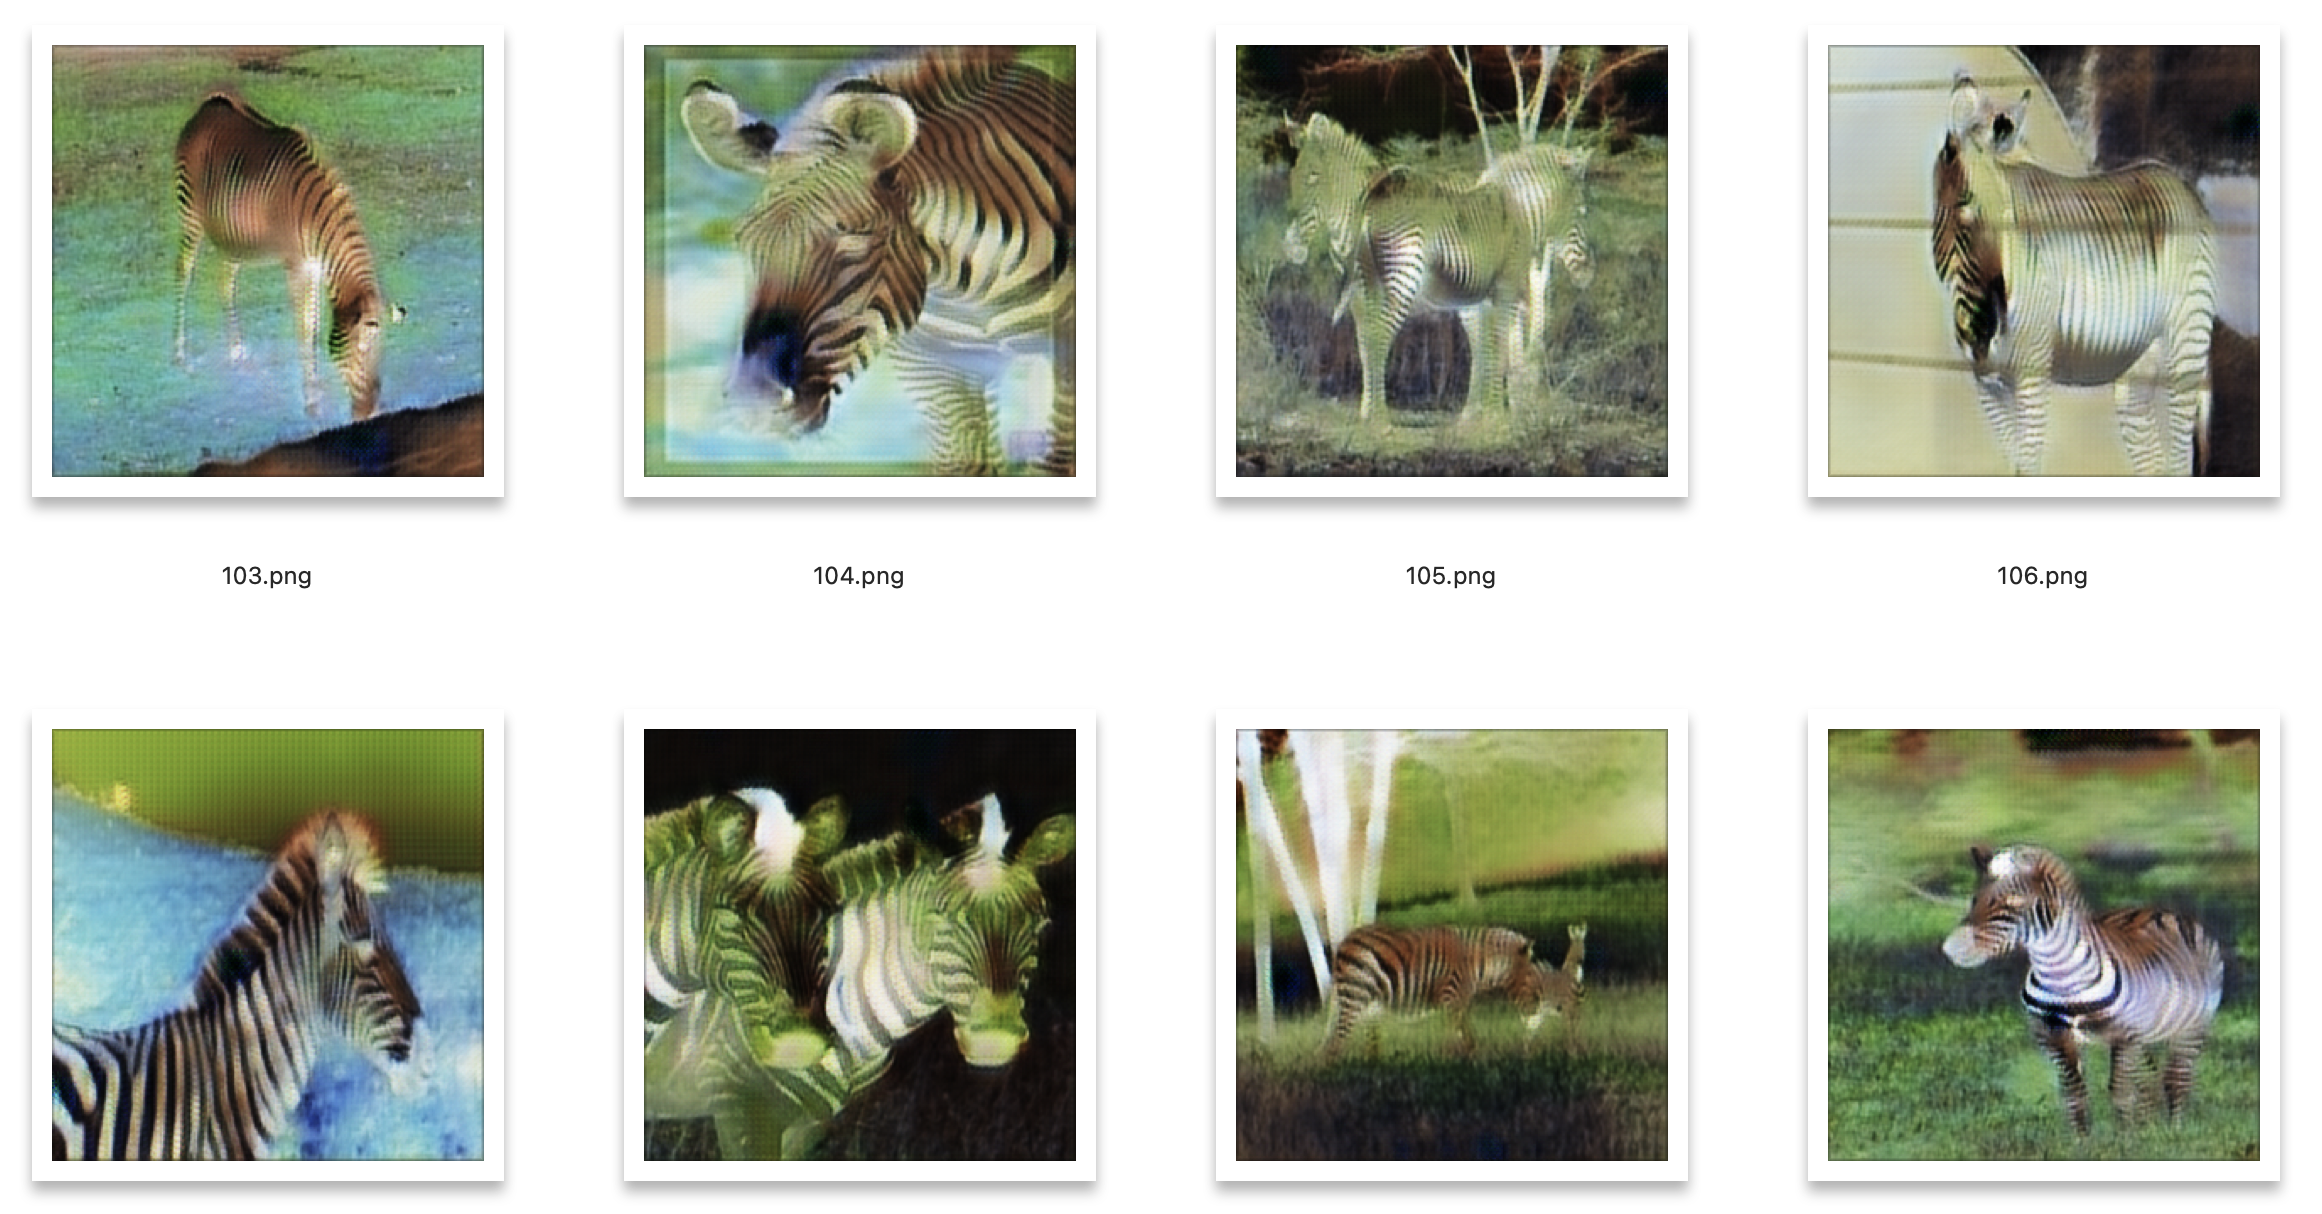
\includegraphics[width=1\textwidth]{Images/test_zebra_horse.png}
    \caption{Output Result for Image translation from \textbf{Zebra to Horse}}
    \label{fig:test_zebra_horse}
\end{figure}

\section{Generated Images on HyperKvasir Dataset:}


The CycleGAN model has been trained for 100 epochs on HyperKvasir Dataset, on 5255 images of "Original images" and "Syntehtic images" each. The trained model is saved for model checkpoint cycleGAN\_HK\_41800.pth. In this section, we evaluate the generative capabilities of the CycleGAN model trained on the HyperKvasir dataset. We begin by loading the pre-trained CycleGAN model from the specified checkpoint. The model consists of two generators: one for transforming images from domain A to domain B (gen\_AB) and another for transforming images from domain B to domain A (gen\_BA). We initialize these generator models and load their respective state dictionaries.

Transformations are defined for preprocessing the input images. These transformations include resizing the images to 256x256 pixels, converting them to tensors, and normalizing them. Images from the testA and testB folders, with 1000 images each, are then loaded into separate lists (testA\_images and testB\_images, respectively). These images represent the real images from domains A and B, respectively.

Directories are created to store the generated images. Subdirectories named "testA\_to\_B" and "testB\_to\_A" are created within a directory named "generated\_images". The model is then tested on the images from the testA and testB folders. For each image in testA, it undergoes an Image-to-Image translation process from domain A to domain B using generator G\_A. Similarly, for each image in testB, it undergoes a translation from domain B to domain A using generator G\_B.

During the testing process, each image is loaded, processed, and passed through the corresponding generator. The generated images are then saved in PNG format in the appropriate directories. Progress is logged as each image is processed. The sample of 10 output images translated from original image to synthetic images (domain A to domain B) is shown in \ref{fig:Output_A_B}, we can see that our model has tried to generate the blue circle area in the translated images. Similarly, the sample of 10 output images translated from synthetic image to original images (domain B to domain A) is shown in \ref{fig:Output_B_A}, we can see that our model has tried to remove the blue circle area in the translated images . 

\begin{figure}[htbp]
    \centering
    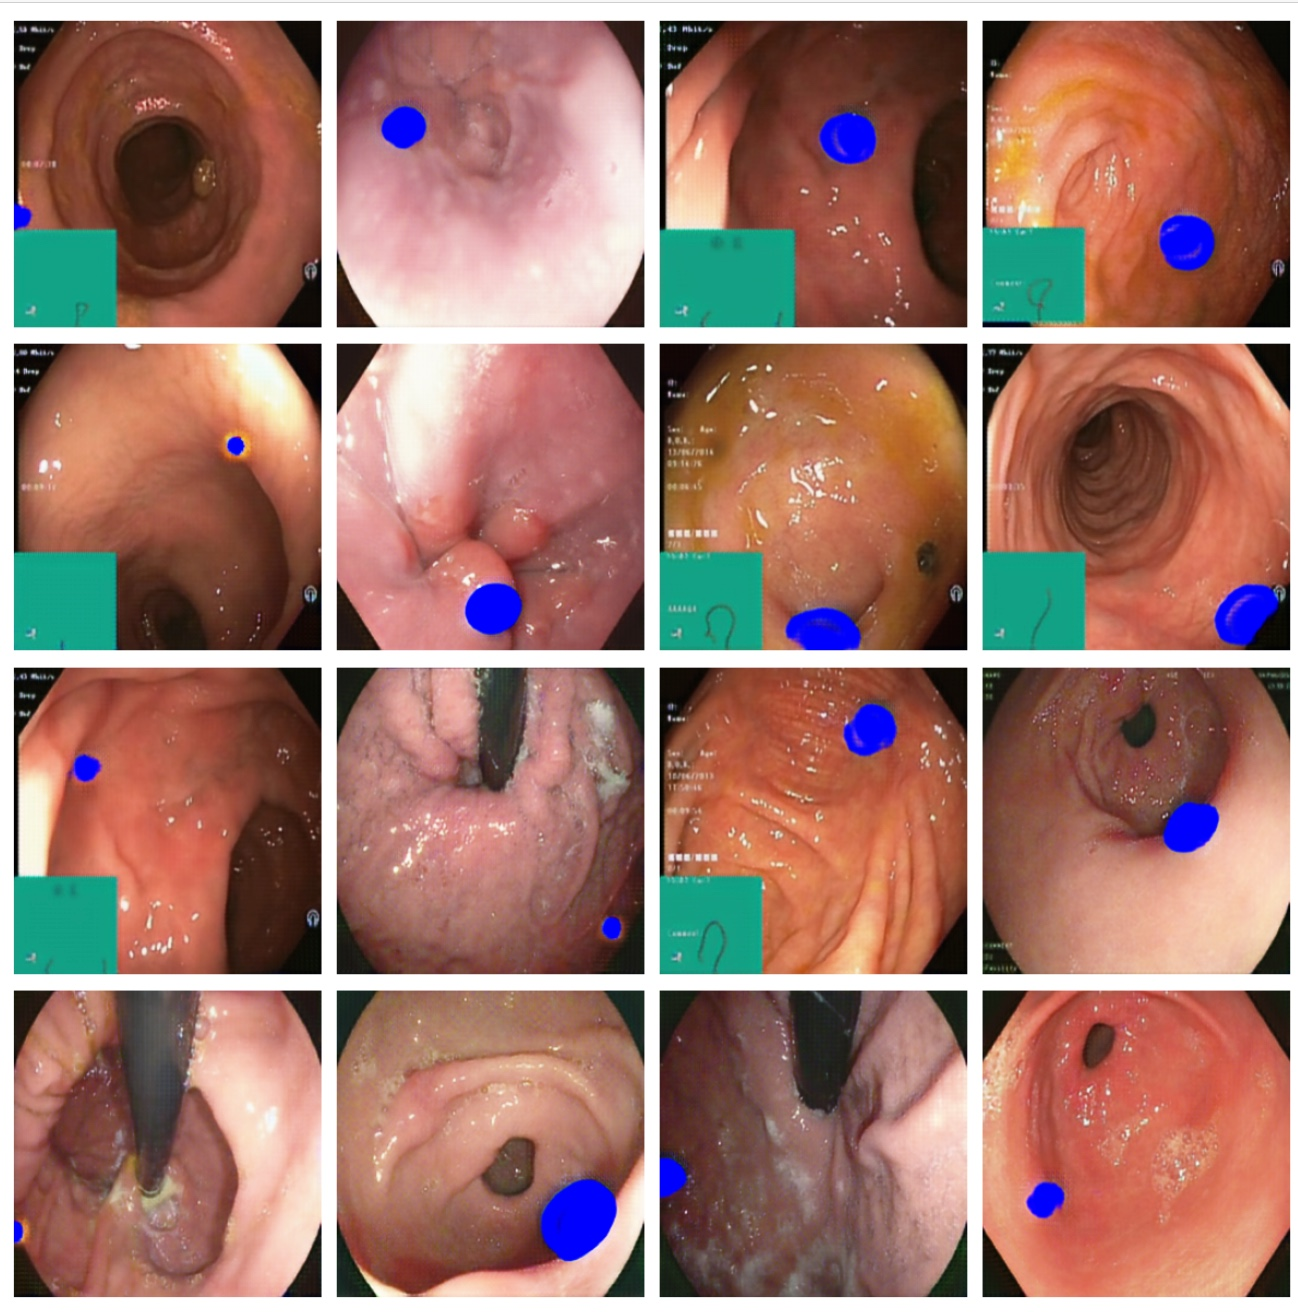
\includegraphics[width=1\textwidth]{Images/Output_A_B.jpeg}
    \caption{Image translation from \textbf{Healthy images to Synthetic Images}}
    \label{fig:Output_A_B}
\end{figure}

\begin{figure}[htbp]
    \centering
    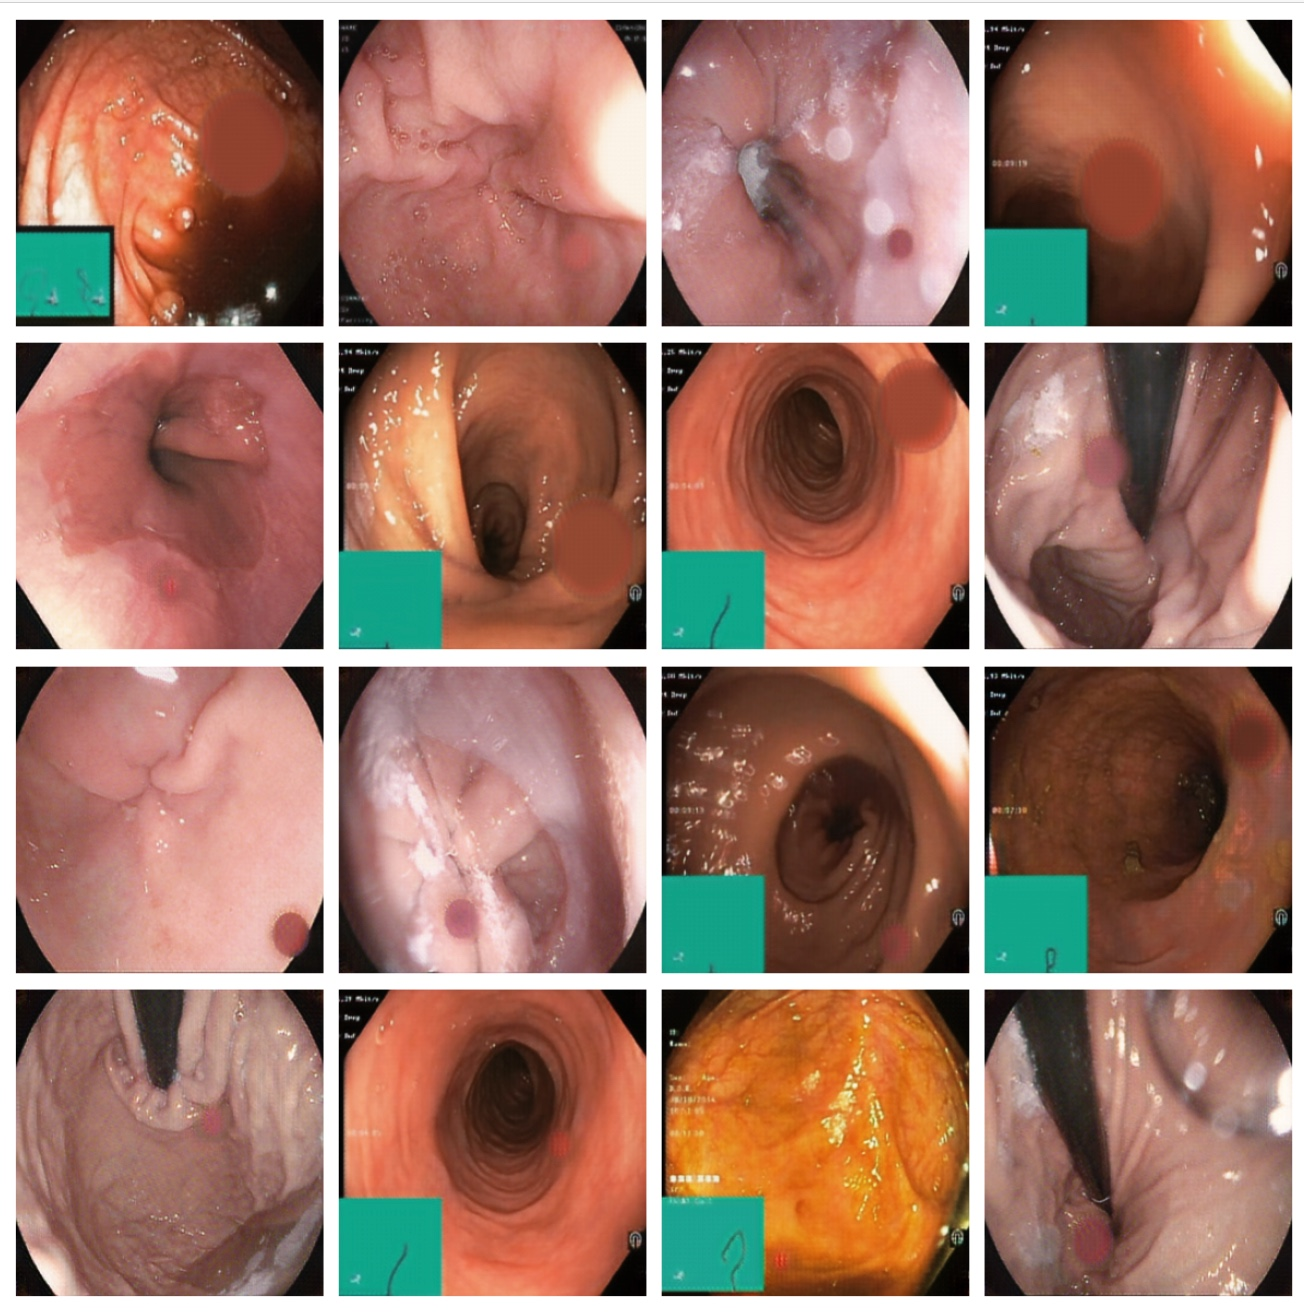
\includegraphics[width=1\textwidth]{Images/Output_B_A.jpeg}
    \caption{Image translation from \textbf{Synthetic images to Healthy Images}}
    \label{fig:Output_B_A}
\end{figure}

\section{Training Loss Analysis}

In the training phase of the CycleGAN model, monitoring the loss functions of both the generator and discriminator is crucial. This section provides an analysis of the training losses based on the data obtained from the training logs. The training logs, stored in a CSV file, are loaded into a pandas DataFrame. From the preprocessed training logs, the columns containing the generator and discriminator losses are extracted. Additionally, the columns representing the epochs and steps are also extracted. These values are essential for plotting the losses over the training duration.

The generator and discriminator losses are plotted against the training steps as shown in . The generator loss represents the discrepancy between the generated images and the target domain images, while the discriminator loss measures how well the discriminator distinguishes between real and fake images. The plotted graph provides a visual representation of how the losses evolve over the training process as shown in \ref{fig:Training_Loss}. The graph indicates that the generator loss is reducing with the steps.


\begin{figure}[htbp]
    \centering
    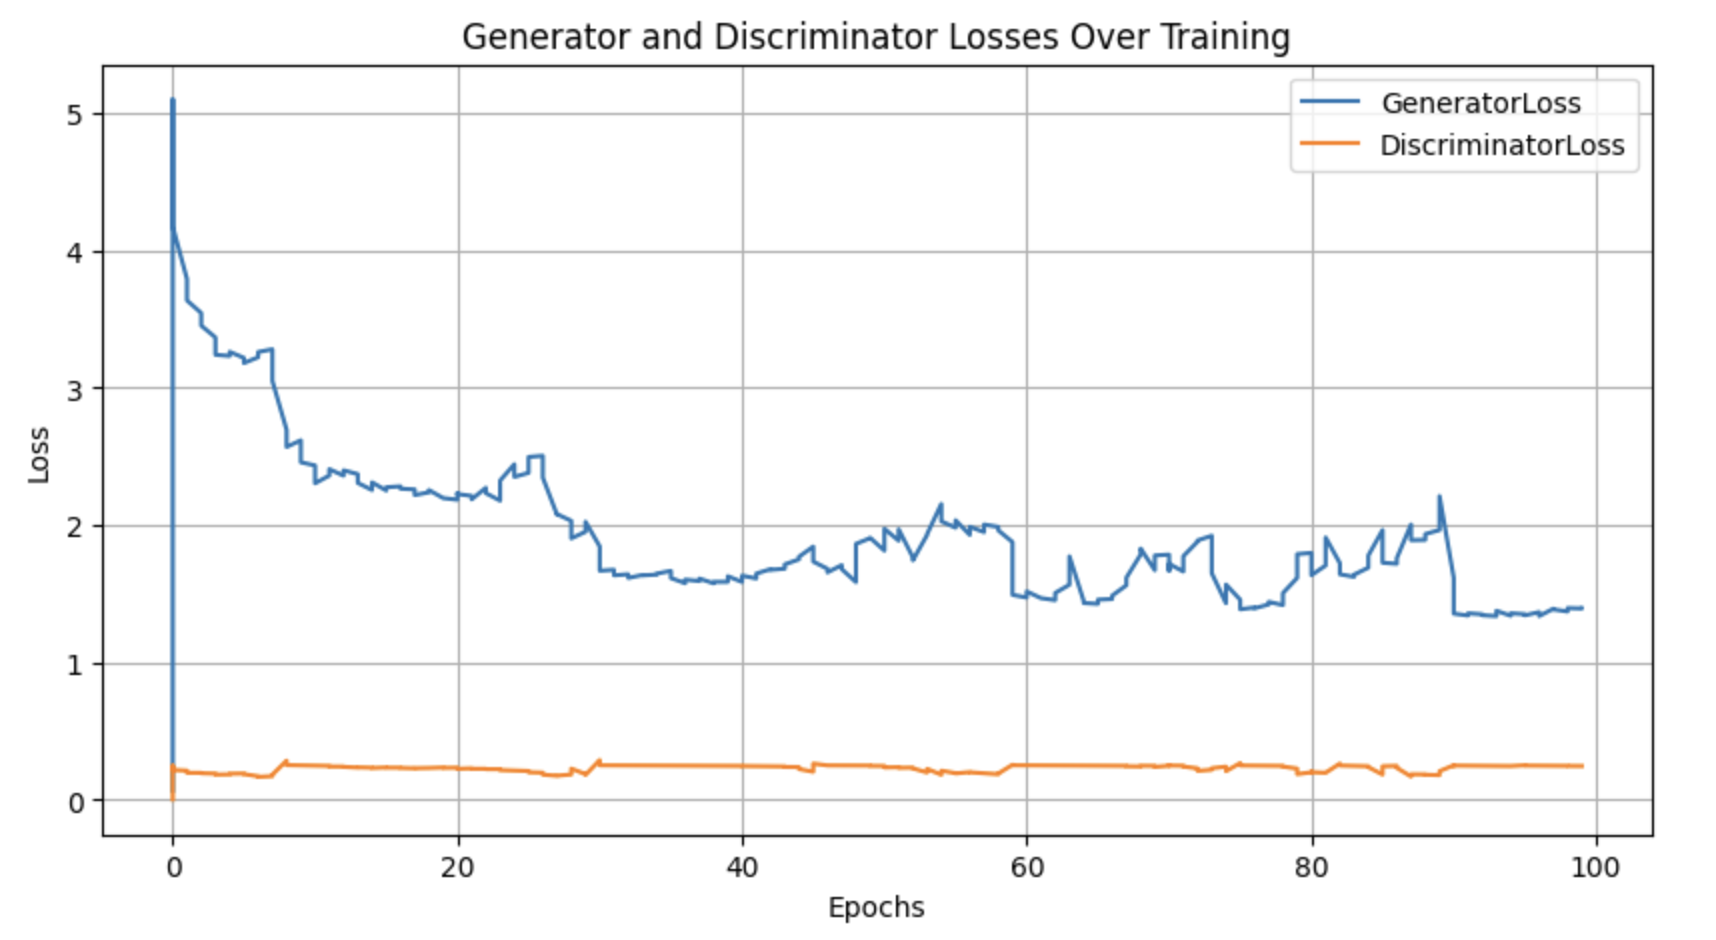
\includegraphics[width=1\textwidth]{Images/Training_Loss.png}
    \caption{Training Loss after 100 iterations}
    \label{fig:Training_Loss}
\end{figure}

\textbf{Observation}
There is an overall trend of reduction in generator loss over time. This downward trajectory indicates that the model gradually improves its ability to generate high-quality translated images that closely resemble the target domain. The reduction in loss reflects the model's increasing proficiency in capturing and replicating the desired features and characteristics of the target images.The discriminator loss starts very low in the initial epoch, showing the initial discriminator model could easily distinguish real from generated images. It then stabilizes, suggesting the generator and discriminator models have reached a more balanced state.
In the later stages, the discriminator loss decreases, indicating the discriminator model is becoming more effective at distinguishing real and generated images, likely due to the generator model's continued improvement. The observed fluctuations and trends in both generator and discriminator losses suggest that the CycleGAN model converges towards an optimal solution over time.
\section{Evaluation Metrics}

The evaluation of the CycleGAN model involves assessing the quality of the generated images compared to the true images. 
The trained CycleGAN model is loaded and set to evaluation mode using the eval() method. This ensures that the model is not affected by gradients during evaluation. The dataset is prepared using an appropriate dataloader to facilitate the evaluation process.

SSIM measures the similarity between the original and generated  images, taking into account luminance, contrast, and structure. PSNR measures the quality of the reconstruction by computing the ratio between the maximum possible power of a signal and the power of corrupting noise that affects the fidelity of its representation. FID assesses the similarity between two distributions of images by comparing their feature representations extracted from an Inception V3 model pretrained on ImageNet. It calculates the distance between the mean and covariance of the feature representations of the real and generated images.

For our thesis, real images and generated images are loaded and resized to a common size (256x256) for consistency in evaluation. Real images are obtained from the test datasets, while generated images are outputs from the trained CycleGAN model. SSIM and PSNR are calculated for both translation directions (A to B and B to A) by comparing corresponding pairs of real and generated images. The mean SSIM and PSNR values are computed as evaluation metrics. FID is calculated using a function that extracts feature representations from an Inception V3 model for both real and generated images. The feature statistics (mean and covariance) are then compared to compute the FID score for each translation direction. The evaluation metrics obtained for our objective is shown in \ref{fig:Evaluation Metrics}.

The high SSIM values and PSNR values for both translation directions indicate that the generated images closely resemble the ground truth images, with minimal distortion and high fidelity. The low FID scores further reinforce the notion of realistic image generation, with the distributions of the generated images closely matching those of the real images in both domains.

\begin{figure}[htbp]
    \centering
    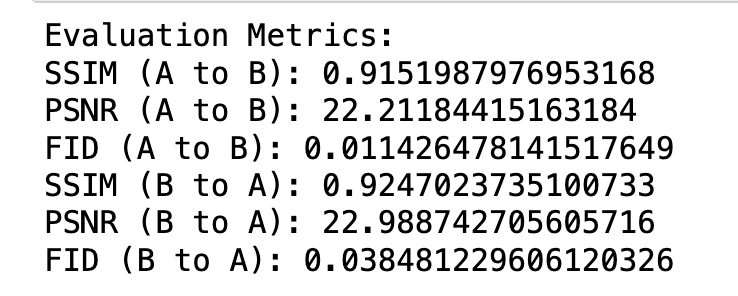
\includegraphics[width=1\textwidth]{Images/Evaluation Metrics.png}
    \caption{Evaluation Metrics}
    \label{fig:Evaluation Metrics}
\end{figure}

\textbf{SSIM (Structural Similarity Index)}

The SSIM (A to B) value of 0.915 indicates a high degree of structural similarity between the generated images in domain B and the corresponding true images in domain B. This suggests that the generated images closely resemble the target domain images in terms of structural features, including texture, contrast, and overall appearance. Similarly, the SSIM value of 0.925 for the B to A translation indicates a high degree of similarity between the generated images in domain A and the corresponding ground truth images in domain A. The generated images closely match the characteristics of the target domain images, demonstrating effective image translation from domain B to domain A.

\textbf{PSNR (Peak Signal-to-Noise Ratio)}
The PSNR value of 22.21 dB, for A to B Translation, quantifies the quality of the reconstructed images in domain B compared to the ground truth images in domain B. A higher PSNR value indicates lower noise and better fidelity of the generated images to the original images. Similarly, the PSNR value of 22.99 dB for the B to A translation measures the quality of the reconstructed images in domain A compared to the ground truth images in domain A. The higher PSNR value suggests minimal distortion and high fidelity in the generated images.

\textbf{FID (Fréchet Inception Distance)}
A to B Translation (FID = 0.011):
The FID score of 0.011 for A to B Translation, represents the distance between the feature distributions of the generated images in domain B and the real images in domain B. A lower FID score indicates a closer match between the distributions, signifying high similarity and realism in the generated images. Conversely, the FID score of 0.038 for the B to A translation measures the distance between the feature distributions of the generated images in domain A and the real images in domain A. Despite being slightly higher than the A to B translation, the FID score still indicates a relatively close match between the distributions, suggesting realistic image generation.

\textbf{Variability Score Analysis}

The variability score quantifies the level of variability or divergence between the original images and their corresponding translated images generated by the CycleGAN model. This section presents an analysis of the variability scores obtained from the comparison of synthetic data (original images) and translated data (images translated from domain A to domain B). This score is calculated for 1000 images for each set. For each pair of original and translated images, the variability score is computed as the mean absolute difference between corresponding pixel values. This score quantifies the extent of variation between the images. The variability scores are normalized to ensure consistency and comparability across different datasets. Normalization scales the scores to a range from 0 to 1, facilitating easier interpretation and analysis.

The mean variability score is calculated as the average of the normalized variability scores. For our experiment we got Mean Variability Score (Normalized): 0.502. The variability score indicates that the model effectively preserves essential features and characteristics during the image translation, ensuring that the translated images remain visually similar to their original counterparts.

\section{Reconstruction of Images}

The reconstruction of images using the trained CycleGAN model involves translating an image from one domain to another and then reversing the translation to reconstruct the original image. This section elaborates on the process of image translation and reconstruction and presents the results obtained from the trained model.

The trained CycleGAN model is loaded from our  cycleGAN\_HK\_41800.pth checkpoint file. Two generator models (gen\_AB and gen\_BA) are created, corresponding to the translation from domain A to B and from domain B to A, respectively. The weights from the checkpoint are loaded into the generator models. Transformations are defined to preprocess input images before feeding them into the model for translation and reconstruction. These transformations include resizing the images to the target shape and converting them into tensors.

A function named translate\_and\_reconstruct is defined to perform the translation and reconstruction process for a given input image. This function takes the path of an input image as input, loads the image, performs translation from Healthy to Synthetic to Healthy Images using the generator models, and finally plots the original image, translated image, and reconstructed image side by side as shown in \ref{fig:A-B-A} . Similarly ,it performs translation from Synthetic to Healthy to Synthetic Images using the generator models, and finally plots the original image, translated image, and reconstructed image side by side as shown in \ref{fig:B-A-B}. A sample of 10 images are generated for both the domains. 

\begin{figure}[htbp]
    \centering
    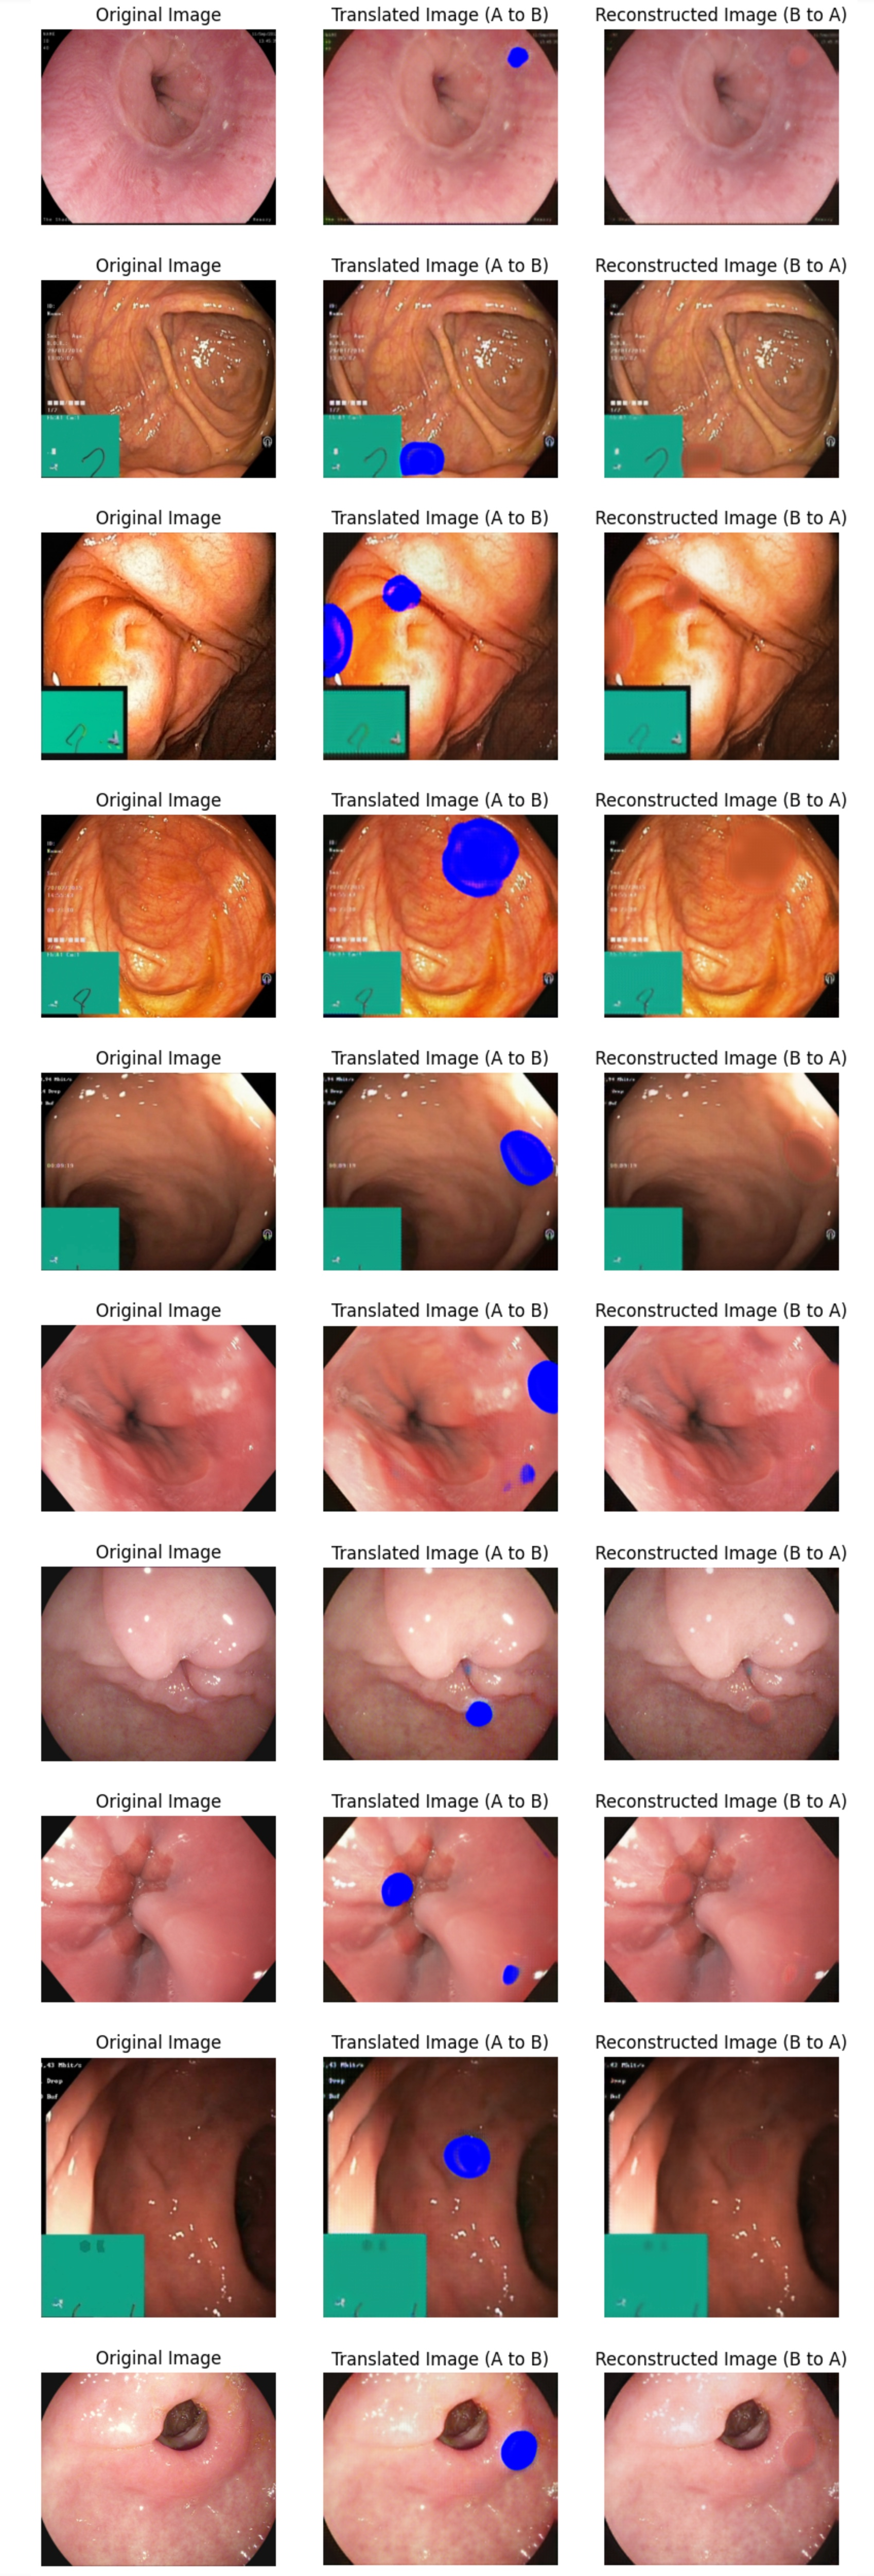
\includegraphics[width=0.5\textwidth]{Images/A-B-A.jpeg}
    \caption{Reconstruction of images from \textbf{Healthy to Synthetic to Healthy Images}}
    \label{fig:A-B-A}
\end{figure}

\begin{figure}[htbp]
    \centering
    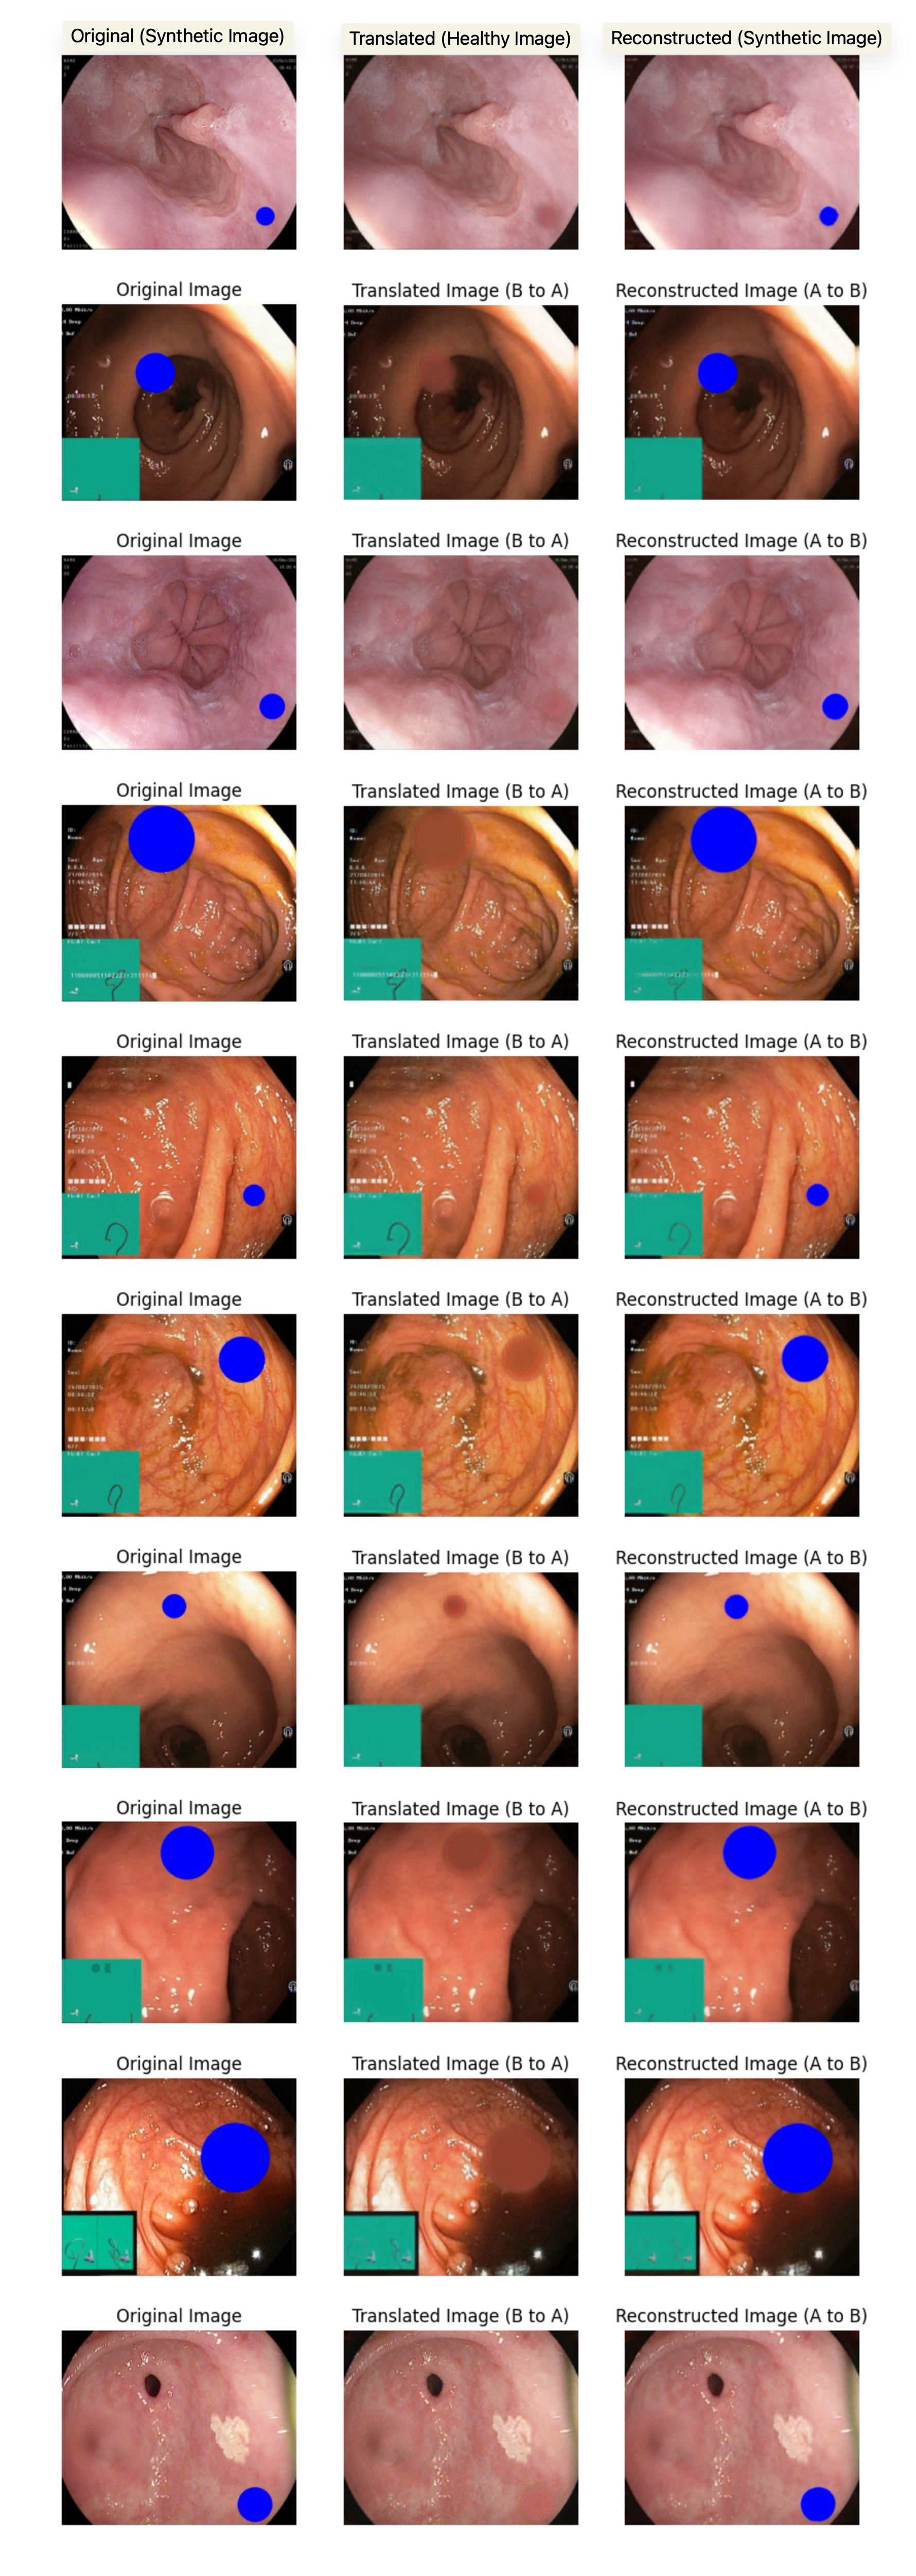
\includegraphics[width=0.5\textwidth]{Images/B-A-B.jpeg}
    \caption{Reconstruction of images from \textbf{Synthetic to Healthy to Synthetic Images}}
    \label{fig:B-A-B}
\end{figure}

\section{Analyses of distribution of Blue circle Coordinates}

The distribution analysis focuses on examining the distribution of the blue circle area in synthetic images (original images) and translated images (images translated from domain A to domain B) generated by the CycleGAN model. This section elaborates on the process of extracting coordinates from the images, analyzing their distributions, and interpreting the findings. The images from both directories are resized to a common target size of 256x256 pixels using the resize\_image function. This ensures uniformity in image dimensions for accurate analysis.

\textbf{Coordinate Extraction: }The original images are converted from the RGB color space to the HSV (Hue, Saturation, Value) color space. HSV is often preferred for color-based image processing tasks due to its ability to separate intensity information (value) from color information (hue and saturation). A range of blue color values in the HSV color space is defined to isolate blue regions within the images. This range is specified using lower and upper threshold values for the hue, saturation, and value channels. By defining this range, the algorithm can identify pixels that fall within the specified blue color range.

The HSV representation of the image is thresholded using the defined range of blue color values. This process involves setting pixels to white (255) if their HSV values fall within the specified blue range, and to black (0) otherwise. As a result, a binary image mask is created, where white pixels represent the blue regions of interest and black pixels represent non-blue regions. Contours are the outlines of objects or shapes within an image. In this step, the contours of the blue regions in the binary mask are identified using contour detection algorithms. These contours represent the boundaries of the blue areas in the image. For each contour detected, the centroid (center of mass) of the contour is computed using the moments of the contour. The moments provide statistical information about the shape and spatial distribution of the contour. By calculating the centroid, the algorithm can determine the center coordinates (x, y) of the blue circle area.

\begin{figure}[htbp]
    \centering
    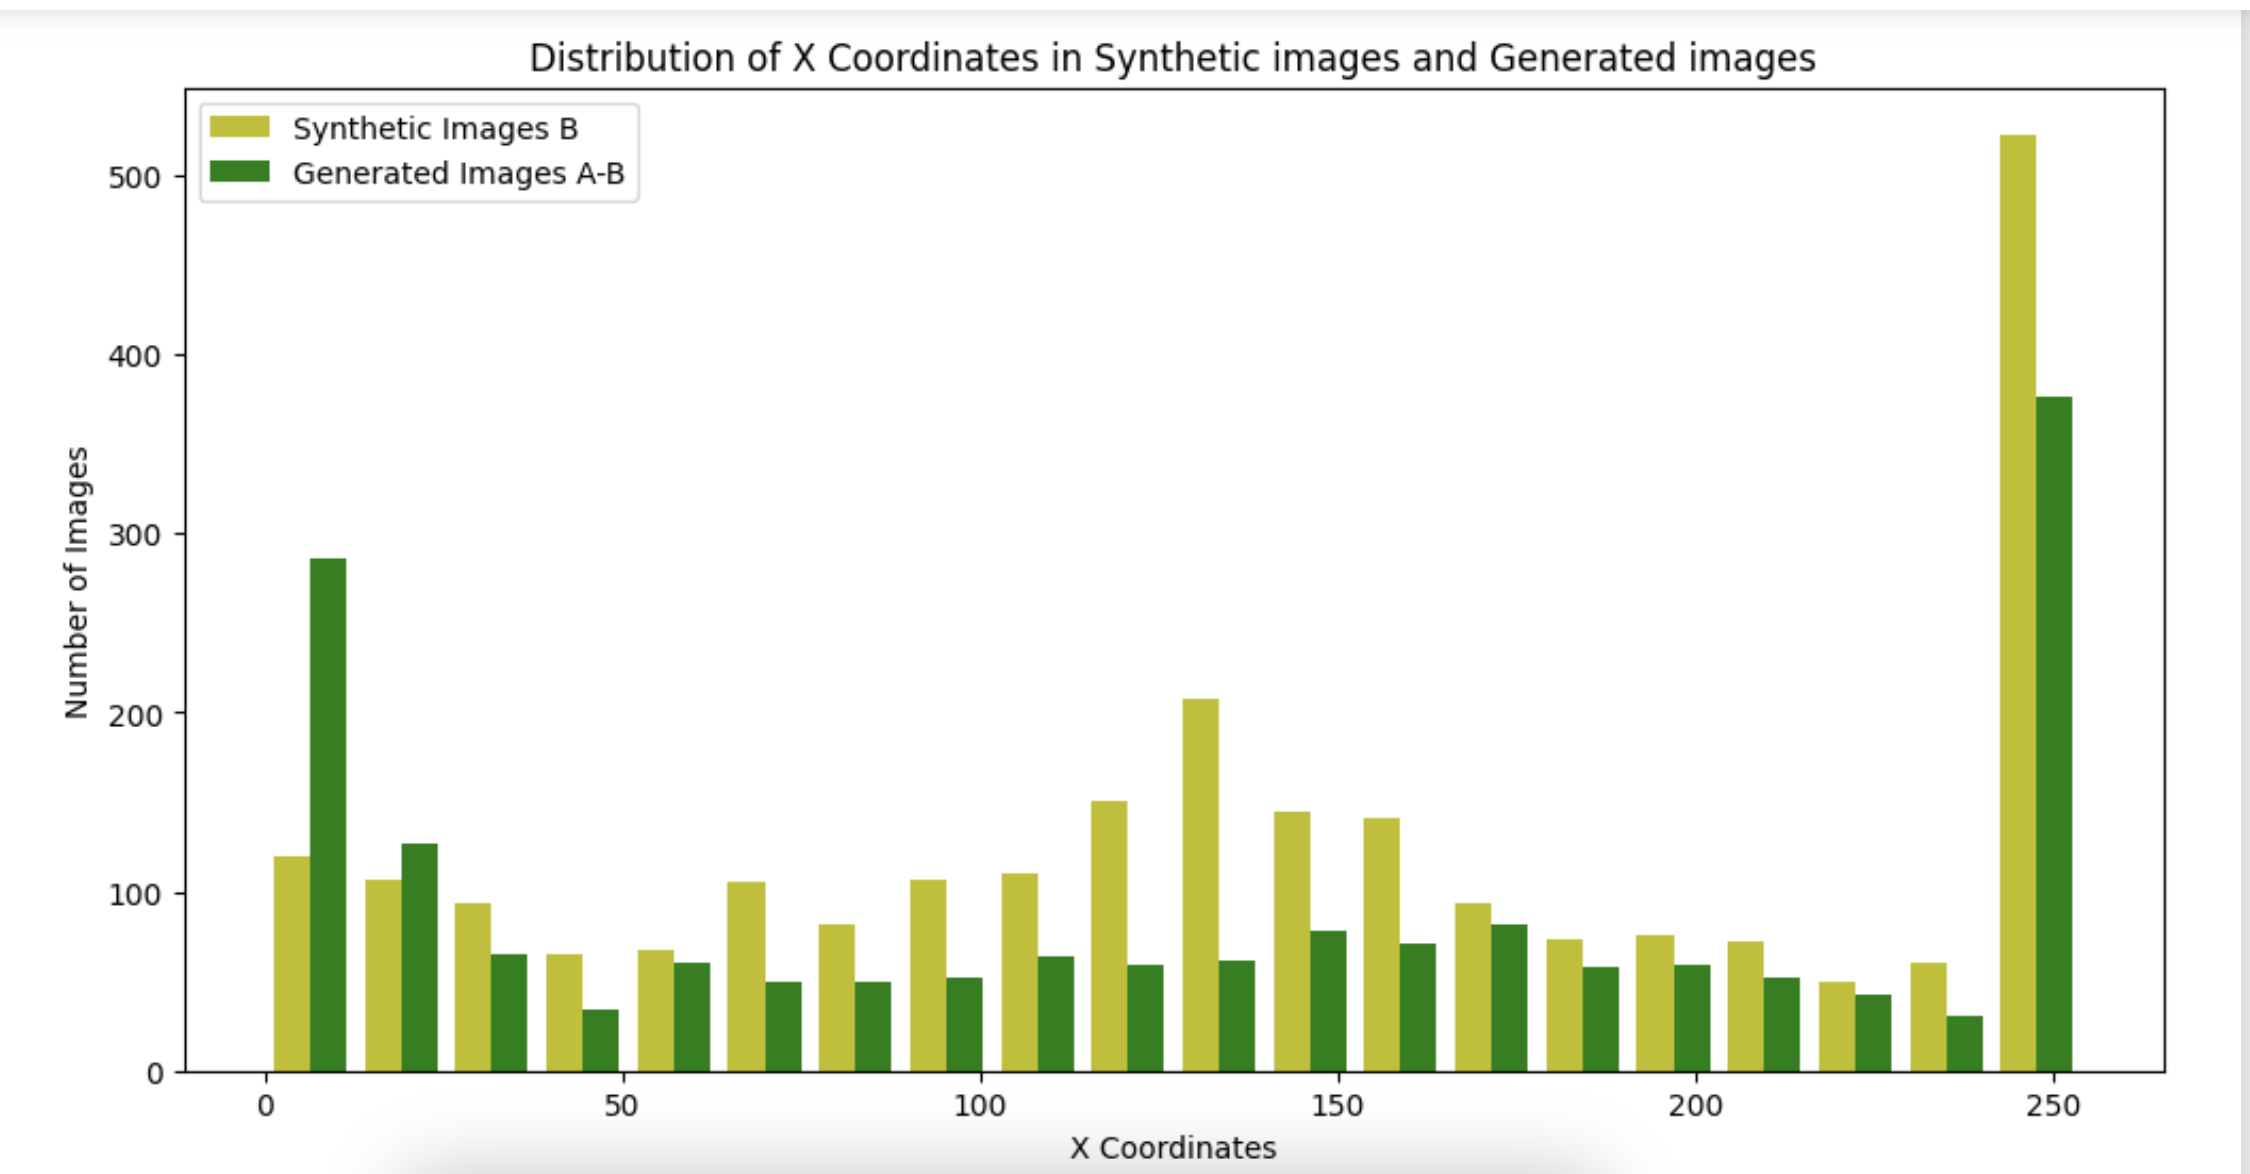
\includegraphics[width=1\textwidth]{Images/x_coordinates.png}
    \caption{Histogram to analyse the distribution of X-coordinates of Blue circle over Healthy and Synthetic images}
    \label{fig:x_coordinates}
\end{figure}

\begin{figure}[htbp]
    \centering
    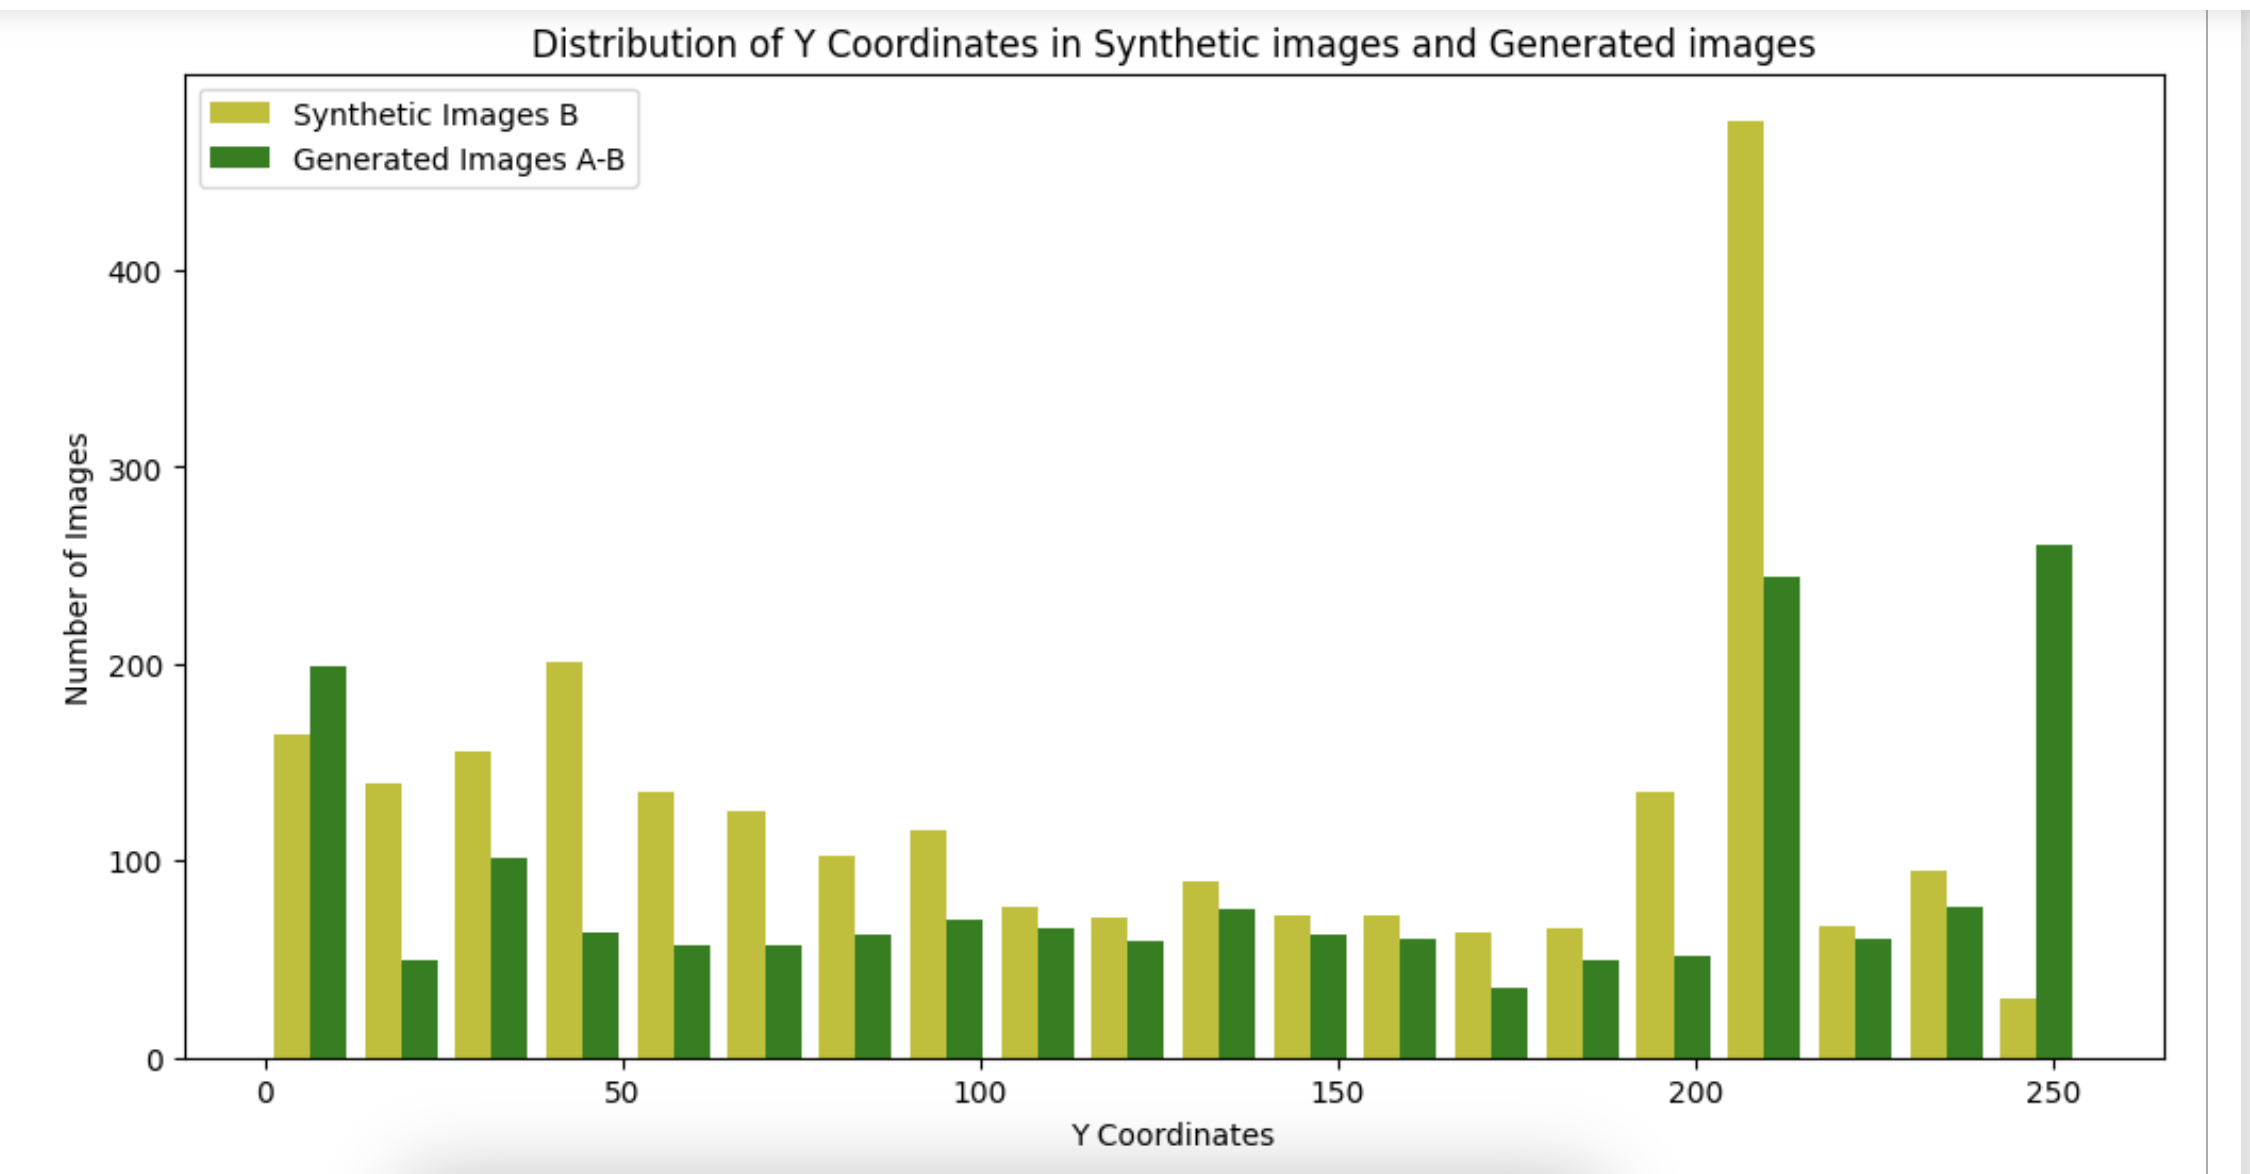
\includegraphics[width=1\textwidth]{Images/y_coordinates.png}
    \caption{Histogram to analyse the distribution of Y-coordinates of Blue circle over Healthy and Synthetic images}
    \label{fig:y_coordinates}
\end{figure}

\textbf{Observations:}
The X and Y coordinates of the blue circle centers are extracted from both sets of images (synthetic images and translated images).
Two histograms are plotted to visualize the distribution of X and Y coordinates separately for both sets of images as shown in \ref{fig:x_coordinates} and \ref{fig:y_coordinates}. Each histogram represents the frequency of occurrence of coordinates along the respective axis.
Despite differences in the exact frequency distribution, there are intervals along the X and Y coordinates where synthetic and generated images exhibit similar frequency. This indicates that certain patterns of blue patch distribution are shared between the two datasets, which shows the  similarities in the spatial organization of polyp-like structures. In some intervals, both synthetic and generated images shows similar trends in frequency distribution along the X and Y coordinates. This consistency in patterns suggests that the CycleGAN model may learn common spatial characteristics of polyps and produce them in the generated images.


\section{Analyses of distribution of size of Blue Circle Area}
In this section, we will do the analysis of the distribution of blue circle areas within the synthetic images and generated images produced by the CycleGAN model. 

\textbf{Blue circle Area Detection :}
To detect the presence of blue patches within the images, we employed a color-based detection approach using OpenCV. The images were first converted to the HSV color space to better isolate the blue color range. A predefined range of HSV values corresponding to blue hues was utilized to create a mask highlighting the blue regions within the images. Contour detection was then employed to identify individual blue patches within the images. We analyzed two sets of images: synthetic images augmented with blue round shapes at random locations within the original healthy image dataset, and generated images resulting from the translation of healthy images to cancer images with polyps by the CycleGAN model (referred to as 'Generated Images A-B'). A total of 1000 images were randomly sampled from each set for analysis.

The histogram presented in \ref{fig:Blue_circle_area} illustrates the distribution of blue patch areas within the synthetic images and generated images. Each bin in the histogram represents a range of blue patch areas in pixels, while the height of the bars indicates the frequency of images containing blue patches falling within each respective range.

\begin{figure}[htbp]
    \centering
    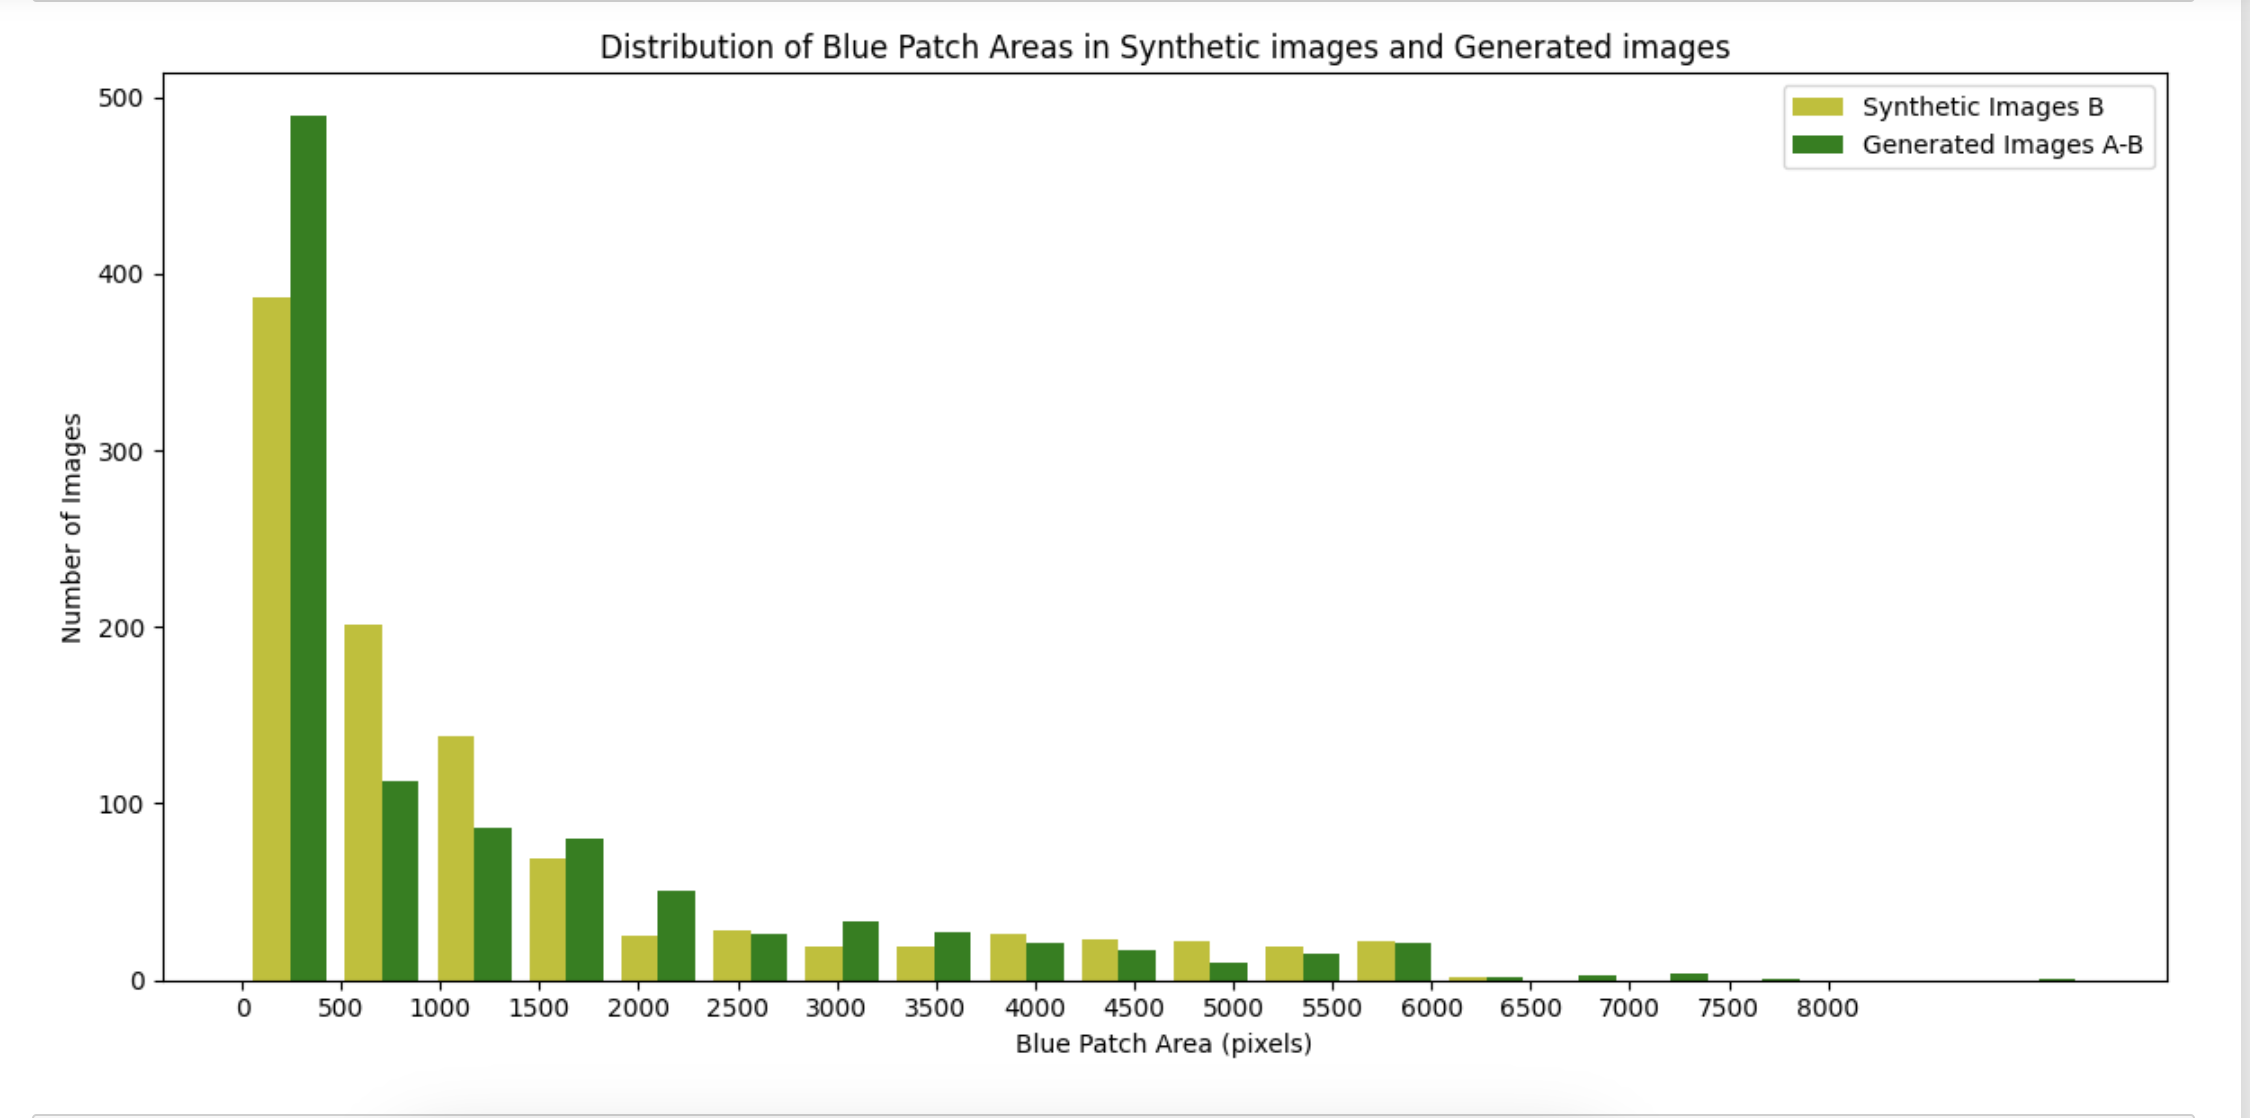
\includegraphics[width=1\textwidth]{Images/Blue_circle_area.png}
    \caption{Histogram to analyse the the distribution of area covered in pixels by Blue circle over Healthy and Synthetic images}
    \label{fig:Blue_circle_area}
\end{figure}

\textbf{Observations:}

The histogram reveals similar patterns in the distribution of blue patch areas between the synthetic images and generated images.
In the synthetic images, the majority of blue circle area fall within the range of 0 to 500 pixels, with a frequency of around 400 images. This suggests that smaller blue patches are more prevalent in the synthetic dataset. Similarly, the distribution of blue patch areas is maximum in the same pixel range, with around 500 images.
As the blue patch areas increase, the frequency gradually decreases in both datasets, indicating a decreasing frequency of larger blue patches. Both the synthetic images and the generated images have a small number of outliers with very large blue patch areas (6000-8000 pixels). These outliers may represent images with unusual or blue patch distributions.

\chapter{Discussion}

Image-to-Image (I2I) translation methods have gained significant attention in recent years for their ability to transform images from one domain to another while preserving essential characteristics \cite{I2I} . These methods have numerous applications across various domains, including medical imaging, where the translation of images between different modalities or domains can aid in diagnosis, treatment planning, and medical research. In this study, we focused on analyzing the generative properties of I2I translation methods, specifically utilizing the CycleGAN model \cite{CycleGAN} , within the context of medical image analysis. Our primary objective was to investigate the extent to which these methods can generate translations with diverse realistic properties, with a particular emphasis on the Hyper Kvasir dataset and its application to polyp detection in gastrointestinal endoscopy images.

\section{Image to Image Translations}
We employed the CycleGAN model due to its effectiveness in learning mappings between two image domains without the need for paired data. 
Our analysis focused on evaluating the reality and diversity of the generated translations, particularly focusing on blue circle area imitating polyps' variations in position, size, and shape. The Hyper Kvasir dataset, consisting of gastrointestinal endoscopy images has been used for training and evaluation \cite{HyperKvasir_Dataset} . Through extensive experimentation and training, we observed that the CycleGAN model was capable of generating diverse translations that closely resembled original images from the target domain. 

\section{Strengths and Limitations of CycleGAN}
Despite the overall effectiveness of the CycleGAN model, several challenges and limitations were faced during the analysis. One significant challenge was the requirement for large training data to capture the diversity of image translations accurately. While the Hyper Kvasir dataset offered a large collection of images and video, We had to limit our training data due to the limited time frame of the master thesis and limited availability of GPU resource, . 

\section{Future Work} 
To address the challenges and further enhance the generative capabilities of Image-to-Image translation methods, several future research directions can be explored. Firstly, using the whole HyperKvasir datasets which will provide more extensive range of variations in gastrointestinal endoscopy images , which could help improve the model's ability to capture rare or unusual cases. Furthermore, exploring alternative architectures, such as attention mechanisms, diffusion models or style transfer, may offer opportunities to enhance the diversity and reality of generated translations. Additionally, doing clinical evaluations to assess the practical utility of the generated images in real-world medical scenarios could provide valuable insights for future development and deployment.

Another suggestion to future work is to investigate if GANs can be used as a data augmentation method. A possible way to answer the question would be to test it on a classification network for semantic segmentation. GANs would be used to generate synthetic training data for the classification network. Several test could then be done with different amount of synthetic data. The performance of the classification network trained with different amount of synthetic data could then be evaluated. Which would indicate if GANs can be used as a data augmentation method.

\section{Answers to the Research Questions} 
\begin{enumerate}
\item Identification of Powerful and Reliable I2I Method
    
Through various literatre review , it was determined that the CycleGAN model is a powerful and reliable method for Image-to-Image translation (I2I) applications within the context of gastrointestinal endoscopy image enhancement and analysis. The model produced accurate translations between healthy image to cancer images with polyps.

\item Analysis of Generative Properties with Generative Model

The generative properties of our CycleGAN model was analysed with two different approach. Firstly, studying the distribution of locations and determining the coordinates of blue circles imitating polyps in cancer images in the generated images and synthetic images. Secondly, studying the distribution of area of blue circles in the generated images and synthetic images. 

\item Generation of Synthetic Image Data

The task of generating synthetic image data by introducing blue round shapes at random locations with random size within the original dataset of healthy images from the HyperKvasir dataset was successfull. The synthetic images was helpul in bringing variations in dataset for training I2I models which improved model performance.

\item Creation of Visual and Qualitative Evaluation Metrics

Visual output images were produced while testing and evaluating the model performance. Bar chart and histogram analyses were also carried out. Evaluation metrics sucha s SSIM, PSNR, FID were also calculated to carry out quantitative analysis.

\end{enumerate}

\chapter{Conclusion}

In this thesis, our aim was to explore the capabilities of Image-to-Image (I2I) translation methods, specifically focusing on their application within the area of medical imaging using the Hyper Kvasir dataset. Our goal aimed to address the challenges associated with generating diverse and realistic medical images, especially when there isn't much data available and privacy concers make it hard to collect data in the usual ways. In our study, we used the advantage of deep learning techniques, particularly the CycleGAN method, to develop a practical solution for synthesizing medical images directly from the Hyper Kvasir dataset. We worked on different parts of the project, from data preparation and model implementation to performance evaluation and distribution analysis.

Firstly, we carefully prepared the Hyper Kvasir dataset, making sure it could work with the CycleGAN framework. We also added some synthetic data to simulate different medical problems like polyps. This step was really important for setting up our later tests. After that, we worked on the development and implementation of a CycleGAN-based Image-to-Image translation specifically designed for medical image domain. We evaluated our trained cycleGANs models performance on qualitative metrics through visual inspections of the generated images and quantitative metrics such as calculating FID, SSIM and PSNR score. These evaluations helped us see how realistic and accurate the medical images were, especially in terms of the size, shape, and position of the simulated health issues.

Furthermore, our distribution analysis shed light on the patterns observed within the generated images, comparing them with real-world medical imagery to ascertain the fidelity of the translations. By measuring the variability in size and placement of simulated medical conditions, we gained valuable insights into the model's ability to produce diverse and accurate outputs. Additionally, we compared the images we generated with real medical images to see if they looked similar. By measuring the size and placement of the simulated medical problems, we learned more about how good our model was at making different and accurate images.

After evaluating our CycleGAN model on a different set of test data, we tested compared its performance with other I2I translation approaches. This comparison helped us understand the strengths and limitations of our approach, which will help others make better medical images in the future. Lastly, we carefully documented and reported our methodologies, experimental setup, and results. We discussed about our results and suggested ideas for future research to make medical images even better using methods like I2I translation. In summary, our study shows how I2I translation methods can make realistic and varied medical images, which could help healthcare providers diagnose illnesses better. By addressing the challenges of data scarcity and privacy concerns, our method can enhance computer-aided diagnosis systems and improve patient care in clinical settings.

\backmatter
\printbibliography
\end{document}